%%*************************************************************************
%%
%% Učení novou neznamou technologie.
%% V0.0
%% 2012/11/28
%% Timothy Hobbs
%% timothyhobbs@seznam.cz
%%
%%*************************************************************************
%%
%% Legal Notice:
%%
%% This code is offered as-is without any warranty either expressed or
%% implied; without even the implied warranty of MERCHANTABILITY or
%% FITNESS FOR A PARTICULAR PURPOSE! 
%% User assumes all risk.
%%
%% This work by Timothy Hobbs is licensed under a
%% Creative Commons Attribution-NonCommercial-ShareAlike 3.0 Unported License.
%% http://creativecommons.org/licenses/by-nc-sa/3.0/
%%
%% Loriem ipsum was from
%% https://github.com/pborky/documents/tree/master/DIP
%% by Peter Boraros
%%*************************************************************************
\documentclass[a4paper,12pt,czech,cleardoublepage=empty]{scrreprt}
\usepackage[T1]{fontenc}
\usepackage[utf8]{inputenc}
\usepackage{textcomp}
\usepackage[puttinydots,useemptybox,8dots]{braille}
\usepackage[czech]{babel}%počeštění názvů (Obsah, Kapitola, Literatura atp.)
%<------------------------------ headers ------------------------------------>
\newcommand{\SubjectCs}{Bakalařská Prace}
\newcommand{\TitleCs}{Vývoj alternativy Braillského řádku a analýza procesu čtení textového výstupu s podporou nového nástroje}
\newcommand{\TitleEn}{Development of an alternative Braille display and analysis of reading with the help of the display}
\newcommand{\KeywordsEn}{Braille, Reading Speed, Novel experiences, User interface design}
\newcommand{\KeywordsCs}{Braillova písmo, rychlost čtení, nové zkušenosti}
\newcommand{\AuthorName}{Timothy Vladimir Hobbs}
\newcommand{\SupervisorName}{Ing. Karolina Duschinská, Ph.D.}
\newcommand{\SupervisorEmail}{karolina.duschinska@pedf.cuni.cz}
\newcommand{\IssuedIn}{Praha}
\newcommand{\DepartmentEn}{Department of Pedagogy}
\newcommand{\DepartmentCs}{Katedra pedagogiky}
\newcommand{\Thanks}{Poděkování,

Děkují Samuel Thibault, který podílel na navrhování nízko úrovňový protokol. Dale, David Mielke, který vyvijel ovladač těchto zařízení. Členové brmlab.cz, které pomohli na technické straně navrhování. Christopher Olah, který vyvijel knihovnu ImplicitCad, s kterou jsem navrhl plastové díly pro toho zařízení.  Členové freenode síť IRC, zejmená členu kanalů \#\#c, \#arduino, a \#haskell pro jejích podporu na softwarové straně tehle studie.  Knihovna a Tiskárna Pro Nevidomé K.E. Macana, která poskytla pro mně bezplatnou tiskářskou službu.  Gimnázium pro zrakově postižené a Střední odborná škola pro zrakově postižené v Praze kde tento výzkum proběhel. Vedouci mého bakalářské prace, Ing. Karolina Duschinská, Ph.D..}

%<------------------------------         ------------------------------------>

%\usepackage{array}
%\usepackage{longtable}
%\usepackage{varioref}
%\usepackage{wrapfig}
%\usepackage{fancybox}
%\usepackage{framed}
\usepackage{url}
%\usepackage{amssymb,amsmath}

%\usepackage{graphicx}

\usepackage{ifpdf}
\ifpdf
\usepackage[pdftex]{graphicx}
\graphicspath{{./img/}}
\DeclareGraphicsExtensions{.pdf}
\else
\usepackage[dvips]{graphicx}
\graphicspath{{./img/}}
\DeclareGraphicsExtensions{.eps}
\fi

\usepackage{caption}
\usepackage{subcaption}


\makeatletter

%%%%%%%%%%%%%%%%%%%%%%%%%%%%%% LyX specific LaTeX commands.
%\providecommand{\LyX}{L\kern-.1667em\lower.25em\hbox{Y}\kern-.125emX\@}
\newcommand{\lyxline}[1][1pt]{%
  \par\noindent%
  \rule[.5ex]{\linewidth}{#1}\par}
\newcommand{\noun}[1]{\textsc{#1}}
% Special footnote code from the package 'stblftnt.sty'
% Author: Robin Fairbairns -- Last revised Dec 13 1996
%\let\SF@@footnote\footnote
%\def\footnote{\ifx\protect\@typeset@protect
%    \expandafter\SF@@footnote
%  \else
%    \expandafter\SF@gobble@opt
%  \fi
%}
%\expandafter\def\csname SF@gobble@opt \endcsname{\@ifnextchar[%]
%  \SF@gobble@twobracket
%  \@gobble
%}
%\edef\SF@gobble@opt{\noexpand\protect
%  \expandafter\noexpand\csname SF@gobble@opt \endcsname}
%\def\SF@gobble@twobracket[#1]#2{}
%% Because html converters don't know tabularnewline
%\providecommand{\tabularnewline}{\\}

%%%%%%%%%%%%%%%%%%%%%%%%%%%%%% Textclass specific LaTeX commands.
%\newenvironment{lyxcode}
%{\begin{list}{}{
%\setlength{\rightmargin}{\leftmargin}
%\setlength{\listparindent}{0pt}% needed for AMS classes
%\raggedright
%\setlength{\itemsep}{0pt}
%\setlength{\parsep}{0pt}
%\normalfont\ttfamily}%
% \item[]}
%{\end{list}}

%%%%%%%%%%%%%%%%%%%%%%%%%%%%%% User specified LaTeX commands.
%<-------------------------------společná nastavení------------------------------>
%\usepackage[]{hyperref} %odkazy v  pdf jsou klikací s barevnými rámečky
%\usepackage[urlcolor=blue]{hyperref}
%\usepackage[colorlinks=true,urlcolor=blue]{hyperref}
\usepackage{natbib} %balíček pro citace literatury  
%\usepackage{hypernat}%interakce mezi hyperref a natbib
%\newcommand{\BibTeX}{{\sc Bib}\TeX}%BibTeX logo
%\hypersetup{   % Nastavení polí PDF dokumentu 
%pdftitle={\TitleCs},%
%pdfauthor={\AuthorName},%
%pdfsubject={\SubjectCs},%
%pdfkeywords={\KeywordsCs}%
%}
\usepackage{multicol}
\usepackage{setspace}

%<-----------------------------volání stylů----------------------------------------->
% (znak % je označení komentáře: co je za ním, není aktivní)
%<------------------------------------písmo----------------------------------------->
%\usepackage{packages/bc-latinmodern}
\usepackage{packages/bc-times}
%\usepackage{packages/bc-palatino}
%\usepackage{packages/bc-iwona}
%\usepackage{packages/bc-helvetika}


%<------------------------------záhlaví stránek------------------------------------>
%\usepackage{packages/bc-headings}
%\usepackage{packages/bc-fancyhdr}

%<------------------------------hlavičky kapitol------------------------------------>
%\usepackage{packages/bc-neueskapitel}
%\usepackage{packages/bc-fancychap}

\makeatother

\begin{document}
~\thispagestyle{empty}\vfill{}
%Tato stránka je tzv. protititul a je graficky součástí titulní stránky.
%Nechte ji prázdnou, nebo na ni umístěte vhodnou fotografii či ilustraci.

%\csprimeson             % `` '' se budou sazet jako ceske
\begin{center}
\vspace{10mm}
\textsf{\textsc{\noun{\LARGE Universita Karlova v Praze}}}\\
\vspace{0.5em}
\textsf{\textsc{\noun{\LARGE Pedagogická Fakulta}}}\\
\vspace*{1em}
\textsf{\textsc{\noun{\Large \DepartmentCs}}}\vspace{15mm}
\vspace{30mm}

\textsf{\textsc{\noun{\huge \SubjectCs}}}{\huge \par}

\vspace{15mm}


\vspace{10mm}

\textsf{\textsc{\noun{\Large \AuthorName}}}

\end{center}

\vspace*{\fill}


\vspace{10mm}

\textsf{\large \IssuedIn, \the\year}


\clearpage{}~\thispagestyle{empty}\begin{center}\pagenumbering{roman}\vspace{10mm}


\textsf{\textsc{\noun{\LARGE Universita Karlova v Praze}}}\\
\vspace{0.5em}
\textsf{\textsc{\noun{\LARGE Pedagogická Fakulta}}}\\
\vspace*{1em}
\textsf{\textsc{\noun{\Large \DepartmentCs}}}\vspace{15mm}


%
\includegraphics[width=0.3\textwidth]{uk}
\vspace{15mm}

\textsf{\textsc{\noun{\huge \SubjectCs}}}{\huge \par}

\vspace{15mm}


\textsf{\textsc{\noun{\LARGE \TitleCs}}}{\LARGE \par}


\vspace{10mm}


\end{center} 

\vspace*{\fill}


\vspace{10mm}


\begin{description}
\item [{{\large Autor:}}] \noindent \textsf{\large \AuthorName}{\large \par}
\item [{{\large Vedoucí}}] \noindent \textsf{\large \SupervisorName}%
{\large \hfill{}}\textsf{\large \IssuedIn, \the\year}{\large{}
}{\large \par}
\end{description}

\clearpage{}~\thispagestyle{empty}

{\small %\setcounter{page}{3} % nastavení číslování stránek
\ }{\small \par}

\noindent {\small \vfill{}
 % nastavuje dynamické umístění následujícího textu do spodní části stránky
~}{\small \par}

\noindent {\small Prohlašuji, že jsem svou diplomovou práci napsal(a)
samostatně a výhradně s použitím citovaných pramenů. Souhlasím se
zapůjčováním práce a jejím zveřejňováním. Reprodukce pod licence Creative Commons Zero je povolený. }{\small \par}

{\small \bigskip{}
}\noindent {\small{} V Praze dne \today\hspace{\fill} \AuthorName}\\
{\small{} % doplňte patřičné datum, jméno a příjmení
}{\small \par}

{\small %%%   Výtisk pak na tomto míste nezapomeňte PODEPSAT!
%%%                                         *********
}{\small \par}


\clearpage{}~\thispagestyle{empty}

~\thispagestyle{empty}{\small ~\vfill{}
}{\small \par}

\noindent {\small \Thanks \newpage{}}{\small \par}

\clearpage{}

{\small \thispagestyle{plain}}{\small \par}

\noindent {\small ~\vfill{}
}{\small \par}

\addcontentsline{toc}{chapter}{Abstrakt}

\begin{description}
\item [{{\small Název~práce:}}] \noindent {\small \TitleCs}{\small \par}
\item [{{\small Autor:}}] \noindent {\small \AuthorName}{\small \par}
\item [{{\small Katedra~(ústav):}}] \noindent {\small \DepartmentCs}{\small \par}
\item [{{\small Vedoucí~diplomové~práce:}}] \noindent {\small \SupervisorName}
\item [{{\small e-mail~vedoucího:}}] \noindent {\small \SupervisorEmail}\\
{\small \par}
\item [{{\small Abstrakt}}] \noindent {\small Zkoumání prvních dojmů, adaptace, a učení během kratké doby a s neznámým materiálem.
V teto studii, jsem zkoumal jak reagují na nový druh braillsého řádku FCHAD a jak se ho naučí používat. Pedagogické prostředí teto studie je přísné a učení je založené na drilování. Zkoumání se zvlašťě zaměří na otázku adaptace během přísného drilování.  Studie se podobá psychologickým výzkumům křivek učení s tím rozdílem, že pedagog je plnohodnotná součást studie.
 }{\small \par}
\item [{{\small Klíčová~slova:}}] \noindent {\small \KeywordsCs}\\
{\small \lyxline{\small}}{\small \par}
\item [{{\small Title:}}] \noindent {\small \TitleEn}{\small \par}
\item [{{\small Author:}}] \noindent {\small \AuthorName}{\small \par}
\item [{{\small Department:}}] \noindent {\small \DepartmentEn}{\small \par}
\item [{{\small Supervisor:}}] \noindent {\small \SupervisorName}{\small \par}
\item [{{\small Supervisor's~e-mail~address:}}] \noindent {\small \SupervisorEmail}\\
{\small \par}
\item [{{\small Abstract}}] \noindent {\small An examination of first impressions, adaptation and learning over a short period with novel material.
 In this study, I have examined how subjects react to, and learn to use, an FCHAD braille display.  The pedagogic atmosphere of this study is strict and drill based.  Particular focus is placed on how students adapt during the course of a drill.  The study was performed similarly to many learning curve studies, yet differs in that a teaching element was explicitly included rather than explicitly excluded.
 }{\small \par}
\item [{{\small Keywords:}}] \noindent {\small \KeywordsEn}{\small \par}
\end{description}
%\thispagestyle{empty}~{\small \addcontentsline{toc}{chapter}{Assignment of the Work} }{\small \par}


\thispagestyle{empty}{\small \tableofcontents{}% vkládá automaticky generovaný obsah dokumentu
\cleardoublepage{}}{\small \par}
\pagenumbering{arabic}%start arabic pagination from 1 
\onehalfspacing

\chapter{Úvod}

\section{Nevidomost na světě a význam Braillova písma}

Nevidomost je fenomen rozvojových zemí a starších lidech. 39 milionů nevidomých lidí žijí na světě. Devadesát procent z nich bydli v rozvojových zemích a 65\% jsou starší 50 let\citep{whodata}.

Gramotnost nevidomých je schopnost čist Braillova písma.  Mezi sebou nevidomé říkají číst rukama.

V vyspělých zemí gramotnost souvislí s zaměstnaností. Podle statistiky zveřejněné v spojených státech 90\% procent gramotných nevidomých lidí jsou zaměstnání oproti jenom 30\% negramotných nevidomých lidí.

Nenašel jsem podobná čísla pro české republiky ani rozvojový svět.  Do jisté míru statistiky jsou zkreslené.  V státech gramotnost značně poklesá.  Padesát procent nevidomých amerických žáků se učili číst rukama v roce 1960. Dneska jenom dvanáct procent.  Dříve mnohou lidí ztratili zrak kvůli infekčním nemoci dneska skoro nikdo. Dále už umíme léčit bílý zákal, a ve vyspělých zemí ne-existuje nevidomost kvůli bílých zákalům.  Jsou miň nevidomé lidi ale ty nevidomé lidi, kteří jsou jsou vice nemocné.  Daleko větší proporce nevidomých lidí ve vyspělém světě mají vedlejší nemoc, která překáží gramotnosti.  Mnohou nevidomých trpěli předčasného porodu anebo jiné perinatalním závad\citep{perkins,whozakal,whodata}.

Je další důvod proč gramotnost nevidomých je tak nízká.  Materiály v braillském písmu jsou velmi omezený.  V Knihovně a tiskárna pro nevidomé K.E.Macana jsou 5693 titulů tisknutí braillském písmu\citep{biblio}. V Městské Knihovně v Praze jsou 387625 knih pro vidící \citep{mlp}.

Složení nevidomost v rozvojových zemí je výrazně jiná než ve vyspělém světě. Osmdesát procent nevidomost na světě je či léčitelná anebo nevyhnutelná\citep{whodata}.  Však celý 50\% nevidomosti na světě je kvůli bílému zákalu\citep{whozakal}.

Bílý zákal není jen léčitelný. Je to docela snadno a levně léčitelný. Chirurgie pro bílý zákal soji mezi 1 000 a 1 700 USD v Indii\citep{cataractsindia}. Z toho víme, že většina nevidomých lidí na světě jsou velmi chudé.
\clearpage


\section{Co to je Braillovo písmo?}

Braillovo písmo je hmatní abeceda, které lze číst a psát bez zraku.

Každé písmeno má dvě sloupce zvýšených bodů. Podle toho kolik bodů jsou zvýšené a kde jsou mezery mezi body víme, které písmeno je napsáno.

Braillovo písmo je jiné v každém země.  V Čechách používáme šestibodové písmo pro tisk a osmibodové písmo na počítače.  V Německu písmo je vždy osmibodové.

Abychom mohli mluvit o braillských písmenech existuje číselní označení pro body.


\begin{table}[!hb]
\centering
\makebox[0pt][c]{\parbox{1\textwidth}{%
\begin{minipage}[b]{0.3\hsize}\centering
% putStrLn $ utf8ToBrailleBox "1⠁2⠂3⠄4⠈5⠐6⠠7⡀8⢀"
\begin{tabular}{|c|c|}
\hline
1\braillebox{1       }&4\braillebox{   4    }\\
2\braillebox{ 2      }&5\braillebox{    5   }\\
3\braillebox{  3     }&6\braillebox{     6  }\\
7\braillebox{      7 }&8\braillebox{       8}\\
\hline
\end{tabular}

číselní označení bodů

\end{minipage}
\hfill
\begin{minipage}[b]{0.68\hsize}\centering

%%%%%%%%%%%


% putStrLn $ utf8ToBrailleBox "a ⠁ b ⠃ c ⠉ d ⠙ e ⠑ f ⠋ g ⠛ h ⠓ i ⠊ j ⠚ k ⠅ l ⠇ m ⠍ n ⠝ o ⠕ p ⠏ q ⠟ r ⠗ s ⠎ t ⠞ u ⠥ v ⠧ x ⠭ y ⠽ z ⠵ ý ⠯ w ⠷ ž ⠮ ů ⠾ á ⠡ ě ⠣ č ⠩ ď ⠹ š ⠳ ň ⠫  ť ⠳ ó ⠪ ř ⠺ í ⠌ é ⠜ ú ⠬ "
\begin{tabular}{|c|c|c|c|c|c|c|c|}
\hline
a \braillebox{1       }&b \braillebox{12      }&c \braillebox{1  4    }&d \braillebox{1  45   }&e \braillebox{1   5   }&f \braillebox{12 4    }&g \braillebox{12 45   }&h \braillebox{12  5   }\\
\hline
i \braillebox{ 2 4    }&j \braillebox{ 2 45   }&k \braillebox{1 3     }&l \braillebox{123     }&m \braillebox{1 34    }&n \braillebox{1 345   }&o \braillebox{1 3 5   }&p \braillebox{1234    }\\
\hline
q \braillebox{12345   }&r \braillebox{123 5   }&s \braillebox{ 234    }&t \braillebox{ 2345   }&u \braillebox{1 3  6  }&v \braillebox{123  6  }&x \braillebox{1 34 6  }&y \braillebox{1 3456  }\\
\hline
z \braillebox{1 3 56  }&ý \braillebox{1234 6  }&w \braillebox{123 56  }&ž \braillebox{ 234 6  }&ů \braillebox{ 23456  }&á \braillebox{1    6  }&ě \braillebox{12   6  }&č \braillebox{1  4 6  }\\
\hline
ď \braillebox{1  456  }&š \braillebox{12  56  }&ň \braillebox{12 4 6  }&ť \braillebox{12  56  }&ó \braillebox{ 2 4 6  }&ř \braillebox{ 2 456  }&í \braillebox{  34    }&é \braillebox{  345   }\\
\hline
ú \braillebox{  34 6  }\\
\hline
\end{tabular}
% -- https://github.com/timthelion/utf8-to-braillebo://github.com/timthelion/utf8-to-braillebox

česká braillská abeceda

\end{minipage}%
}}
\end{table}


Dejte pozor na to, že v abecedě nejsou velké písmo ani čísla. Ve šestibodové Braillova písma velká písmena jsou escapování. Písmenech píšeme velký A jako
% putStrLn $ utf8ToBrailleBox "⠠⠁"
\braillebox{     6  }\braillebox{1       }
%%%%
. Samotní šestí bod je escape sekvence pro velká písmena. Čísla jsou taky escapování. Escape sekvence pro čísla je
% putStrLn $ utf8ToBrailleBox "⠼"
\braillebox{  3456  }
%%%%
tak, že čísla v šestibodové braillských písmenech jsou:

% putStrLn $ utf8ToBrailleBox "1⠼⠁2⠼⠃3⠼⠉4⠼⠙5⠼⠑6⠼⠋7⠼⠛8⠼⠓9⠼⠊0⠼⠚"
1\braillebox{  3456  }\braillebox{1       }
2\braillebox{  3456  }\braillebox{12      }
3\braillebox{  3456  }\braillebox{1  4    }
5\braillebox{  3456  }\braillebox{1   5   }
6\braillebox{  3456  }\braillebox{12 4    }
7\braillebox{  3456  }\braillebox{12 45   }
8\braillebox{  3456  }\braillebox{12  5   }
9\braillebox{  3456  }\braillebox{ 2 4    }
0\braillebox{  3456  }\braillebox{ 2 45   }
%%%%

Osmibodové Braillovo písmo nemá escape sekvence.  Sedmi a osmi body se používají k číslům a kapitalizaci. Velký A je
% putStrLn $ utf8ToBrailleBox "⡁"
\braillebox{1     7 }
%%%%
. A čísla jsou podznačené osmým bodem: 1 je
% putStrLn $ utf8ToBrailleBox "⢁"
\braillebox{1      8}
%%%%
. Ne-existuje žádný standard pro osmibodové braillské písmo\citep{6dotbraille}.  Protože osmibodové braillské písmo je obecně zobrazené na počítače uživatele mohou nastavit vlastní kódování.

Existuje Braillovo kódování pro hudební noty i matematické rovnice.

\section{Jak funguje braillský řádek a jak funguje FCHAD?}

\subsection{Braillský Řádek}

Už jsem zmínil, že existuje málo braillských knih. Braillovo písmo má podstatu hlavně jako grafické rozehraní u počítačů.  Mnoho nevidomých lidí používají hlasový vystup ale aby mohly pochopit a upravit složité formátované texty potřebují braillský řádek.

Braillský řádek je elektromechanické zařízení, který \uv{zobrazuje} jeden řádek braillského textu.  Braillský řádek stojí 2 až 8 tisíc dolarů a zobrazí 40 až 80 znaků.  Obecně cena stoupá s výším počtem znaků.  Braillský řádek, který zobrazuje jen 12 znaků stoji jen tisíc dolarů\citep{perkinsdisplays}.

Dnešní braillské řádky používají piezoelektrickou technologie.  Piezoelektrické krystaly jsou krystaly, které změní velikost když jím projde elektrický proud. Piezoelektrické řádky mají 16 dlouhých krystalů za každý znak.  Samotné krystaly jsou dost drahé a to je vidět v ceně braillského řádku ale to není jediný problém.  Ještě větší cena než cena samotného řádku je cena údržby.  Prach, který vleze do malé díry v řádce muže poškodit piezoelektrický mechanismus.  Když kupujete řádek od americké nezískovky Perkins například byste měl taky zařídit smlouvu na údržbu, která stoji mezi 300 a 500 dolarů USD\citep{perkinsdisplays}.

\subsection{FCHAD}

Už par let pracují na nový vynález tzn. FCHAD. FCHAD je jednoduší varianta braillského řádku, který je odolnější a levnější.  FCHAD, který jsem používal v studie stalo miň než sto dolarů vyrobit.

Není to žádná genialita, že jsem dokázal vyrobit řádek, který stoji o tolik krát miň.  FCHAD řádek je jednoznačně horší než peizoelektrický řádek.  Čte se na to pomalejší a je nutný používat oba ruce k čtení.  Hlavně, že je to levný!

Najdete obrázky FCHADu v apendixu A2 kde jsou zobrazené dvě verzi FCHADu, které byly použity v studie.

FCHAD je zkratka pro \uv{Fast Character Display} tj rychlý zobrazovač písmen.  FCHAD umí zobrazit jenom jedno písmeno naráz ale to neznamená, že nemůžete přečíst delší texty s FCHADem.  FCHAD má ještě další komponent a to je selektor.  Obrázek 1 B a C jsou dvě různé selektory.  Selektor může taky byt počítačový myš.  Selektorem můžete změnit písmeno, které je zobrazené.

Už někomu napadlo, že by to bylo levný zobrazit jen jedno písmeno. Však mnoho FCHADu již existují ale žádné na trhu nejsou.  Můžete prohlídnout různé FCHADy v sekce \uv{Analýza a srovnání.}

\section{Význam pedagogiky v oblasti zařízení pro nevidomé}

Uznávám, že nevím proč tolik FCHADu byly navržené aniž by dostali na trhu.  Když jsem se zeptal různé lidí, které s Braillským písmenem pracovali jsem slyšel často cynický názor, že je větší zisk vyrobit drahý piezo než levný FCHAD.

Mnoho vynálezců pracují v rámci akademie. Sám nemají možnost založit firmu. Třeba vynalezli ty nastroje ale nenašli nikoho, který je chtěl vyrobit. Musím říct, že je třeba hodně trpělivost a stálost v práci přenášet nový vynález na trhu.  Nejsem ani polovinu cestu a už mě trvalo vice než rok.

Velázquez, kdy píše o přenosných pomocníků nevidomých má jiný názor proč tolik zařízení se ztratí na cestě.  V závěru vlastní studie píše:
\em
\uv{Přes obrovské úsilí badatelů, a přes obrovské množství technologii na trhu, nevidomých lidí odmítají novou technologie. Audio knihy, braillské řádky, bílý hůl, a vodicí pes jsou stále nejoblíbenější technologii u nevidomých.

Přijatý přenositelných technologie je těžký úkolů pro badatele.  Motivace, kooperace, optimismus, ochotnost/schopnost se učit anebo přizpůsobit se není nikdy samozřejmost u nevidomých.}\em \citep[str. 15, přeložený z angičtiny]{velazquez2010wearable}%Despite efforts and the great variety of wearable assistive devices available, user acceptance is quite low. Audio books and Braille displays (for those who can read Braille) and the white cane and guide dog will continue to be the most popular reading/travel assistive devices for the blind.
% Acceptance of any other portable or wearable assistive device is always a challenge in blind population. Motivation, cooperation, optimism, willingness/ability to learn or adapt new skills is not a combination that can be taken for granted.

Sám jsem zažil neochota od nevidomých lidí. První nevidomý člověk, který jsem ukazoval stroj vůbec nepochopil jak to má fungovat ale byl jistý, že to není dobrý.

Spousta technologie musejí čekat až lidi jsou na ně zvykle aby mohly byt použité.  Pamatují si na mámu a jak ona stále hledá na mapě na papírové mapě cestu, kterou by našla několik krát rychlejší přes internetem.  A myslím o tom jak dlouho ještě hledala v telefonním seznamu a pak volala pro informace, kterou lze jednoduše přečíst na internetu.  Vidím jasně, že zásadnější část než všimneme, technologický rozvoj je řízený technologické učení a zvyklost světové obyvatelství.  Pedagog a pedagogické teorii sobě najdou uprostřed velké civilizační pokroky a i když pedagogové samotné jsou často nejhorší na tom, když to jde o adaptace na novou technologii, učit a učit i přes neochota žáka je úkolem pedagoga, a je úkolem pedagoga pomáhat žákovi navigovat světě, které je ve stavu trvalé změny.  Ještě štěstí většina nevidomých lidí ochotní se učit jsou.

\section{Co vlastně vyzkoušíme?}

Moje otázka je, jak lidí reagují na neznámý nastroj během první 45 minut použity?  Jak oni přizpůsobují k novému nastroje?  Jaké mají potom dojmy?  Lze z těchto setkání taky kreslit křivky učení.

Zajímavý vlastnost studie je v tom, že FCHAD je úplně neznámý pro účastnici.  Nikdy v životě neslyšeli zkratu FCHAD a nikdy nesetkali dříve s podobným nástroji.  Použity FCHADu je složitý motorický a konceptuálně.

Seděl jsem s šesti nevidomým lidmi vyzkoušet svůj FCHAD. Účastníci četli krátký text s FCHADem a pak řekli své dojmy.  První čtyři krát jsem dorazil na technické potíže, ale mám platný výsledky z tři účastníků.


\chapter{Teorie}

\section{Pedagogický a psychologický výzkum}

\subsection{Role pedagoga v drilování}

Když jsem s účastníky studie usedl k práci, brzy jsem poznal, že nevidomí, kteří nechápou, co mají dělat, mají obzvláště vyvinutou schopnost sedět bez hnutí.  Musel jsem je k poznání nového nástroje vést.  Postup, který jsem zcela přirozeně a bezmyšlenkovitě zvolil, byla metoda drilování.  Když jsem nevidomému člověku řekl, aby na novém nástroji četli, nedovedli to.  Ale dovedli přečíst první písmeno, které se zobrazilo, když položili ruce na selektor, a s mou pomocí dovedli i přejít na další písmeno.  Takto jsme tedy trénovali.

Zkusili jste si někdy sami procvičovat matematiku?  Pokud nepochopíte zadání úkolu v učebnici, vůbec nemáte možnost pokračovat.  Pokud zadání rozumíte, ale nejste si jistí, můžou Vám pomoci výsledky vzadu v učebnici.  V mnoha učebnicích ale nejsou, protože méně motivovaní žáci by jen koukali dozadu a nepočítali vůbec.  Pokud se má méně motivovaný žák něco naučit z domácího úkolu, nesmí mít k dispozici výsledky.

Je jisté, že papír nemůže být dokonalým prostředkem drilování.  Lepší variantou je počítač.  Ten nám řekne, jestli jsme počítali správně, až poté, co to zkusíme.  Dále nám dává emoční podporu.  Za každých pět správných odpovědí se spustí znělka a animace. Taylor v \em Theory of Learning for the Mobile Age\em protestuje: Počítač se nedozví, že žák něco špatně pochopil, a pomoci mu v pochopení nemůže, protože sám nechápe \citep{taylor2010theory}. Počítač Vám také nepomůže v případě, že nevíte, jak začít.

V takovém případě je nutné mít učitele.

Hlavními úkoly učitele v drilování jsou potvrzení odpovědí, vysvětlení nejasností a někdy také lhaní.  Například: \uv{Ano Tome, máš to správně} nebo \uv{Ne, to nebylo úplně přesně}. \uv{No, musíš nejdřív...} anebo \uv{Jak jsi to vyřešil u čísla 5?} a konečně \uv{Děláš to moc dobře, jsi moc chytrý kluk.}

\subsection{Vliv pedagoga v drilování}

Každý pedagog je jiný a to bude mít vliv na výsledky žáků.  Žádoucími vlastnostmi pedagoga jsou emoční citlivost, schopnost rychle potvrdit odpovědi, správnost potvrzení nebo vysvětlení a sebejistota pokud jde o vlastní znalosti.

\subsection{Podstata prvních dojmů a neznámé látky}

Pedagog je obzvlášť důležitý, když jde o neznámou látku.  Pokročilý žák se často lépe učí sám než s cizí pomocí.  Upevňuje to jeho samostatnost a schopnost rozumět složité látce.  Žák, který látce ještě nerozumí, naopak sám vůbec neudělá pokroky.  Sám nedovede ani začít.

Je obecně známý fakt, že první dojmy jsou hodně důležité.  Často i to, jak se o novém oboru mluví na chodbě mezi žáky, ovlivňuje schopnost žáků mu porozumět.

Takto předurčená složitost může mít vliv i na můj experiment. Člověk, který má rád nové technologie, se na FCHADu pravděpodobně bude učit snadněji než člověk, který je nesnáší.

\section{Vybrané teorie a modely učení}

V Průchově \em Přehledu Pedagogiky \em najdeme vymezení dvou základních pojmů: vzdělávání a výchovy.  Podle Průchy je výchova \uv{záměrné působení na osobnost jedince s cílem dosáhnout změn v různých složkách osobnosti} a vzdělávání je \uv{záměrné a organizované osvojování poznatků, dovedností, postojů, aj., typicky realizovaný prostřednictvím školního vyučování} \citep[str. 16-17]{prucha2009prehled}

Drilování může obsahovat implicitní a explicitní výchovu.  Drilování může implicitně upevňovat kázeň anebo s pomocí pedagoga explicitně potvrdit sebejistotu žáka a posílit jeho důvěru v trpělivost a práci.  Moje studie by neměla mít výchovný aspekt. Pokud nějaký mít bude, pak jen v tom, že by mí žáci neměli odejít s pocitem, že nová technologie je jen zbytečná komplikace.

Primárním účelem drilování je vzdělání.  I když drilování je jeden ze základních způsobů vzdělávání, pedagogická věda se drilováním příliš nezabývá. Všechny studie křivek učení a drilování, které jsem našel, byly z psychologických časopisů.

\subsection{Rozdělení učení podle Swifta}

V roce 1903 Edgar James Swift vydal tři studie, které měly demonstrovat tři druhy učení. Uvedu zde jeho rozdělení, protože se přímo vztahuje k přísnému drilování.  Dalším důvodem, proč uvádím Swifta, je, že Swift psal před současnou módou nelidského \uv{objektivismu}.  Proto v jeho díle najdeme mnoho poznámek, které \uv{nepatří do objektivní vědy}.  Zajímavé na jeho studiích jsou především \uv{pedagogické rady a doporučení}, ve kterých výsledky studie dává do souvislosti s jejich uplatněním v pedagogice. %Pedagogic hints and suggestions

Swiftovy druhy učení a související studie jsou:

\em získání dovednosti, neboli naučit se něco dělat\em : Účastníci se učili házet dva míče jednou rukou. % The acquisiton of skill, or learning to do;

\em získání znalostí, uvědomování souvislostí \em : Účastník se učil psát a číst těsnopis.  % The formation of associations, or the acquisiotn of information

\em získání sebekontroly a potlačení reflexů \em : Účastníci se učili ovládat bezděčné mrkání - seděli a koukali přes skleněnou tabuli, jak na ni badatel klepá dřevěným kladívkem, přičemž se měli snažit co nejméně mrkat.  % The getting of control, or the formation of inhibitions

 \citep[str.201,224,230,231]{swift1903studies}

\subsection{Andersonovy (Fittovy) stupně získávání dovednosti} %stages of skill acquisition

Základní rozdělení paměti v psychologii je na deklarativní (explicitní) a procedurální (implicitní).  Když si zapamatujeme telefonní číslo, můžeme si ho pamatovat explicitně a/nebo implicitně. Explicitní paměť je to, když mohu odpovědět na otázku \uv{Jaké je Vaše telefonní číslo?}; implicitní paměť je to, když mohu číslo vytočit na telefonu bez myšlení. Už se Vám někdy stalo, že jste zapomněli nějaké telefonní číslo, ale ještě jste ho dovedli vytočit?  Procedurální a deklarativní paměť jsou pevně rozděleny.

Procedurální paměť má tu nevýhodu, že se nemění.  Když umíte telefonní číslo vytočit implicitně, děláte to pokaždé stejně.  Tato vlastnost procedurální paměti se nazývá \em procedurální invariace\em . Abychom se něco procedurálně naučili, musíme tomu nejdříve explicitně rozumět.  I když procedurální paměť je od deklarativní paměti oddělená, procedurální dovednosti se učíme přes deklarativní chápání.  Deklarativní paměť nám umožňuje učit se a vylepšovat naše dovednosti.  Procedurální paměť nám umožňuje dovednosti automatizovat a činit je bez nepřiměřené námahy \citep[str. 105]{robert1994handbook}.

Andersonův model rozlišuje tři stupně procedurální paměti:

\em Kognitivní stadium\em : V tomto stadiu je žák vyučován anebo se sám snaží pochopit úkol.  Znalost je explicitní - \uv{co a jak}.

\em Asociativní stadium\em : Stadium zlepšení a opravy pochopení.  Jak žák svou novou schopnost procvičuje, objevuje, že jeho původní pochopení nebylo úplně správné.  Opravuje chyby v pochopení a jeho dovednost se postupně zdokonalí.

\em Autonomní stadium\em : Žák si osvojil procedurální dovednost. Všechno mu jde snadno a implicitně.  Umí činit bez přemýšlení. Pracuje rychle a téměř bez chyb \citep{o1987some}.

\subsection{Vlastní model drilování}

Předcházející modely jsou příliš psychologické.  Věnují pozornost pouze žákovi a zapomínají na interakci mezi žákem a učitelem.  Proto zde navrhuji model drilování, kde jsou uvedena nejenom stadia učení, ale i role učitele v každém stadiu.

\em Předznalost \em : Člověk má určité znalosti už předtím, než se začne učit něco nového. Například když si chci zapamatovat data z dějin válek, pomůžou mi znalosti z dějin umění.  Když se chci naučit psát na klávesnici, pomůže mi znalost abecedy. Když se chci naučit hrát na klavír, vím přinejmenším, co to je hudba.  Předznalost není však to samé co prerekvizitní znalost.  Některé předznalosti mohou být prerekvizitou pro osvojení nové dovednosti. Je však spousta znalostí, které pomůžou, ale nejsou nutné.  Klavírista, který se snaží naučit hrát na flétnu, je ve výhodě, ale člověk nemusí umět hrát na klavír, aby se naučil hrát na flétnu.  Swift odkazuje na vliv předznalosti v jeho studii o házení míčů: Studenti, kteří měli zkušenost s basebalem, se lépe naučili nový druh házení než studenti bez zkušenosti. Jiná studie od Jacqueline Thomas naznačuje, že znalost španělštiny pomůže studentům, kteří se chtějí naučit francouzsky \citep{swift1903studies,thomas1988role}.

Předznalost však nemusí být vždy výhodou. Může také dojít ke konfliktu mezi předznalostí a novým úkolem. Ve své vlastní studii jsem pozoroval, že někteří účastníci se snažili používat selektor způsobem, který se podobal použití piezoelektrického braillského řádku, pro FCHAD to však byl způsob nesprávný.  I když znalost podobného jazyka žákům pomůže v učení nového, existuje jev zvaný jazyková interference: Člověk, který umí dva jazyky, si někdy plete jejich slova, přičemž míra jazykové interference je tím vyšší, čím podobnější jsou si ony jazyky \citep{brauer1998stroop}.

{\bf Role učitele}: Určení předznalosti žáka a přizpůsobení vyučování tak, aby žák zbytečně neopakoval věci, které už zná, aby nová látka co nejvíc navazovala na předznalost žáka, a aby látka odpovídala zájmům a sklonům žáka.

\em Chápání úkolu\em : Odpovídá kognitivnímu stadiu u Andersona. Drilování funguje, jen když úkol je dostatečně jednoduchý, takže chápání jednotlivých kroků úkolu není příliš náročné.  Když se chci naučit hrát na housle, nemusím mít v hlavě model celého procesu, stačí, když mám chytrého učitele, který umí rozdělit složitý úkol na pochopitelné části.

Stadium chápání úkolu často probíhá formou demonstrace.  Nejdříve učitel předvede, jak se něco dělá, žák se ho posléze snaží napodobit.  S nevidomými to však nelze.

Další formou stadia chápání úkolu je přečtení nebo poslechnutí návodu.

Třetí možností je explicitní vedení.  Například když se žák učí hodit míčem, uchopíme ho za ruku a naznačíme správný pohyb vzduchem.

{\bf Role učitele}: Jasné vyložení úkolu a také vysvětlení, jakou schopnost má úkol rozvíjet a k čemu je dobrý.

Je velmi důležité, aby vyložení úkolu nezanechalo v žákovi dojem, že úkol je příliš složitý, případně \uv{jenom pro holky, jenom pro sportovce, jenom pro šprty, atd.}

Swift ve své studii o házení míčů poznamenává, že způsob, který účastníci použili na samém začátku učení, byl silný indikátor úspěchu. Swift z toho usuzuje, že dobrý učitel by měl žákům dát dobrý začátek.   \citep[str. 215]{swift1903studies}  Moje osobní zkušenost se se Swiftovou rozchází v tom, že když jsem se snažil pomoci účastníkům správně položit ruce na FCHAD, často tak vydrželi jen pár vteřin nebo protestovali, že můj způsob použití FCHADu jim nevyhovuje.
%215 swift "as when the learner is assistet by a good teacher"

\em Obecná schopnost\em  a \em konkrétní schopnost\em :

Drilování můžeme chápat jako seznam podobných úkolů, které se občas opakují.  Například když se učím psát na klávesnici a opisuji řádek "Táta touží po tequile." Úkol je rozdělen na jednotlivé kroky, v každém kroku píši jedno písmeno.  Jednotlivá písmena se opakují, například písmeno 't'.  Obecná schopnost je psaní na klávesnici, konkrétní schopnost je psaní písmena 't'. Konkrétní schopnosti se zdokonalují dřív než obecná schopnost.  Toto stadium můžeme chápat jako kombinaci Andersonova asociativního a autonomního stadia.  Konkrétní schopnosti se zdokonalují a začínají být autonomní, zatímco obecná schopnost je stále ještě v asociativním stadiu.

{\bf Role učitele}: Učitel může zdokonalení obecné schopnosti urychlit tím, že zjistí, které konkrétní schopnosti jsou už zdokonalené.  Učitel podle toho vybírá vhodné úkoly.  Dynamický výběr úkolu je dobře prozkoumaná oblast \citep{hintzman1976repetition} a i počítačové programy umí vybírat pro žáka vhodné úkoly \citep{anki}.

Učitel by také měl monitorovat výkon žáka a zajistit, že žák dělá úkoly správně a vhodným způsobem.

Během stadia chápání úkolu žák nemusí vždy pochopit, jak zvládnout všechny podúkoly drilování.  Například když drilujeme matematiku, často začínáme s jednoduchými úkoly a poté přejdeme ke složitějším.  To, že žák zvládnul prvních pět úloh, neznamená, že zvládne všechny.  Učitel by měl žákovi pomoci, když nemůže dál.

\em Dosažená úroveň\em : Když žák dostatečně dlouho opakuje drilování, další drilování už nezlepšuje jeho výkon.  Tomu by mělo odpovídat Andersonovo autonomní stadium.  Každý žák má svou vlastní maximální dosažitelnou úroveň.  Úroveň, za kterou se žák už nevylepší, nemusí být jeho maximální dosažitelná.  Řada věcí mu může v dosažení maxima zabránit.  Jedním z takových škodlivých jevů je kognitivní zátěž. Když žák často opakuje určitou chybu, často si plete dvě věci, může se u něj vytvořit slabost. Například když se žák učí psát na klávesnici a opakovaně píše 'b' namísto 'v'(dvě písmena, která jsou přímo vedle sebe na klávesnici), v budoucnosti bude zpomalovat vždy, když má napsat 'v'. Podobným jevem je emoční zátěž: Žák, který má pocit, že část úkolu je těžká, má ve výsledku horší výkon.

{\bf Role učitele}: Učitel může pomoci v obraně proti kognitivní a emoční zátěži.  Učitel by měl vycítit, když je žák unavený a frustrovaný. Učitel by měl také pečlivě volit rady.  Pokud jich dává příliš, kognitivní zátěž tolika explicitních úvah může žáka spíše zpomalit než mu pomoci.


\chapter{Výzkum}

\section{Popis studie}

\subsection{První část: čtení tištěného textu}

Účastníci studie, dále jen \uv{žáci}, usedli ke stolu.  Nevěděli, co se bude dít, kromě toho, že vyzkouší nový druh braillského řádku.  FCHAD ležel na stole položený stranou tak, aby nepřekážel rukám.  Prvním úkolem, který žáci dostali, bylo přečíst následující text.

\begin{verbatim}
Děkuji za Vaši účast v této
studii.
Vyzkoušíme nový braillský řádek!

V rámci této studie shromáždím ně-
jaká data o Vás a o tom, jak čtete
Braillovo písmo.  Tato data budou
při zveřejnění anonymní. Jedná se
o Váš přibližný věk, dosažené vzdě-
lání, zkušenost s Braillovým pís-
mem, audionahrávku našeho setkání a
záznam Vaší práce s nástrojem. Než
budeme pokračovat, potřebuji Váš
souhlas se shromážděním a zveřej-
něním těchto dat.

Následující text čtěte prosím na-
hlas a bez přestání až do konce.
Pokud budete mít nějaké otázky,
zeptejte se prosím až potom.

Začátek textu:
Dnes budete seznámen s novým druhem
braillského řádku, který se nazývá
FCHAD.  Tento řádek je navržen
s úmyslem vytvořit nejlevnější možný
                                   1
\end{verbatim}
---- konec stránky ----
\begin{verbatim}

zobrazovač vůbec. Zobrazuje text po
jednotlivých písmenech. Zobrazení
se ovládá pomocí řádku senzorů. Po-
ložením prstu na jeden z dvanácti
kovových bodíků vybíráte, které
z písmen v řádku chcete zobrazit.
Používáte obě ruce: jedna vybírá
písmeno, druhá ho čte.

Konec textu.

Teď Vám položím několik otázek
a poté vyzkoušíme nástroj.

\end{verbatim}

Žáci četli nahlas. Text byl vytištěn na tuhém listu braillského papíru o rozměrech 26.5 x 30.5cm.  Maximální délka řádku je 36 znaků.  Braillovo písmo je šestibodové.  Text byl vytištěn oboustranně. Levá strana listu je děrovaná kvůli případnému svázání.

Abych posoudil žákovu dovednost číst rukama, čtení určité části textu (označené slovy \uv{Začátek textu:} a \uv{Konec textu.}) jsem stopoval. Tato část textu má na první straně 138 znaků včetně mezer plus čtyři znaky předznačující velká písmena, celkem tedy 142 znaků. Na druhé straně má 262 znaků včetně mezer plus 3 znaky předznačující velká písmena, celkem tedy 265 znaků. Celý měřený text má 407 znaků.

Text byl vytištěn v Knihovně a tiskárně pro nevidomé K.E. Macana, která je jediným veřejným tiskařským závodem pro nevidomé v Praze.  Všichni žáci již měli zkušenosti s materiály tištěnými v tiskárně a předpokládám, že Braillovo písmo na listě užitém v této části studie bylo standardní.

Poté, co žák dočetl, musel čekat pár vteřin, než jsem připravil FCHAD. Pokud ještě nedal souhlas se zveřejněním informací, požádal jsem ho o něj.  Nikdo z oslovených osob účast na studii ani udělení souhlasu neodmítl.

\subsection{Otázky}

Po čtení a přípravě jsem žákům položil následující otázky:

Kolik Vám je let? (Nabídka věkových rozmezí po pěti letech)

Jak dlouho čtete Braillovo písmo?

Jaké je Vaše nejvyšší dosažené vzdělání?

Jaká je Vaše úroveň zrakového postižení?

Všichni žáci kromě jednoho uvedli jako svou úroveň zrakového postižení \uv{úplně nevidomý}.

Světová zdravotnická organizace (WHO) dělí zrakové postižení do pěti kategorií. Nejnižší dvě, pro které je Braillovo pímo relevantní, jsou:

\uv{\textit{\textbf{Praktická slepota}}

\textit{zraková ostrost s nejlepší možnou korekcí 1/60 (0,02), 1/50 až světlocit nebo omezení zorného pole do 5 stupňů kolem centrální fixace, i když centrální ostrost není postižena, kategorie zrakového postižení 4}

\textit{\textbf{Úplná slepota}}

\textit{ztráta zraku zahrnující stavy od naprosté ztráty světlocitu až po zachování světlocitu s chybnou světelnou projekcí, kategorie zrakového postižení 5}}  \citep{sonsklasifikace}

\subsection{Čtení na FCHADu}

Po zodpovězení otázek jsem umístil FCHAD před žáka.  Nejprve jsem musel vyzkoušet, zda funguje správně. To byla pro žáka první zkušenost s FCHADem.  Slyšel, jak cvakají kovové tyčky, které vytvářejí písmeno na zobrazovači.  Poté, co jsem se ujistil, že přístroj funguje správně, jsem žáka vyzval, aby začal číst.  Samozřejmě to nedovedl.  Když se vidomí lidé setkají s novým nástrojem, obvykle jsou aktivní přinejmenším v tom, že pozorují, co se děje. Nevidomí lidé pozorovat nemohou a tak jen nehybně sedí a nic nedělají. To pro mě jako pro pedagoga byla zcela nová zkušenost. Domnívám se, že se bojí nástroje dotýkat, aby ho nerozbili, což je poměrně oprávněná obava.

Musel jsem žáka podnítit k tomu, aby se snažil číst. Položil jsem mu ruce na jednotlivé komponenty nástroje tak, jak by měly správně být. Levou ruku jsem umístil na zobrazovač (viz Obrázek 1-A) a řekl: \uv{Tady se budou po jednom zobrazovat písmena.}  Pravou ruku jsem umístil na selektor (viz Obrázek 1-B,C).

Nyní je namístě vysvětlit, jak přesně vypadají a fungují FCHADy, které byly použity ve studii.

\section{Popis FCHADu}

FCHAD má dvě součásti: zobrazovač, který zobrazí jedno Braillovo písmeno, a selektor, kterým se zobrazované písmeno vybírá.

\subsection{První selektor}

Žáci 2, 3 a 4 používali jiný selektor než pozdější žáci.  To kvůli technickým závadám v prvním selektoru.   Technologie selektorů je velmi jednoduchá.  Selektor má několik elektrod: jednu katodu a více anod. Když žák spojí svým tělem anodu s katodou, elektrický proud přes něj proudí od anody ke katodě. Podle toho, přes kterou anodu  proud teče, poznáme, které písmeno je vybrané   (selektováné).   První selektor měl 12 anod z napínáčků(viz Obrázek 1-C) a katodu v náramku (Obrázek 3).

Napínáčky byly nepravidelně umístěné 1.2 až 2 cm od sebe.  Celý selektor měřil 19 cm od prvního napínáčku k poslednímu.

Tento systém moc dobře nefungoval. Když jsem to zkusil sám, fungoval bezvadně, ale když se o to pokusil někdo s více ochlupeným zápěstím, katoda v náramku nedostala dobrý kontakt a nástroj měl potíže rozpoznat dotyk.

\subsection{Druhý selektor}

Žáci 4-9 pracovali s lepším selektorem (viz Obrázek 1-B). Nový selektor má dva řádky elektrod. Horní řádek tvoří anody a dolní řádek katody.  Proud už tedy nemusí procházet tělem, ale jenom bříškem prstu.  Spoj mezi anodou a katodou je tak daleko lepší, někdy však stále ještě nedostatečný: V několika případech jsem žákům musel namočit prsty vodou, aby dostali spolehlivý spoj.

Další vylepšení spočívá v tom, že senzory jsou umístěny pravidelně 0.5 cm od sebe.  Jsou tedy daleko blíž u sebe než na prvním selektoru.

\subsection{Zobrazovač}
Další součástí FCHADu je zobrazovač (viz Obrázek 1-A a 2).  Zobrazovač, který jsem použil ve studii, zobrazuje jedno osmibodové písmeno.  Zobrazovací technologie je opět velmi jednoduchá.  Jedná se o cívky, které elektromagnetickou silou vytáhnou tyčky (body písma) směrem vzhůru.  Moje cívky vydají až 200 gramů síly \citep{multicomp}.  To je dost na to, aby pohyb tyček člověka zabolel.  Každý bod je jen 0.45 cm vysoký, takže pokud člověk nedrží ruku na zobrazovači příliš silně, nemusí se bolesti bát.  Body nespadnou samy, čtenář je musí dotykem ruky shodit zpátky dolů.

Řádky bodů jsou 2 cm od sebe a sloupce 3 cm od sebe (v případě žáků 2 a 3 byly 5 cm od sebe).  Celý zobrazovací prostor měří 6 x 3 cm.  Mé tři nejdelší prsty měří 7 až 8.5 cm, proto dokážu číst písmena na zobrazovači prsty.  Někteří žáci, zejména ženského pohlaví, však měli prsty kratší a takto číst nemohli.  Plastová báze zobrazovače je 5.9 cm široká (8 cm u dřívějších žáků), 9.2 cm dlouhá a 6 cm vysoká.

\subsection{Jak to jde dohromady}

FCHAD je připojený k počítači. Počítač má v paměti tabulku 12ti písmen.  Písmena do tabulky vyplní speciální software, který se nazývá \em čtečka obrazovky\em .  Ve studii jsem používal čtečku obrazovky Orca 3.6.3. Orca vyplní tabulku podle toho, jaký text je poblíž kurzoru na obrazovce.

Selektorem čtenář vybírá, které z těchto dvanácti písmen se zobrazí na zobrazovači. Když čtenář pohybuje rukou na selektoru, slyší hlasité cvakání, jak tyčky mění polohu.

Sám jsem navrhl kompletní elektroniku stroje, programoval ovladač a firmware. To mi umožnilo zaznamenávat činnost celého stroje.  Během výzkumu jsem tak mohl zaznamenávat lokace prstů uživatele, rychlost čtení a polohu ruky.  Napsal jsem ještě další software, který pomáhá shromažďovat data\footnote{\url{https://github.com/timthelion/anonGraph}}.  Shromážděná data si lze prohlédnout na odkazu uvedeném v poznámce\footnote{\url{https://github.com/timthelion/fchad-study}}.

Přesnější technické detaily nástroje jsou k dispozici v angličtině v apendixu 1.

\subsection{Text na FCHAD}
Text tištěný na papíře, který žáci četli na začátku experimentu, pojednává o FCHADu (je to vlastně návod). Pro čtení na FCHADu jsem chtěl mít srovnatelný obsah, proto jsem napsal krátké dějiny FCHADu.

Celý text, který jsem měl připravený, najdete v apendixu.

\section{Moji žáci}

Žáci byli všichni starší 18ti let, takže mohli dát souhlas s použitím osobních údajů samostatně.  Účast na studii nebyla placená.

\subsection{Předběžná studie}

\subsubsection{Žáci 1 a 2}

První \uv{žák} o čem budu psát jsem Já Váš badatel.  Já jsem se učil číst rukama před dvěma roky. Zajímal jsem o Braillovo písmo protože mívám migrény když čtu.  Nějakou dobu jsem si řekl: \uv{naučím číst Braillovo písmo a už nebudu vůbec číst očima}.  Bylo to spíš emoční reakce na frustrace než praktický plán.  Rychle jsem se dozvěděl, že Braillovo písmo vůbec nejde číst rychle a, že braillský řádek je daleko příliš drahý koupit jenom vztekem.  Můj zájem o Braillova písma se změnil na hněv o tom jak je všechno pro nevidomé předražený a snahu stvořit něco levnější.

Umím číst rukama ale nijak plynule.  Už čtu daleko lepe FCHADem než obyčejný tisknutým Braillským písmem.  Je lehčí číst FCHADem protože písmo je velké.

Když jsem se začal číst na FCHAD četl jsem velmi pomalu.  Ještě jsem neznal Braillova písma dokonalý a často jsem spletl f \braillebox{124}, d \braillebox{145}, h \braillebox{125}, a j \braillebox{245}. Teď je už zvládnu bez problému.  Dozvěděl jsem, že připojený mezi \uv{psychologický rychlost čtení} a \uv{skuteční rychlost čtení} není moc silné.  Čtení se zda rychlejší, tím miň dělám chyby a tím víc rozumím text ale to neznamená, že zkutečně čtu rychlejší.  Čtení zrychluje daleko pomalejší než psychologický rychlost čtení.  Často jsem si myslel, že jsem dělal pokrok v svému schopnosti čtení ale když jsem koukal do nahrávky jsem dozvěděl, že rychlost či nezměnil, anebo jen mírně stoupal.

Pro mně, použity selektor je skoro bez myšlenek ale poznání znaků na zobrazovače stále někdy trvá.  Nastavěl jsem stroj tak, že se používá selektor pravou rukou a zobrazovač se čte levou. Dělal jsem to tak protože selektor je podobný jako počítačový myš a myš se používá pravou rukou(pro praváci).  Myslím si, že jsem to nastavěl obraceně a byl by lepší používat zobrazovač dominantní rukou.  Nastavený byl stejný pro všechní účastnici studie.

Dával jsem \uv{žáci 1 a 2} dohromady.  To je protože můj FCHAD vůbec nefungoval když jsem ho ukázal prvnímu účastníkovi. Nevím jakým kozlem to bylo ale když jsem držel Já katodu v ruce a používal stroj selektor fungoval bezvadně. Když on to vzal do ruky začal celý stroj zbláznit.




\subsubsection{Žák 3}

Setkání 6.3.2013

Žák 3 je vysokoškolsky vzdělaná žena ve věku mezi 45 a 50 lety. Braillovo písmo čte od začátku školní docházky.  Pracuje jako vysokoškolská vyučující němčiny.  Je úplně nevidomá.

Navštívil jsem ji během jejích konzultačních hodin odpoledne brzy po obědě.  Výzkum byl zpožděn tím, že jsme museli hledat prodlužovací kabel, neboť blízko pracovního stolu neměla zásuvku.  Zdála se mi čilá a zdravá.

Než jsem nástroj nastavil, nedotýkala se ho. Během našeho setkání došlo k technickým problémům. Senzory někdy \uv{cítily} dotyky, ke kterým ve skutečnosti nedošlo.  Přestože FCHAD moc dobře nefungoval, žákyně byla schopná na něm číst.

Začali jsme s tištěným návodem:

Četla tištěný text oběma rukama.

Čas čtení tištěného textu: 93.3 vteřin (údaj naměřený zpětně ručně pomocí nahrávek)

Počet znaků: 407

Rychlost čtení tištěného Braillova písma: 4.36 CPS (počet znaků za sekundu)

Čas čtení tištěného textu po otočení listu: 51.8 vteřin

Počet znaků: 265

Rychlost čtení: 5.11 CPS

Žákyně zřejmě není zvyklá číst tištěné Braillovo písmo.  Není divu, když má doma braillský řádek.  V tištěném Braillově písmu je řada velkých písmen označena speciálním znakem \braillebox{23} tak, že \uv{FCHAD} je psáno jako \braillebox{23}\braillebox{124}\braillebox{14}\braillebox{125}\braillebox{1}\braillebox{145}. Žákyně 3 znak označující řadu velkých písmen nevnímala.  Začala ji číst po jednotlivých písmenech a pak řekla \uv{To budou asi čísla} a četla je jako čísla.  Když se dostala na konec stránky, vypadala překvapeně.

Kdy začala číst na FCHADu, katoda nebyla v dobrém kontaktu s rukou.  Musel jsem to upravit.  Četla správně, ale pomalu. Svírala tyčky prsty, aby cítila každou zvlášť.  To je sice dobrý způsob, jak bezpečně rozpoznat písmeno, ale velmi zdlouhavý. Snažil jsem se ji naučit používat zobrazovač správně.  Když jsem jí říkal, že by měla položit ruku rovně, a nastavil ji tak, namítla: \uv{Já nevím, jak ta ruka jen tak leží, mně to nevyhovuje, já si musím na ty body zvyknout a osahat si je trochu jinak.} %10:02.6

Ruku na selektoru měla příliš daleko od sebe. Místo toho, aby se dotýkala napínáčků, pokládala prsty na dráty, které z nich vedou.  Okraje napínáčků necítila správně a proto velmi těžko odhadovala vzdálenost potřebnou k posunu mezi písmeny.  Nepochopila hned, že anody jsou dotykové a že silnější zmáčknutí na ně nemá vliv.  To je ale pochopitelné, protože často nefungovaly. Snad by stroji porozuměla lépe, kdybych mluvil lépe česky.  Opakovaně jsem dělal chyby, například jsem pletl slova \uv{písmo} a \uv{písmeno}.

Občas udělala tu chybu, že při čtení písmene ze zobrazovače nahmatala jenom první sloupec bodů. Například když bylo zobrazené \braillebox{24} myslela, že se zobrazuje jenom \braillebox{2}.

Protože anody jsou dotykové, stačí, aby se okraj prstů dotýkal napínáčku, a stroj už registruje dotyk.  Pokud se člověk současně dotýká více napínáčků, zobrazuje se písmeno toho nejvíce vlevo.  Žákyni dělalo velké potíže to, že si myslela, že už posunula ruku na selektoru dostatečně a že by se mělo zobrazit další písmeno, její prst však stále zůstával v kontaktu s předcházejícím napínáčkem a zobrazené písmeno se tedy nezměnilo.

\paragraph{ První řádek:}

\begin{tabular}{|c|c|c|c|c|c|c|c|c|c|c|c|}
\hline
B&r&a&i&l&l&s&&&&&\\
\braillebox{1278}&\braillebox{1235}&\braillebox{1}&\braillebox{24}&\braillebox{123}&\braillebox{123}&\braillebox{234}&\braillebox{}&\braillebox{2358}&\braillebox{123}&\braillebox{}&\braillebox{}\\
\hline
\end{tabular}

První řádek textu, který žáci na FCHADu četli, byl kratší než selektor.  To byla určitě chyba na mojí straně.  Orca na konci řádku zobrazuje znaky \braillebox{2358}\braillebox{123}.  To znamená, že žáci dočetli \uv{Braills} a pak najednou byli konfrontováni se dvěma znaky, které nepoznali.  Řekl jsem jim, ať si jich nevšímají a pokračují na dalším řádku.

FCHAD, který byl použitý ve studii, nemá žádná navigační tlačítka.  Aby žáci mohli pokračovat na dalším řádku, stačilo přesunout ruku na začátek selektoru a pokračovat. Změnu řádku jsem ovládal sám, často bez jejich vědomí.

\paragraph{Druhý řádek:}

\begin{tabular}{|c|c|c|c|c|c|c|c|c|c|c|c|}
\hline
k&ý& &ř&á&d&e&k&,& &k&t\\
\braillebox{1378}&\braillebox{12346}&\braillebox{}&\braillebox{2456}&\braillebox{16}&\braillebox{145}&\braillebox{15}&\braillebox{13}&\braillebox{2}&\braillebox{}&\braillebox{13}&\braillebox{2345}\\
\hline
\end{tabular}


Další nezvyklost Orcy spočívá v tom, že podtrhává začátky řádků. Například `k' je na začátku řádku psáno jako \braillebox{1378} místo \braillebox{13}.  Do jisté míry to žáky mátlo.

Dalším problémem pro žákyni 3 bylo čtení `ý' \braillebox{12346}. Nesevřela bod 6 a proto písmeno četla jako `p' \braillebox{1234}.  Když jsem jí říkal, že čte špatně a že jí chybí ještě jeden bod, našla ho, ale zase nesprávně odhadovala, že se jedná o písmeno `q' \braillebox{12345}, rychle se však sama opravila.

Když dorazila k mezeře, \braillebox{} říkala \uv{Tady nemám nic}. Nebylo mi jasné, zda to pochopila jako mezeru, a tak jsem jí to vysvětlil.

Věděla, že jsem Američan.  Když narazila na \braillebox{1235}, myslela, že je to `w' - jako podle anglické Braillovy abecedy - a ne `ř' jako podle české.  Snad si neuvědomila, že text zobrazený na FCHADu je český.

Když dorazila k `á'\braillebox{16}, nahlas přemýšlela: \uv{To je první a šestý bod, to je a s čárkou}.  To znamená, že nebyla schopna pochopit význam přímo z tvarů znaků, ale musela o nich explicitně přemýšlet.  Také to znamená, že přemýšlení o číslech bodů jí pomohlo rozpoznat znak, v explicitní paměti tedy měla k dispozici informace o tom, které body má `á'.

Tímto způsobem pokračovala - hlásila nejprve čísla bodů a teprve potom, o které písmeno se jedná.

Když se dostala k čárce (`,')\braillebox{2}, správně poznala, který bod je nahoře, ale nedovedla říct, který znak to je, i když čárka je v Braillově písmu úplně obyčejný a standardní znak.  Když jsem jí vysvětlil, že to je čárka, ihned pochopila.

\paragraph{Třetí řádek}

\begin{tabular}{|c|c|c|c|c|c|c|c|c|c|c|c|}
\hline
e&r&ý& &t&e&ď& &p&o&u&ž\\
\braillebox{1578}&\braillebox{1235}&\braillebox{12346}&\braillebox{}&\braillebox{2345}&\braillebox{15}&\braillebox{1456}&\braillebox{}&\braillebox{1234}&\braillebox{135}&\braillebox{136}&\braillebox{2346}\\
\hline
\end{tabular}

Když se po druhém řádku chtěla vrátit na začátek selektoru, vrátila se jen asi tak do poloviny.  Byl jsem tím překvapen, protože selektor má jasně citelný okraj a předpokládal jsem, že žákyně se bude řídit podle citu a ne odhadem.  Je možné, že se nechtěla dotýkat senzorů, když zrovna nečetla. Jinak nevidím důvod, proč by po selektoru nepřejela prstem na začátek.

Na třetím řádku četla `e' tak, že pojmenovala nahlas čísla bodů, ale když se dostala k `r', stroj se začal střídavě vypínat a zapínat, protože její prst neměl dobrý kontakt se senzorem.  Ona však rozpoznala `r' i bez toho, aby hledala body.  Z toho usuzuji, že vibrace stroje jí spíše pomohla než zmátla.

Je to zajímavé z pedagogického hlediska, protože já sám jsem se lekl, že stroj nefunguje, a snažil se jí vysvětlit, že prst není správně položen na senzoru, a to způsobuje vibraci.  Měl jsem ji nechat číst, protože četla správně.

Když podruhé narazila na `ý', udělala stejnou chybu jako poprvé.

Třetí `e' (ve slově \uv{teď}) už četla bez toho, že by nahlas říkala čísla bodů.  Znamená to, že při třetím opakování už vidíme autonomizaci konkrétní schopnosti?

Když četla `ď'\braillebox{1456}, zmínila, že ho používá jako lomítko (normálně \braillebox{12456}).  Uznala, že ve standardním Braillově písmu to je `ď'.

\paragraph{Čtvrtý řádek}

\begin{tabular}{|c|c|c|c|c|c|c|c|c|c|c|c|}
\hline
í&v&á&t&e&,& &n&e&n&í& \\
\braillebox{3478}&\braillebox{1236}&\braillebox{16}&\braillebox{2345}&\braillebox{15}&\braillebox{2}&\braillebox{}&\braillebox{1345}&\braillebox{15}&\braillebox{1345}&\braillebox{34}&\braillebox{}\\
\hline
\end{tabular}

Když se vracela na začátek selektoru ke čtvrtému řádku, prohlásila, že se v tom stále neorientuje.  Zase se nevrátila dostatečně, ale tentokrát jsem ji neopravil.

I když předtím četla `e' bez problému, zase zapomněla sevřít body na druhém řádku a `e'\braillebox{15} četla jako `a'\braillebox{1}.

Když pokračovala, ruku na selektoru posunula příliš daleko (až na `n'). Dal jsem jí za úkol vrátit se a hledat `t'.  Písmena, která už četla dříve, nyní četla bez počítání bodů a rychle.

Když se znovu dostala k prvnímu `n'\braillebox{1345} na řádku, nejdříve ho odhadla jako `d'\braillebox{145}. `e' četla správně, ale když se dostala na následující `n', četla ho jako `m'\braillebox{134}.

U předposledního písmena řádku, `í', si myslela, že už je poslední.  To proto, že střed jejího prstu byl na posledním napínáčku, ale okrajem prstu se ještě dotýkala předposledního.

Je už obecně známo, že lidé se ve skutečnosti dotýkají jinde, než kde si myslí, že se dotýkají. Dotykové obrazovky používají speciální algoritmy, aby odhadly, kde se uživatel chtěl dotýkat. Bez takové "opravy" by dotyková technologie byla pro lidi nepřirozená. Psychologie dotyku je aktuální téma bádaní.

Stávající algoritmy byly vyvinuty na základě pozorování zrakových vjemů. Člověk se obrazovky vždy dotýký po větší ploše, ale počítač reaguje, jako by se jednalo o jediný bod.  Počítač musí odhadnout, kterého bodu se uživatel chtěl dotknout \citep{holz2011understanding}. Rozlišení selektoru FCHADu je oproti rozlišení dotykové obrazovky velmi malé.  FCHAD neví, jestli je prst v plném kontaktu se senzorem, nebo se dotýká jen okraje.  A co je snad ještě důležitější, psychologie dotyku se u nevidomých samozřejmě zakládá na hmatu, ne na zraku. Stávající algoritmy tedy není možné na FCHAD aplikovat.

\paragraph{Pátý řádek}

\begin{tabular}{|c|c|c|c|c|c|c|c|c|c|c|c|}
\hline
p&r&v&n&í& &ř&á&d&e&k&,\\
\braillebox{123478}&\braillebox{1235}&\braillebox{1236}&\braillebox{1345}&\braillebox{34}&\braillebox{}&\braillebox{2456}&\braillebox{16}&\braillebox{145}&\braillebox{15}&\braillebox{13}&\braillebox{2}\\
\hline
\end{tabular}

Na pátém řádku si žákyně myslela, že `v'\braillebox{1236} je `r'\braillebox{1235}, protože si zaměnila šestý bod za pátý.

Stále neuměla posouvat ruku na selektoru. Posunula ji při čtení příliš daleko doprava, takže přeskočila několik písmem naráz.

Během čtení pátého řádku přestal stroj fungovat a musel jsem restartovat ovládací software.  Žákyně byla extrémně trpělivá, za což jsem jí velice vděčný.

Když jsem stroj opravil, žákyně začala číst pátý řádek zase od začátku. Opakovanou část řádku přečetla rychle a v rychlém čtení pokračovala, až dorazila ke slovu \uv{řádek}.  Začátek slova přečetla správně, ale `e'\braillebox{15} četla jako `á'\braillebox{16}.

Po pátém řádku jsme setkání ukončili. Žákyně se ještě chtěla podělit o své dojmy.  O FCHADu řekla:

%330
\em \uv{Jistě víte sám, že běžný řádek je určitě komfortnější, ale určitě je lepší mít tenhle řádek, než nemít žádný. Já si myslím, že na to zobrazování písmen bych si zvykla. Asi by bylo dobré, kdyby si každý uživatel mohl vybrat velikost. Například vy to tady máte rozděleno tou látkou, ale třeba já osobně bych chtěla mít ty dva sloupce bodů naopak blíž. Protože já mám tu ruku menší a užší. Za svou osobu vidím hlavní problém v tom posunu, protože tam ty aktivní body se mi zatím velice špatně hledají. Za svoji osobu bych jako velikou překážku užívání viděla především hledání těch písmen.} \em



\subsubsection{Žák 4}

Setkání 8.3.2013

Čtvrtý žák je 20-25 let starý.  Jeho nejvyšší úroveň dosažené vzdělávání je maturita.  Je můj spolužák tady na katedře angličtiny. Je úplně nevidomé a taky trpí problémy se sluchem.  Pracuje s Braillovým písmem od základní školy. Používá braillský řádek doma na počítače.

Měl velké potíže s přesunem na selektor.

Když jsem ho dával číst úvodní papír on se mně zeptal jestli to má číst nahlas.  Říkal jsem ne, protože první část papíru se zkutečně nahlas číst nemusí.  To byla chyba.  Čekal jsem, že až dorazí na větu \uv{Následující text čtěte prosím nahlas a bez přestání až do konce.} začíná číst nahlas, ale četl dal po tichu.  Z toho důvodu mám jeho rychlost čtení tiskové Braillovo písmo jenom z druhý straně papíru.  Je to obecně zajímavý, že moje účastnicí nereagovali na psáné příkazy.  Žák 4 dal souhlas bez ústního zeptání ale některé z nich nepochopili z věty \uv{Než budeme pokračovat, potřebuji Váš souhlas se shromážděním a zveřejněním těchto dat.}, že mají nějak mě aktivně říct že s tím souhlasili.

Četl tiskový text obě ruce.

Čas na čtení celého textu:43 vteřin %169.2-126.1

CPS: 9.46*

Čas na čtení druhé strany tiskového textu:25.9 vteřin %169.2-143.3

CPS: 10.23**

*) přečetl to nahlas ale potom co to četl potichu

**) Přečetl to jenom nahlas.

Potom co jsem se zeptal otázky, přemístil jsem FCHAD před účastníkem a říkal jsem mu ať začíná prozkoumat stroj.  On seděl a nic nedělal.  Třeba jsem mu měl nechat díl. Kdy jsem tam seděl s něj měl jsem pocit, že sedí strašně dlouho ale na zvukové nahrávce jsem čekal jenom deset vteřin.

Protože žák 3 měla tolik problému s selektorem rozhodl jsem se vysvětlit čtvrtému žákovi selektor líp.  Dal jsem jeho ruku na selektor a táhl jsem jeho prsty nad senzory. Jak jeho prsty dotekly se senzory zobrazovač vydal zvuk cvaknutí jak se změnilo písmeno.  Říkal jsem ho, že ten zvuk je zvuk změna písmen.  Jenom až potom co jsem mu vysvětlil selektor jsem dal jeho levou ruku na zobrazovače.

Věnoval jsem větší čas vysvětlení fungování nastroje než u žáka 3. Kdy jsem ho ukazoval zobrazovače zobrazilo se písmeno `o' a jsem ho říkal, které písmeno to je.

Ještě během ukázku přestala stroj reagovat.  Naše setkání bylo usekaná mnoho krát technickými potíží.  Protože měl chlupatou kůži, katoda neměla dobrá kontakt.  Proto, body strašně zatřásly.

\paragraph{První řádek}

\begin{tabular}{|c|c|c|c|c|c|c|c|c|c|c|c|}
\hline
B&r&a&i&l&l&s&&&&&\\
\braillebox{1278}&\braillebox{1235}&\braillebox{1}&\braillebox{24}&\braillebox{123}&\braillebox{123}&\braillebox{234}&\braillebox{}&\braillebox{2358}&\braillebox{123}&\braillebox{}&\braillebox{}\\
\hline
\end{tabular}

Konečně jsme se začali číst.  Žák 4 nepoužíval způsob pojmenování bodů kdy četl.  Odhadl nejdřív, že první písmeno je `l'\braillebox{123} a kdy jsem ho říkal že to není opravil sebe, že je to `b'.

Kdy pokračoval v čtení stále katoda neměla dobrý spoj.  Protože jsem věděl, že budou problémy s katodou jsem ještě měl další katoda(ve formě měděnou samolepicí paskou) nalepený na zobrazovače. Snažil jsem se mu vysvětlit, že bude fungovat lip kdy je v kontaktu s druhou katodou.

Přečetl `r' správně a zase začal zbláznit stroj.  Vysvětlil jsem mu ten problém s kontaktem s katodou a poprosil jsem mu aby držel katodu v ruce.  Pak četl další dvě písmena správně a zase nefungoval stroj.

Po par pokusu resetnutí stroje konečně už to fungoval až ke konci setkání.  Četl od začátku prvního řádku a četl první tři písmena správně. Přeskočil jedno písmeno na selektor a jsem mu říkal ať se vrátí zpět.  Četl `i'\braillebox{24} jako `c'\braillebox{14}. Když jsem ho říkal, že četl nesprávně používal stejný způsob uvažování, které používala žák 3 celou dobu, říkal na hlas, které body jsou nahoru \uv{to je bod jedna čtyři} říkal. \uv{Není to bod jedna} jsem mu odpověděl. Potom už se upravil správně sám.

Na rozdíl od žáka 3 pochopil hned, že čte české slova.  Kdy viděl, že další písmeno `l' říkal \uv{Brail}. Četl ještě `l' a `s' správně a doplnil \uv{Braills}.

Jsem ho říkal ať se vrátí na začátek textu radši než, že bych mu vysvětlil jaké znaky používá Orca označit konec řádku, v retrospekce myslím si že to byla chyba.

\paragraph{Druhý řádek}

\begin{tabular}{|c|c|c|c|c|c|c|c|c|c|c|c|}
\hline
k&ý& &ř&á&d&e&k&,& &k&t\\
\braillebox{1378}&\braillebox{12346}&\braillebox{}&\braillebox{2456}&\braillebox{16}&\braillebox{145}&\braillebox{15}&\braillebox{13}&\braillebox{2}&\braillebox{}&\braillebox{13}&\braillebox{2345}\\
\hline
\end{tabular}

Kdy začal číst druhý řádek dostal na `s' a `ý' a doplnil, že dočetl \uv{Braillský} pak \uv{četl} dal. Domyslel, že se zobrazí písmeno je `ř'.  Ještě ale nepřesunul ruku na selektor.  Říkal jsem mu, že stále ze zobrazuje `ý'.  Přesunul ruku na selektor až k `ř' a říkal, \uv{aha, tak tohle je opravdu `ř'}.  Přečetl slovo \uv{řádek} skoro plynule, kromě tomu, že měl problém s přesunem na selektor.

\paragraph{Třetí řádek}

\begin{tabular}{|c|c|c|c|c|c|c|c|c|c|c|c|}
\hline
e&r&ý& &t&e&ď& &p&o&u&ž\\
\braillebox{1578}&\braillebox{1235}&\braillebox{12346}&\braillebox{}&\braillebox{2345}&\braillebox{15}&\braillebox{1456}&\braillebox{}&\braillebox{1234}&\braillebox{135}&\braillebox{136}&\braillebox{2346}\\
\hline
\end{tabular}

Vrátil se k začátku selektoru bez pomoci, ale první písmeno `e' četl jako `á'\braillebox{16}, pojmenoval čísla bodů jako jedna a šest a jsem ho říkal, že šesti bod není nahoru.  Hmatal prstem na díry na zobrazovače a počítal, který bod zkutečně nahoru je.  Pak se upravil sám.

Kdy četl další slovo \uv{teď}, četl `t' správně ale zase původně četl `e' jako `á'.  Měl taky problém s písmenem `ď'\braillebox{1456}, který původně četl jako `č'\braillebox{146}.  Neříkal nahlas ani \uv{který} ani \uv{teď} po jejich čtení.  Četl `p' správně, měl trochu problém s posunem na selektor ale sám našel `o'.  Myslel si, že je u konce řádku.  Říkal jsem mu, že není. Přečetl `u' a pak už opravdu věřil, že je u konce řádku. Říkal jsem mu, že mu zbývá ještě jedno písmeno.  Snažil se pokračovat. Písmeno na zobrazovače začal vibrovat chaotickým způsobem. Říkal jsem mu, že musím zkusit jestli stroj teď funguje správně. Zkoušel jsem stroj a fungoval. Říkal jsem mu ať pokračuje. Četl `ž' jako `t'. Říkal jsem, že to není správní. Opravil se sám.

Dokončili jsme u toho setkání.

Kdy jsme dokončili setkání ještě jsme mluví o FCHADech.  Nabídl další spolupráce a říkal, že \uv{kdyby to bylo opravdu levná alternativa, tak by to bylo opravdu super}. Říkal mně, že \uv{by to bylo lepší kdyby ty body byly blíž k sobě}.




\subsection{Hlavní studie}

Po předběžné studii jsem se dva víkendy intenzivně věnoval vylepšení nastroje a odstranění softwarové chyby.  Předělal jsem celý selektor a přenastavil zobrazovač na nejužší nastavení.

Hlavní studie proběhla 20.3.2013 a 23.4.2013 v odpoledních hodinách na Gymnáziu pro zrakově postižené a střední odborné škole pro zrakově postižené v Praze.

Žáci pracovali v učebně zeměpisu, která pro ně představovala známé prostředí.  Stůl, u kterého seděli, je vidět na Obrázku 4.

{\bf Poznámka:}  V případě prvních tří účastníků hlavní studie (žáci 5, 6 a 7) nebyl správně nastavený mikrofon a audionahrávky ze setkání jsou v nízké kvalitě.  Proto může popis setkání obsahovat chyby.

\subsubsection{Žák 5}
Setkání 12:00 20.3.2013

Pátý žák je ve věku mezi 20 a 25 lety.  Jeho nejvyšší dosažené vzdělání je maturita. Je úplně nevidomý.  Také čte Braillovo písmo od základní školy.  Používá braillský řádek.

Než začal číst tištěný text, zeptal se, jestli má číst z obou stran.  Během čtení  otočil stranu velmi rychle, takže celou dobu četl plynule bez jakéhokoliv přestání.  Jedno slovo přečetl nesprávně: \uv{nejlevnější} četl jako \uv{nejlepší}.

Četl tištěný text oběma rukama.

% začatek 176.8 otočení 192.9 konec 212.6

Čas čtení tištěného textu:35.8 vteřin

CPS: 11.37

Čas čtení tištěného textu po otočení listu:19.7 vteřin

CPS: 13.45

Nejdříve jsem mu ukázal selektor.  Popsal jsem ho jako \uv{dvanáct kovových bodů, které vypadají jako písmo[sic] `k'.}.  Pak jsem mu ukázal zobrazovač.  Řekl jsem, že \uv{to má osm dír[sic] a že z každé z nich skáče kovový tyč.}

\paragraph{První Řádek}
\begin{tabular}{|c|c|c|c|c|c|c|c|c|c|c|c|}
\hline
B&r&a&i&l&l&s&&&&&\\
\braillebox{1278}&\braillebox{1235}&\braillebox{1}&\braillebox{24}&\braillebox{123}&\braillebox{123}&\braillebox{234}&\braillebox{}&\braillebox{2358}&\braillebox{123}&\braillebox{}&\braillebox{}\\
\hline
\end{tabular}

Přečetl první písmeno správně, ale potom začaly tyčky v zobrazovači náhodně vyskakovat. Usoudil jsem, že senzory jsou přecitlivělé, a snížil jsem práh citlivosti tak, aby fungovaly. Protože jsem to dělal poprvé, trvalo mi to asi 10 minut, během kterých žák seděl a nic nedělal.

Vedl jsem jeho ruku nad prvními třemi senzory (abych ověřil, že fungují) a řekl jsem na hlas `b' `r' `a', takže druhá dvě písmena žák sám nečetl.  Potřeboval jsem namočit jeho prst, aby senzory fungovaly. Tak jsem se ho zeptal, kde najdu vodu, a on mi řekl o umyvadle.  Namočil jsem jeho ukazovák na pravé ruce a začali jsme číst.

Začátek řádku četl správně. Jedinou jeho chybou bylo, že četl `s' jako `i'. Opravil se poté, co jsem ho upozornil, že to není správně.

\paragraph{Druhý Řádek}
\begin{tabular}{|c|c|c|c|c|c|c|c|c|c|c|c|}
\hline
k&ý& &ř&á&d&e&k&,& &k&t\\
\braillebox{1378}&\braillebox{12346}&\braillebox{}&\braillebox{2456}&\braillebox{16}&\braillebox{145}&\braillebox{15}&\braillebox{13}&\braillebox{2}&\braillebox{}&\braillebox{13}&\braillebox{2345}\\
\hline
\end{tabular}

Četl správně až na `,'.  Choval se, jako že nerozumí.  Zeptal jsem se, který bod je nahoře.  On správně řekl, že druhý.  Vysvětlil jsem mu tedy, že druhý bod je čárka.  Když dorazil ke `k', myslel, že už je u konce řádku.

\paragraph{Třetí Řádek}
\begin{tabular}{|c|c|c|c|c|c|c|c|c|c|c|c|}
\hline
e&r&ý& &t&e&ď& &p&o&u&ž\\
\braillebox{1578}&\braillebox{1235}&\braillebox{12346}&\braillebox{}&\braillebox{2345}&\braillebox{15}&\braillebox{1456}&\braillebox{}&\braillebox{1234}&\braillebox{135}&\braillebox{136}&\braillebox{2346}\\
\hline
\end{tabular}

Četl správně až na druhé `e'.  Kvůli nekvalitní nahrávce nevím, co odhadl.  Zřejmě ho zmátlo, že body nespadly samy. Zeptal se na to a já odpověděl \uv{ano, nespadnou, když na ně netlačíte}. Zřejmě už sledoval slova, protože poté, co přečetl \uv{teď} po jednotlivých písmenech, řekl slovo \uv{teď} jako celek.

\paragraph{Čtvrtý Řádek}
\begin{tabular}{|c|c|c|c|c|c|c|c|c|c|c|c|}
\hline
í&v&á&t&e&,& &n&e&n&í& \\
\braillebox{3478}&\braillebox{1236}&\braillebox{16}&\braillebox{2345}&\braillebox{15}&\braillebox{2}&\braillebox{}&\braillebox{1345}&\braillebox{15}&\braillebox{1345}&\braillebox{34}&\braillebox{}\\
\hline
\end{tabular}

`t' četl nejdříve jako `j'.  První `n' četl nejdříve jako `d'.  Přeskočil druhé `e' a byl na dalším `n'.  Řekl jsem mu, ať se vrátí zpátky, a on to udělal a přečetl zbytek řádku správně.

\paragraph{Pátý Řádek}
\begin{tabular}{|c|c|c|c|c|c|c|c|c|c|c|c|}
\hline
p&r&v&n&í& &ř&á&d&e&k&,\\
\braillebox{123478}&\braillebox{1235}&\braillebox{1236}&\braillebox{1345}&\braillebox{34}&\braillebox{}&\braillebox{1235}&\braillebox{16}&\braillebox{145}&\braillebox{15}&\braillebox{13}&\braillebox{2}\\
\hline
\end{tabular}

Četl všechno správně.

\paragraph{Šestý Řádek}
\begin{tabular}{|c|c|c|c|c|c|c|c|c|c|c|c|}
\hline
 &k&t&e&r&ý& &z&o&b&r&a\\
\braillebox{78}&\braillebox{13}&\braillebox{2345}&\braillebox{15}&\braillebox{1235}&\braillebox{12346}&\braillebox{}&\braillebox{1356}&\braillebox{135}&\braillebox{12}&\braillebox{1235}&\braillebox{1}\\
\hline
\end{tabular}

U začátku řádku byl nějak překvapený.  Vysvětlil jsem mu, že body 7 a 8 \uv{znamenají} začátek řádku.  Jinak četl správně.

\paragraph{Řádek 7}
\begin{tabular}{|c|c|c|c|c|c|c|c|c|c|c|c|}
\hline
z&u&j&e& &j&e&n&o&m& &j\\
\braillebox{135678}&\braillebox{136}&\braillebox{245}&\braillebox{15}&\braillebox{}&\braillebox{245}&\braillebox{15}&\braillebox{1345}&\braillebox{135}&\braillebox{134}&\braillebox{}&\braillebox{245}\\
\hline
\end{tabular}

Četl všechno správně.

\paragraph{Řádek 8}
\begin{tabular}{|c|c|c|c|c|c|c|c|c|c|c|c|}
\hline
e&d&n&o& &p&í&s&m&e&n&o\\
\braillebox{1578}&\braillebox{145}&\braillebox{1345}&\braillebox{135}&\braillebox{}&\braillebox{1234}&\braillebox{34}&\braillebox{234}&\braillebox{134}&\braillebox{15}&\braillebox{1345}&\braillebox{135}\\
\hline
\end{tabular}

Četl všechno správně a já přestal potvrzovat, že čte správně. Zdálo se mi, že poté zrychlil.

\paragraph{Řádek 9}
\begin{tabular}{|c|c|c|c|c|c|c|c|c|c|c|c|}
\hline
.& & &P&r&v&n&í& &b&y&l\\
\braillebox{378}&\braillebox{}&\braillebox{}&\braillebox{12347}&\braillebox{1235}&\braillebox{1236}&\braillebox{1345}&\braillebox{34}&\braillebox{}&\braillebox{12}&\braillebox{13456}&\braillebox{123}\\
\hline
\end{tabular}

Četl všechno správně. Zeptal se, jestli má říct, že `P' je velké.

\paragraph{Řádek 10}
\begin{tabular}{|c|c|c|c|c|c|c|c|c|c|c|c|}
\hline
 &v&y&n&a&l&e&z&e&n& &v\\
\braillebox{78}&\braillebox{1236}&\braillebox{13456}&\braillebox{1345}&\braillebox{1}&\braillebox{123}&\braillebox{15}&\braillebox{1356}&\braillebox{15}&\braillebox{1345}&\braillebox{}&\braillebox{1236}\\
\hline
\end{tabular}

Přečetl všechno správně.

\paragraph{Řádek 11}
\begin{tabular}{|c|c|c|c|c|c|c|c|c|c|c|c|}
\hline
 &r&o&c&e& &1&9&1&3& &v\\
\braillebox{78}&\braillebox{1235}&\braillebox{135}&\braillebox{14}&\braillebox{15}&\braillebox{}&\braillebox{18}&\braillebox{248}&\braillebox{18}&\braillebox{148}&\braillebox{}&\braillebox{1236}\\
\hline
\end{tabular}

Když dorazil k datu, řekl: \uv{Předpokládám, že to asi bude číslo    jedna devět   to znamená devatenáct set třináct}. Četl všechno správně.

\paragraph{Řádek 12}
\begin{tabular}{|c|c|c|c|c|c|c|c|c|c|c|c|}
\hline
 &A&n&g&l&i&i&.& & &J&m\\
\braillebox{78}&\braillebox{17}&\braillebox{1345}&\braillebox{1245}&\braillebox{123}&\braillebox{24}&\braillebox{24}&\braillebox{3}&\braillebox{}&\braillebox{}&\braillebox{2457}&\braillebox{134}\\
\hline
\end{tabular}

`n' četl nejdřív jako `d' a tečku `.' nejdřív jako mezeru.  Jinak četl správně.

\paragraph{Řádek 13}
\begin{tabular}{|c|c|c|c|c|c|c|c|c|c|c|c|}
\hline
e&n&o&v&a&l& &s&e& &O&p\\
\braillebox{1578}&\braillebox{1345}&\braillebox{135}&\braillebox{1236}&\braillebox{1}&\braillebox{123}&\braillebox{}&\braillebox{234}&\braillebox{15}&\braillebox{}&\braillebox{1357}&\braillebox{1234}\\
\hline
\end{tabular}

Četl všechno správně kromě velkého `O', které původně četl jako `n'.

\paragraph{Řádek 14}
\begin{tabular}{|c|c|c|c|c|c|c|c|c|c|c|c|}
\hline
t&o&f&o&n& &a& &p&ř&e&v\\
\braillebox{234578}&\braillebox{135}&\braillebox{124}&\braillebox{135}&\braillebox{1345}&\braillebox{}&\braillebox{1}&\braillebox{}&\braillebox{1234}&\braillebox{2456}&\braillebox{15}&\braillebox{1236}\\
\hline
\end{tabular}

Četl všechno správně.

\paragraph{Řádek 15}
\begin{tabular}{|c|c|c|c|c|c|c|c|c|c|c|c|}
\hline
á&d&ě&l& &s&v&ě&t&l&o& \\
\braillebox{1678}&\braillebox{145}&\braillebox{126}&\braillebox{123}&\braillebox{}&\braillebox{234}&\braillebox{1236}&\braillebox{126}&\braillebox{2345}&\braillebox{123}&\braillebox{135}&\braillebox{}\\
\hline
\end{tabular}

Četl všechno správně.

\paragraph{Řádek 16}
\begin{tabular}{|c|c|c|c|c|c|c|c|c|c|c|c|}
\hline
n&a& &z&v&u&k&.& & &K&d\\
\braillebox{134578}&\braillebox{1}&\braillebox{}&\braillebox{1356}&\braillebox{1236}&\braillebox{136}&\braillebox{13}&\braillebox{3}&\braillebox{}&\braillebox{}&\braillebox{137}&\braillebox{145}\\
\hline
\end{tabular}

`z' četl nejdřív jako `e'. Jinak četl správně.

\paragraph{Řádek 17}
\begin{tabular}{|c|c|c|c|c|c|c|c|c|c|c|c|}
\hline
y&ž& &č&t&e&n&á&ř& &p&o\\
\braillebox{1345678}&\braillebox{2346}&\braillebox{}&\braillebox{146}&\braillebox{2345}&\braillebox{15}&\braillebox{1345}&\braillebox{16}&\braillebox{2456}&\braillebox{}&\braillebox{1234}&\braillebox{135}\\
\hline
\end{tabular}

Četl všechno správně.

Ukončil jsem setkání a on řekl:
\uv{To se hrozně špatně poznává, když člověk je zvyklý číst Braillovo písmo ... Tím, že ten taktilní bod má určité zvyklosti, pro mě je to těžší poznat}

Tim: \uv{Vy jste moc nepoložil tu ruku rovně na ten článek, musím říct, že já čtu docela rychlejší, než jste četl vy teď na ten stroj, i když určitě čtu rukama pomalejší než vy}

Žák : \uv{Já si myslím, že někomu kdo už má zkušenosti s normálním Braillovým písmem od začátku je to trošku problém}

Tim: \uv{Poznal jste, že jsou tam slova?}

Žák: \uv{Ano}
Tim: \uv{Rozuměl jste?}
Žák: \uv{Ano}

Pozoroval jsem, že pro něj bylo těžké zvyknout si na malý selektor.  Byl zvyklý používat dlouhý braillský řádek. Když se vrátil na začátek selektoru poté, co dočetl řádek textu, často pohyboval svou rukou příliš vlevo.

\subsubsection{Žák 6}
Setkání 12:45 20.3.2013

Žák 6 je mezi 15-20 let stará. Čte Braillovo písmo od začátku školní docházky. Používá braillský řádek. Její nejvyšší dosažený úroveň vzdělávání je základní škola.  Je úplně nevidomá.

Četla tiskový text obě ruce.

% start 133.5 otočení 159.5 konec 193.9

Čas na čtení celého textu:60.4 vteřin

CPS: 6.7

Čas na čtení druhé strany tiskového textu: 34.4 vteřin

CPS: 7.7

Po otázek jsem namočil její pravou ukazovátku.  Vysvětlil jsem ji, že má dat ruku na první písmeno a odhadnout, které písmeno se zobrazuje.

\paragraph{První Řádek}
\begin{tabular}{|c|c|c|c|c|c|c|c|c|c|c|c|}
\hline
B&r&a&i&l&l&s&&&&&\\
\braillebox{1278}&\braillebox{1235}&\braillebox{1}&\braillebox{24}&\braillebox{123}&\braillebox{123}&\braillebox{234}&\braillebox{}&\braillebox{2358}&\braillebox{123}&\braillebox{}&\braillebox{}\\
\hline
\end{tabular}

Myslel nejdřív, že body jedna a tři jsou nahoře tak jsem se rozhodl vysvětlit lip zobrazovač.  Vysvětlil jsem, že jsou osm děr a jsem je ukazoval tím, že jsem její prst dával na ty díry.

Mumlala pro sebe \uv{to je} a sevřela na zobrazovače. Četla správně `l'.  Vysvětlil jsem ji, že pravou ukazovátka by měla byt na první senzor a dal jsem její prst tam.

Odhadla `v'.  Řekl jsem ji, které body byly nahoře.  Vysvětlil jsem ji, že to je osmibodové Braillovo písmo a, že nemusí dávat pozor na body sedm a osm.  Správně ztotožnila `b'.  Řekl jsem ji, ať posouvá ruku na selektor. Zeptala se \uv{do práva?}. Odpověděl jsem kladně a četla další písmeno správně.  Četla správně až na `i' což četla hodně pomalu ale správně.  Četla `l' správně podruhy. Není poznat na nahrávce její první pokus. Zbytek řádku četla správně.  Řekl jsem ji ať jde na další řádek potom co četla `s'.

\paragraph{Druhý Řádek}
\begin{tabular}{|c|c|c|c|c|c|c|c|c|c|c|c|}
\hline
k&ý& &ř&á&d&e&k&,& &k&t\\
\braillebox{1378}&\braillebox{12346}&\braillebox{}&\braillebox{2456}&\braillebox{16}&\braillebox{145}&\braillebox{15}&\braillebox{13}&\braillebox{2}&\braillebox{}&\braillebox{13}&\braillebox{2345}\\
\hline
\end{tabular}

Četla `k' nejdřív jako `a'.  Četla `ý' nejdřív(myslím) jako `p'.  Říkala \uv{nic} kdy dorazila na mezeru.  Říkal jsem ji, že \uv{nic} je mezera a ona odpověděla \uv{oh, aha}. Četla `ř' myslím nejdřív jako `t'.  Nevím co byl její první odhad pro `e' ale vysvětlil jsem ji, že body nespadnou samo a ona pak správně ztotožnila písmeno.  Tvářila se nějak překvapeně kdy se dorazila na `,' tak jsem ji řekl co to je.  Myslela, že je u konce řádku kdy dorazila na `k'. Četla `t' nejdřív jako `j'.

\paragraph{Třetí Řádek}
\begin{tabular}{|c|c|c|c|c|c|c|c|c|c|c|c|}
\hline
e&r&ý& &t&e&ď& &p&o&u&ž\\
\braillebox{1578}&\braillebox{1235}&\braillebox{12346}&\braillebox{}&\braillebox{2345}&\braillebox{15}&\braillebox{1456}&\braillebox{}&\braillebox{1234}&\braillebox{135}&\braillebox{136}&\braillebox{2346}\\
\hline
\end{tabular}

Její ruka byla moc malá na zobrazovače. Ačkoliv mohla pokryt celý zobrazovač, pokryla zobrazovače přesně.  Dala ruku na straně, tak že prsty hmatali na první tří body.  Body 4,5 a 6 hmatala sevřením. Četla všechno správně ale pomalu až na `o', což četla nejdřív jako `r'.  Kdy jsem ji řekl ať pojmenuje čísla bodů dělala to správně ale stále tvrdila, že se zobrazí `r'.  Říkal jsem ji, že je to `o'. Ona odpovídala \uv{jojojo, aha , a smála se}. Zbytek řádku četla správně.

\paragraph{Čtvrtý Řádek}
\begin{tabular}{|c|c|c|c|c|c|c|c|c|c|c|c|}
\hline
í&v&á&t&e&,& &n&e&n&í& \\
\braillebox{3478}&\braillebox{1236}&\braillebox{16}&\braillebox{2345}&\braillebox{15}&\braillebox{2}&\braillebox{}&\braillebox{1345}&\braillebox{15}&\braillebox{2345}&\braillebox{34}&\braillebox{}\\
\hline
\end{tabular}

Měla problém s posunem na selektor tím, že neposouvala dostatečně daleko.  Četla `v' nejdřív jako `l'.  Zbytek řádku četla správně.

\paragraph{Pátý Řádek}
\begin{tabular}{|c|c|c|c|c|c|c|c|c|c|c|c|}
\hline
p&r&v&n&í& &ř&á&d&e&k&,\\
\braillebox{123478}&\braillebox{1235}&\braillebox{1236}&\braillebox{1345}&\braillebox{34}&\braillebox{}&\braillebox{1235}&\braillebox{16}&\braillebox{145}&\braillebox{15}&\braillebox{13}&\braillebox{2}\\
\hline
\end{tabular}
Začatek řádku četla správně.  Četla `k' nejdřív jako `a'.  Zase nepoznala `,' ale věděla, že jenom druhý bod je nahoru.

\paragraph{Šestý Řádek}
\begin{tabular}{|c|c|c|c|c|c|c|c|c|c|c|c|}
\hline
 &k&t&e&r&ý& &z&o&b&r&a\\
\braillebox{78}&\braillebox{13}&\braillebox{2345}&\braillebox{15}&\braillebox{1235}&\braillebox{12346}&\braillebox{}&\braillebox{1356}&\braillebox{135}&\braillebox{12}&\braillebox{1235}&\braillebox{1}\\
\hline
\end{tabular}

Četla všechno správně.

\paragraph{Řádek 7}
\begin{tabular}{|c|c|c|c|c|c|c|c|c|c|c|c|}
\hline
z&u&j&e& &j&e&n&o&m& &j\\
\braillebox{135678}&\braillebox{136}&\braillebox{245}&\braillebox{15}&\braillebox{}&\braillebox{245}&\braillebox{15}&\braillebox{1345}&\braillebox{135}&\braillebox{134}&\braillebox{}&\braillebox{245}\\
\hline
\end{tabular}

Četla `n' nejdřív jako `d'. Jinak četla všechno správně.

\paragraph{Řádek 8}
\begin{tabular}{|c|c|c|c|c|c|c|c|c|c|c|c|}
\hline
e&d&n&o& &p&í&s&m&e&n&o\\
\braillebox{1578}&\braillebox{145}&\braillebox{1345}&\braillebox{135}&\braillebox{}&\braillebox{1234}&\braillebox{24}&\braillebox{234}&\braillebox{134}&\braillebox{15}&\braillebox{1345}&\braillebox{135}\\
\hline
\end{tabular}

Četla všechno správně.

\paragraph{Řádek 9}
\begin{tabular}{|c|c|c|c|c|c|c|c|c|c|c|c|}
\hline
.& & &P&r&v&n&í& &b&y&l\\
\braillebox{378}&\braillebox{}&\braillebox{}&\braillebox{12347}&\braillebox{1235}&\braillebox{1236}&\braillebox{1345}&\braillebox{34}&\braillebox{}&\braillebox{12}&\braillebox{13456}&\braillebox{123}\\
\hline
\end{tabular}

U první písmena koukala na mně s nepochopeným.  Vysvětlil jsme ji, že sedmi a osmi body nahoře naznačuji začátek řádku, a že třetí bod je tečka.  Četla zbytek správně. Nepoznala, že `P' je velký.  Anebo aspoň neřekla.  Četla `b'(správně) jako `,' protože vypadl drát v zobrazovače.  Spravil jsem to a pokračovala bez chyb.

\paragraph{Řádek 10}
\begin{tabular}{|c|c|c|c|c|c|c|c|c|c|c|c|}
\hline
 &v&y&n&a&l&e&z&e&n& &v\\
\braillebox{78}&\braillebox{1236}&\braillebox{13456}&\braillebox{1345}&\braillebox{1}&\braillebox{123}&\braillebox{15}&\braillebox{1356}&\braillebox{15}&\braillebox{1345}&\braillebox{}&\braillebox{1236}\\
\hline
\end{tabular}

Obecně nečetla mezery, jenom je přeskočila.  Je možný, že je nečetla protože bylo by zbytečně je číst.  Je taky možný, že řídila na selektor podle cvaknutí zobrazovače a ne podle citu senzoru.  Četla `y' původně nesprávně, myslím `ď' ale s tou nahrávkou jistý byt nemohu.  Zbytek řádku četla správně.

\paragraph{Řádek 11}
\begin{tabular}{|c|c|c|c|c|c|c|c|c|c|c|c|}
\hline
 &r&o&c&e& &1&9&1&3& &v\\
\braillebox{78}&\braillebox{1235}&\braillebox{135}&\braillebox{14}&\braillebox{15}&\braillebox{}&\braillebox{18}&\braillebox{248}&\braillebox{18}&\braillebox{148}&\braillebox{}&\braillebox{1236}\\
\hline
\end{tabular}

Četla začátek správně. Četla `1' jako `a'.  Vysvětlil jsem ji, že osmi bod naznačuje čísla.  Četla správně. Četla `9' jako `i'.  Zeptal jsem se ji, jestli osmi bod je nahoru.  Pak upravila se na `9'.  Zbytek četla správně.

\paragraph{Řádek 12}
\begin{tabular}{|c|c|c|c|c|c|c|c|c|c|c|c|}
\hline
 &A&n&g&l&i&i&.& & &J&m\\
\braillebox{78}&\braillebox{17}&\braillebox{1345}&\braillebox{1245}&\braillebox{123}&\braillebox{24}&\braillebox{24}&\braillebox{3}&\braillebox{}&\braillebox{}&\braillebox{2457}&\braillebox{134}\\
\hline
\end{tabular}

Četla začátek správně.  Nenaznačila, že `O' je velký. Myslela, že druhý `i' je `9' ale upravila se když jsem ji řekl, že není.  Kdy dorazila na `J' zase na mně koukala s nepochopením.  Viděl jsem, že pravě hmatala na body 2 a 5 ale ne na 4.  Řekl jsem ji \uv{ještě nahoře} a ona to správně odhadla.  Neřekla, že to je velký.

\paragraph{Řádek 13}
\begin{tabular}{|c|c|c|c|c|c|c|c|c|c|c|c|}
\hline
e&n&o&v&a&l& &s&e& &O&p\\
\braillebox{1578}&\braillebox{1345}&\braillebox{135}&\braillebox{1236}&\braillebox{1}&\braillebox{123}&\braillebox{}&\braillebox{234}&\braillebox{15}&\braillebox{}&\braillebox{1357}&\braillebox{1234}\\
\hline
\end{tabular}

Nevím co se přesně stal u začátek řádku, kvůli zavadám nahrávky.  Četla `o' opět jako `r' ale opravila se když jsem ji řekl, že to není správný.  Neřekla, že o je velké.

\paragraph{Řádek 14}
\begin{tabular}{|c|c|c|c|c|c|c|c|c|c|c|c|}
\hline
t&o&f&o&n& &a& &p&ř&e&v\\
\braillebox{234578}&\braillebox{135}&\braillebox{124}&\braillebox{135}&\braillebox{1345}&\braillebox{}&\braillebox{1}&\braillebox{}&\braillebox{1234}&\braillebox{2456}&\braillebox{15}&\braillebox{1236}\\
\hline
\end{tabular}

Četla `t' nejdřív jako `j'.  Četla `p' nejdřív jako `n'? Opravila se, když jsem ji řekl, že to není správný. Jinak četla správně.  Ale myslela, že je konec řádku už u písmena `e'.

\paragraph{Řádek 15}
\begin{tabular}{|c|c|c|c|c|c|c|c|c|c|c|c|}
\hline
á&d&ě&l& &s&v&ě&t&l&o& \\
\braillebox{1678}&\braillebox{145}&\braillebox{126}&\braillebox{123}&\braillebox{}&\braillebox{234}&\braillebox{1236}&\braillebox{126}&\braillebox{2345}&\braillebox{123}&\braillebox{135}&\braillebox{}\\
\hline
\end{tabular}

Myslela si, že `ě' je `v'.  Četla `s' jako `i' ale opravila se stejným dechem.  Taky četla `t' jako `j' a opravila se stejným dechem.

\paragraph{Řádek 16}
\begin{tabular}{|c|c|c|c|c|c|c|c|c|c|c|c|}
\hline
n&a& &z&v&u&k&.& & &K&d\\
\braillebox{134578}&\braillebox{1}&\braillebox{}&\braillebox{1356}&\braillebox{1236}&\braillebox{136}&\braillebox{13}&\braillebox{3}&\braillebox{}&\braillebox{}&\braillebox{137}&\braillebox{145}\\
\hline
\end{tabular}

Četla všechno správně.

\paragraph{Řádek 17}
\begin{tabular}{|c|c|c|c|c|c|c|c|c|c|c|c|}
\hline
y&ž& &č&t&e&n&á&ř& &p&o\\
\braillebox{1345678}&\braillebox{2346}&\braillebox{}&\braillebox{146}&\braillebox{2345}&\braillebox{15}&\braillebox{1345}&\braillebox{16}&\braillebox{2456}&\braillebox{}&\braillebox{1234}&\braillebox{135}\\
\hline
\end{tabular}

Četla `t' nejdřív jako `j' uvědomila, že to není správně stejným dechem. Četla `n' nejdřív jako `k'.  Vyslovila mezeru.

\paragraph{Řádek 18}
\begin{tabular}{|c|c|c|c|c|c|c|c|c|c|c|c|}
\hline
h&y&b&o&v&a&l& &s&p&e&c\\
\braillebox{12578}&\braillebox{13456}&\braillebox{12}&\braillebox{135}&\braillebox{1236}&\braillebox{1}&\braillebox{123}&\braillebox{}&\braillebox{234}&\braillebox{1234}&\braillebox{15}&\braillebox{14}\\
\hline
\end{tabular}

Četla všechno správně.

\paragraph{Řádek 19}
\begin{tabular}{|c|c|c|c|c|c|c|c|c|c|c|c|}
\hline
i&á&l&n&í&m& &p&e&r&e&m\\
\braillebox{2478}&\braillebox{16}&\braillebox{123}&\braillebox{1345}&\braillebox{34}&\braillebox{134}&\braillebox{}&\braillebox{1234}&\braillebox{15}&\braillebox{1235}&\braillebox{15}&\braillebox{134}\\
\hline
\end{tabular}

Četla všechno správně.

\paragraph{Řádek 20}
\begin{tabular}{|c|c|c|c|c|c|c|c|c|c|c|c|}
\hline
 &n&a&d& &p&í&s&m&e&n&e\\
\braillebox{78}&\braillebox{1345}&\braillebox{1}&\braillebox{145}&\braillebox{}&\braillebox{1234}&\braillebox{34}&\braillebox{234}&\braillebox{134}&\braillebox{15}&\braillebox{1345}&\braillebox{15}\\
\hline
\end{tabular}

Teď jsem se ji poprosil, aby přečetla slova, ne jednotlivá písmena.  V té chvílí, přestala reagovat nastroj, tak jsem to resetoval.  Četla \uv{nad} správně.

\paragraph{Řádek 21}
\begin{tabular}{|c|c|c|c|c|c|c|c|c|c|c|c|}
\hline
m&,& &p&ř&í&s&t&r&o&j& \\
\braillebox{13478}&\braillebox{2}&\braillebox{}&\braillebox{1234}&\braillebox{2456}&\braillebox{34}&\braillebox{234}&\braillebox{2345}&\braillebox{1235}&\braillebox{135}&\braillebox{245}&\braillebox{}\\
\hline
\end{tabular}

Četla \uv{písmenem} správně.  Četla \uv{přís} říkala něco(není rozumět na nahrávce), poradil jsem ji, ať hledá mezeru aby přečetla od začátku slova.  Našla mezeru, četla znovu, a správně řekla \uv{přístroj}.

\paragraph{Řádek 22}
\begin{tabular}{|c|c|c|c|c|c|c|c|c|c|c|c|}
\hline
b&z&u&č&e&l&.& & &T&o& \\
\braillebox{1278}&\braillebox{1356}&\braillebox{136}&\braillebox{146}&\braillebox{15}&\braillebox{123}&\braillebox{3}&\braillebox{}&\braillebox{}&\braillebox{23457}&\braillebox{135}&\braillebox{}\\
\hline
\end{tabular}

Četla \uv{bzučel} správně.  Řekl jsem ji, že tím ukončíme a zeptal jsem ji jestli má k tomu nějaké poznámky.  Ona řekla, že ne a rychle odešla.

\subsubsection{Žák 7}
Setkání 13:40 20.3.2013

Žák 7 je mezi 20-25 let starý.  Čte Braillovo písmo od začátku školní docházky.  Jeho nejvyšší dosažení úroveň vzdělávání je základní škola.

Četl tiskový text obě ruce.

% začátek 85.2 otočení 106.7 konec 134.6

Čas na čtení celého textu: 49.4 vteřin

CPS: 8.24

Čas na čtení druhé strany tiskového textu: 27.9 vteřin

CPS: 9.5

Namočil jsem vodou jeho ukazovací prst na pravou ruku aby se lepe fungovaly senzory. Ukázal jsem ho selektor a pak zobrazovač stručně bez delší popsání.

\paragraph{První řádek}
\begin{tabular}{|c|c|c|c|c|c|c|c|c|c|c|c|}
\hline
B&r&a&i&l&l&s&&&&&\\
\braillebox{1278}&\braillebox{1235}&\braillebox{1}&\braillebox{24}&\braillebox{123}&\braillebox{123}&\braillebox{234}&\braillebox{}&\braillebox{2358}&\braillebox{123}&\braillebox{}&\braillebox{}\\
\hline
\end{tabular}

Říkal jsem ať čte první \uv{písmo} a on říkal, že tam nic není.  Říkal jsem, že musí mít ruku na selektor a on tam ji dal ale ne na první senzor jen náhodně.  Začal hádat `a' ale jsem ho zastavil ať začíná na první písmeno.  Odhadl nejdřív jako `ě'\braillebox{126} ale podruhy odhadl správně.

Nehledal body jen položil ruku na selektor a říkal co si myslí.  Často odstranil ruku ze zobrazovače a pohyboval hlavu v stereotypickým pohybem tak aby tvař koukal nahoru a doleva. Hlavu pohyboval takhle po skoro každém písmenu ale pohyby nebyly formou rozptýlení. Samostatně se vrátil ke čtení potom co takhle pohyboval jeden až tři krát.

Druhý písmeno odhadl nejdřív jako `h' ale odhadl správně podruhy.  Četl `a' správně, a `i' četl na druhý pokus(první říkal čárka ale ani nedokončil slovo než samostatně se upravil).  Četl `l' správně, přeskočil další `l'. Myslím si, že používal zvuk cvaknutí od zobrazovače aby věděl o tom, kdy se změnil písmeno, ale protože nic se neměnil mezi `l' a `l' k žádnému cvaknutí nedošlo.  Neopravil jsem ho.  Četl `s' správně.  Říkal jsem mu, ať se vrátí na začátek selektoru abychom četli další řádek.

\paragraph{Druhý řádek}
\begin{tabular}{|c|c|c|c|c|c|c|c|c|c|c|c|}
\hline
k&ý& &ř&á&d&e&k&,& &k&t\\
\braillebox{1378}&\braillebox{12346}&\braillebox{}&\braillebox{2456}&\braillebox{16}&\braillebox{145}&\braillebox{15}&\braillebox{13}&\braillebox{2}&\braillebox{}&\braillebox{13}&\braillebox{2345}\\
\hline
\end{tabular}

Druhý řádek četl bez chyb kromě tomu, že jedno se vrátil na začátek selektorů.  Dělal jsem dost važnou chybu.  Upravil jsem ho nesprávně kvůli neznalost češtiny. Nerozuměl jsem ho kdy mě říkal `ř' jako `eř' a říkal jsem ho, že četl nesprávně.  Nikdy nevyslovoval mezery nahlas(ne, že bych to přikazoval).

\paragraph{Třetí řádek}
\begin{tabular}{|c|c|c|c|c|c|c|c|c|c|c|c|}
\hline
e&r&ý& &t&e&ď& &p&o&u&ž\\
\braillebox{1578}&\braillebox{1235}&\braillebox{12346}&\braillebox{}&\braillebox{2345}&\braillebox{15}&\braillebox{1456}&\braillebox{}&\braillebox{1234}&\braillebox{135}&\braillebox{136}&\braillebox{2346}\\
\hline
\end{tabular}

Četl `e' jako `o'.  To byl protože nespadnou body samou. Samostatně to pochopil a opravil se.  Potom co se přečetl `p', přeskočil několik písmen a četl správně `ž'. Kdy se začal číst znovu od `p', četl `o' nejdřív jako `k' ale opravil se než jsem ho říkal, že to není správný.

\paragraph{Čtvrtý řádek}
\begin{tabular}{|c|c|c|c|c|c|c|c|c|c|c|c|}
\hline
í&v&á&t&e&,& &n&e&n&í& \\
\braillebox{3478}&\braillebox{1236}&\braillebox{16}&\braillebox{2345}&\braillebox{15}&\braillebox{2}&\braillebox{}&\braillebox{1345}&\braillebox{15}&\braillebox{2345}&\braillebox{34}&\braillebox{}\\
\hline
\end{tabular}

První dvě písmena četl správně. Četl `á' jako `u'\braillebox{136}.  Nějak jsem se bal, že jeho chyba může byt kvůli vadný spojení v zobrazovače ale zjistil jsem, že ne.  Kdy se vrátil na začátek řádku ještě četl `v' jako `u'. Zase četl `á' jako `u' ale konečně správně říkal `á'.  Četl `e' jako `o'. Připomněl jsem ho, že body nespadnou samo.  Zbytek řádku četl správně ale četl `n' jako `d'(upravil se stejném dechem).

\paragraph{Pátý řádek}
\begin{tabular}{|c|c|c|c|c|c|c|c|c|c|c|c|}
\hline
p&r&v&n&í& &ř&á&d&e&k&,\\
\braillebox{123478}&\braillebox{1235}&\braillebox{1236}&\braillebox{1345}&\braillebox{34}&\braillebox{}&\braillebox{1235}&\braillebox{16}&\braillebox{145}&\braillebox{15}&\braillebox{13}&\braillebox{2}\\
\hline
\end{tabular}

Četl slovo \uv{první} bez chyb.  Audio je zaseknutí, a nevím co se stalo dal na řádce.

\paragraph{Šesti řádek}
\begin{tabular}{|c|c|c|c|c|c|c|c|c|c|c|c|}
\hline
 &k&t&e&r&ý& &z&o&b&r&a\\
\braillebox{78}&\braillebox{13}&\braillebox{2345}&\braillebox{15}&\braillebox{1235}&\braillebox{12346}&\braillebox{}&\braillebox{1356}&\braillebox{135}&\braillebox{12}&\braillebox{1235}&\braillebox{1}\\
\hline
\end{tabular}

První část četl správné ale myslel, že `z' je `ř'. Zbytek taky četl správně.

Přesouval ruku na selektor úplně samostatně a správně.

\paragraph{Sedmi řádek}
\begin{tabular}{|c|c|c|c|c|c|c|c|c|c|c|c|}
\hline
z&u&j&e& &j&e&n&o&m& &j\\
\braillebox{135678}&\braillebox{136}&\braillebox{245}&\braillebox{15}&\braillebox{}&\braillebox{245}&\braillebox{15}&\braillebox{1345}&\braillebox{135}&\braillebox{134}&\braillebox{}&\braillebox{245}\\
\hline
\end{tabular}

Četl správně.

\paragraph{Osmi řádek}
\begin{tabular}{|c|c|c|c|c|c|c|c|c|c|c|c|}
\hline
e&d&n&o& &p&í&s&m&e&n&o\\
\braillebox{1578}&\braillebox{145}&\braillebox{1345}&\braillebox{135}&\braillebox{}&\braillebox{1234}&\braillebox{24}&\braillebox{234}&\braillebox{134}&\braillebox{15}&\braillebox{1345}&\braillebox{135}\\
\hline
\end{tabular}

Četl správně kromě `s', nevím přesně co odhadl první kvůli špatné kvalitě zvuku.  `o' četl nejdřív jako  `a' ale opravil se stejným dechem.

\paragraph{Devátý řádek}
\begin{tabular}{|c|c|c|c|c|c|c|c|c|c|c|c|}
\hline
.& & &P&r&v&n&í& &b&y&l\\
\braillebox{378}&\braillebox{}&\braillebox{}&\braillebox{12347}&\braillebox{1235}&\braillebox{1236}&\braillebox{1345}&\braillebox{34}&\braillebox{}&\braillebox{12}&\braillebox{13456}&\braillebox{123}\\
\hline
\end{tabular}

Četl bez chyb.

\paragraph{Desátý řádek}
\begin{tabular}{|c|c|c|c|c|c|c|c|c|c|c|c|}
\hline
 &v&y&n&a&l&e&z&e&n& &v\\
\braillebox{78}&\braillebox{1236}&\braillebox{13456}&\braillebox{1345}&\braillebox{1}&\braillebox{123}&\braillebox{15}&\braillebox{1356}&\braillebox{15}&\braillebox{1345}&\braillebox{}&\braillebox{1236}\\
\hline
\end{tabular}

Četl `v' nejdřív nejsprávně ale kvalita zvuku mě nedovolí vám říct jak.  Četl až na `e' správně ale selektor začal zle fungovat. Správil jsem to a řekl jsem ho ať přečte od začatku.  Četl správně kromě `e' což četl nejdřív jako `o' a mezera, která chvílí myslel je tečka.  

\paragraph{Jedenacti řádek}
\begin{tabular}{|c|c|c|c|c|c|c|c|c|c|c|c|}
\hline
 &r&o&c&e& &1&9&1&3& &v\\
\braillebox{78}&\braillebox{1235}&\braillebox{135}&\braillebox{14}&\braillebox{15}&\braillebox{}&\braillebox{18}&\braillebox{248}&\braillebox{18}&\braillebox{148}&\braillebox{}&\braillebox{1236}\\
\hline
\end{tabular}

Četl `c' nejdřív jako `n'.  Četl `1' nejdřív jako `a'. Vysvětlil jsem, že osmi bod je pro čísla.  Nevím zda pochopil, protože `9' nejdřív četl jako `i'.  Když jsem ho říkal, že `i' je nesprávně, četl zbytek čísel správně.  Četl `v' jako `l' ale odvolal stejným dechem.  Pak odhadl `r' a konečně správně `v'.

\paragraph{Dvanácti řádek}
\begin{tabular}{|c|c|c|c|c|c|c|c|c|c|c|c|}
\hline
 &A&n&g&l&i&i&.& & &J&m\\
\braillebox{78}&\braillebox{17}&\braillebox{1345}&\braillebox{1245}&\braillebox{123}&\braillebox{24}&\braillebox{24}&\braillebox{3}&\braillebox{}&\braillebox{}&\braillebox{2457}&\braillebox{134}\\
\hline
\end{tabular}

Řešil jsem problém se selektorem u začátku řádku.  Musím poznamenat, že on poznal, že selektor nefungoval a čekal na mně. Četl `i' nejdřív jako `e'.  Vím, že už dobře rozuměl selektor, protože poznal, že jsou dvě `i' a dvě mezery po tečce.  Zbytek řádku četl správně.

\paragraph{Řádek 13}
\begin{tabular}{|c|c|c|c|c|c|c|c|c|c|c|c|}
\hline
e&n&o&v&a&l& &s&e& &O&p\\
\braillebox{1578}&\braillebox{1345}&\braillebox{135}&\braillebox{1236}&\braillebox{1}&\braillebox{123}&\braillebox{}&\braillebox{234}&\braillebox{15}&\braillebox{}&\braillebox{1357}&\braillebox{1234}\\
\hline
\end{tabular}

Četl `v' nejdřív jako `l' ale opravil se stejným dechem. Jinak četl správně.

\paragraph{Řádek 14}
\begin{tabular}{|c|c|c|c|c|c|c|c|c|c|c|c|}
\hline
t&o&f&o&n& &a& &p&ř&e&v\\
\braillebox{234578}&\braillebox{135}&\braillebox{124}&\braillebox{135}&\braillebox{1345}&\braillebox{}&\braillebox{1}&\braillebox{}&\braillebox{1234}&\braillebox{2456}&\braillebox{15}&\braillebox{1236}\\
\hline
\end{tabular}

Jedno jsem si myslel, že selektor nefunguje, protože nějak rychle cvakl zobrazovač. Ale kdy jsem zkusil, jsem zjistil, že zkutečně funguje správně.  Jinak četl bez chyb.

\paragraph{Řádek 15}
\begin{tabular}{|c|c|c|c|c|c|c|c|c|c|c|c|}
\hline
á&d&ě&l& &s&v&ě&t&l&o& \\
\braillebox{1678}&\braillebox{145}&\braillebox{126}&\braillebox{123}&\braillebox{}&\braillebox{234}&\braillebox{1236}&\braillebox{126}&\braillebox{2345}&\braillebox{123}&\braillebox{135}&\braillebox{}\\
\hline
\end{tabular}

Četl bez chyb.

\paragraph{Řádek 16}
\begin{tabular}{|c|c|c|c|c|c|c|c|c|c|c|c|}
\hline
n&a& &z&v&u&k&.& & &K&d\\
\braillebox{134578}&\braillebox{1}&\braillebox{}&\braillebox{1356}&\braillebox{1236}&\braillebox{136}&\braillebox{13}&\braillebox{3}&\braillebox{}&\braillebox{}&\braillebox{137}&\braillebox{145}\\
\hline
\end{tabular}

Četl bez chyb a poznal `K' jako velké.

\paragraph{Řádek 17}
\begin{tabular}{|c|c|c|c|c|c|c|c|c|c|c|c|}
\hline
y&ž& &č&t&e&n&á&ř& &p&o\\
\braillebox{1345678}&\braillebox{2346}&\braillebox{}&\braillebox{146}&\braillebox{2345}&\braillebox{15}&\braillebox{1345}&\braillebox{16}&\braillebox{2456}&\braillebox{}&\braillebox{1234}&\braillebox{135}\\
\hline
\end{tabular}

Četl správně až na `ř' a u toho jsem mu říkal, že budeme zkusit něco jiné a jsem se zkusil ho naučit nechat ruku položený na selektor.  Musel jsem zase resetovat stroj.

Audio je zase zpřeházený ale je rozumět kdy četl písmeno `y'. Odhadl `ď'\braillebox{1456} ale dal najevo, že nebyl jistý.  Teď, už nechal ruku na zobrazovač.  Taky četl `č' nesprávně ale není rozumět jak.

\paragraph{Řádek 18}
\begin{tabular}{|c|c|c|c|c|c|c|c|c|c|c|c|}
\hline
h&y&b&o&v&a&l& &s&p&e&c\\
\braillebox{12578}&\braillebox{13456}&\braillebox{12}&\braillebox{135}&\braillebox{1236}&\braillebox{1}&\braillebox{123}&\braillebox{}&\braillebox{234}&\braillebox{1234}&\braillebox{15}&\braillebox{14}\\
\hline
\end{tabular}
Četl `h' správně na druhý pokus, první odhad není rozumět.  Četl `y' jako `d' ale uvědomoval stejném dechem, že to není správně odhadl správně na druhý pokus.

\paragraph{Řádek 19}
\begin{tabular}{|c|c|c|c|c|c|c|c|c|c|c|c|}
\hline
i&á&l&n&í&m& &p&e&r&e&m\\
\braillebox{2478}&\braillebox{16}&\braillebox{123}&\braillebox{1345}&\braillebox{34}&\braillebox{134}&\braillebox{}&\braillebox{1234}&\braillebox{15}&\braillebox{1235}&\braillebox{15}&\braillebox{134}\\
\hline
\end{tabular}
Četl `i' nejdřív jako `s'.  Četl `á' nejdřív jako `e'. Četl druhý `e' nejdřív jako `o'. Četl `m' jako `p' ale upravil se stejným dechem.

U toho jsem končil setkání.  Zeptal jsem se ho \uv{myslíte, že byste se naučil to používat lip s praxi?} on odpovídal \uv{ne, to je těžký, já mám na to notebook, psací stroj.} Zeptal jsem se \uv{a používáte braillský řádek?} On: \uv{Ne, hlasový vystup.}


\subsubsection{Žák 8}
Setkání 23.4.2013

Žák 8 je ve věku mezi 20 a 25 lety. Braillovo písmo čte od začátku školní docházky. Je úplně nevidomý. Je pravák.  Nepoužívá braillský řádek.

Četl tištěný text jednou(pravou) rukou.

% začátek 37.6 otočení 93.8 konec 180.7

Čas čtení tištěného textu: 143.1 vteřin

CPS: 2.84

Čas čtení tištěného textu po otočení listu: 87.1  vteřin

CPS: 3

Kdy jsem byl představený osmi žák hned chytil na to, že Timothy není české jméno a kdy jsem se zeptal osmi žákovi úvodní otázky, zkusil na mně mluvit anglicky, což dělal skoro bez přízvuku.

Když jsem ho ukazoval selektor, selektor začal poznat náhodné dotyky.  Po krátké době určení problém, jsem zjistil, že je tím, že účastník měl mokré ruce.

\paragraph{První řádek}

\begin{tabular}{|c|c|c|c|c|c|c|c|c|c|c|c|}
\hline
B&r&a&i&l&l&s&&&&&\\
\braillebox{1278}&\braillebox{1235}&\braillebox{1}&\braillebox{24}&\braillebox{123}&\braillebox{123}&\braillebox{234}&\braillebox{}&\braillebox{2358}&\braillebox{123}&\braillebox{}&\braillebox{}\\
\hline
\end{tabular}

Začali jsme číst první řádek tím, že se zeptal \uv{jak s tím na to}.  Začal jsem vysvětlení tím, že jsem ho ukázal ty díry na zobrazovače a pak kdy jeho pravá ruka byla na selektor zeptal jsem se které body jsou nahoře.  On říkal \uv{první} a odhadl `a', asi moje vysvětlení byla dost zmatený nepochopil jsem proč odhadl `ačko'.  Myslel, jsem si, že třeba myslí, že se zobrazí `á' a je zmatený z těch body 7 a 8.  Kdy měl prst na bod 8 jsem ho říkal, že to je pro velké písmena(což není pravda, bod 7 je pro velké písmena, bod 8 je pro čísla). Odhadl `v' a ještě `u'. Zřejmě nevěděl co to je osmibodové Braillovo písmo ale jsem to ještě nevěděl.  Začal jsem ho vykládat o selektoru.  Ale jak jsem ho vysvětlil, že jsou písmena `k' na selektor, hned odhadl, že zobrazené písmeno je `k'.

Jsem ještě vyřešil tomu, že měl mokré ruce a jsem malém leh tím, že selektor nefungoval.  Říkal jsem \uv{to mně dost překvapuje, aha!} když jsem viděl tu vodu.  On odpovídal \uv{Já nechci urazit, ale bych se nejdřív zeptal jestli už s tím umíte}.  Odpovídal jsem, že umím ale, že měl příliš mokré ruce na to a to chvíli nefungoval.

Zase jsem ho snažil vysvětlit zobrazovač.  Dal jsem jeho prst na každé díře a řekl jsem ho, které to je.  Teď jsem se dozvěděl, že snad v životě nesetkal s osmibodové Braillovo písmo protože se mně rovně zeptal na \uv{ty zbyli dva body}.  Jsem ho vysvětlil: \uv{Na počítače děláme velké písmeno tím, že dáváme nahoru asi sedmi bod a čísla tím že dáváme nahoru osmi bod}.

U toho jsem si rozhodl snížit citlivost senzorů, protože jenom tím jak jsem jeho ruku natřel papírovým kapesníkem nestačil.  Musel jsem restartovat celý softwarový sestavení.

Potom jsme se začaly znovu s poznání písmen.  Ještě na `B' jsem zase pojmenoval číslema body a dával jsem jeho prst na každý tyč nebo díru. Pojmenoval jsem a ukazoval jsem jenom první šest bodů abych ho zbytečně nezmátl.  Jasně musel cítit, že body jedna a dva jsou nahoře a žádné jiné ale stále odhadl nesprávně `včko'.  Vysvětlil jsem ho zase, že body sedm a osm nepoužíváme k poznání písmena a konečně on odhadl `bčko'.

Četl `r' nejdřív jako `h' ale odhadl správně potom co jsem ho říkal ať hledá dolu.

Říkal jsem ho, ať přesouvá na další písmeno a jsem musel zase utřít jeho ruce.  Byl tam dost vedro.  Natřel jsem selektor a on mě říkal: \uv{Bych měl radši braillský řádek na, kterém by to co bych napsal na počítači automatický zobrazoval.}

Říkal jsem ho jak má přesouvat na selektor ale četl `a' bez pomoci.

Odstranil ruku ze selektoru a jsem ho vysvětlil, že když nedotyká selektorem, tak se nezobrazí nic.  Dal ruku zpátky na selektor v přibližně správní místo a četl `i' jako `,' než jsem ho připomněl o další řádek bodů.

Zase odstranil ruku z selektoru ale vrátil ji zpět když jsem ho říkal ať čte další písmeno. Dal tu ruku na selektor o tři písmen dal než měl, ale četl správně `s'. Vrátil zpátky a četl `l' nejdřív jako `k'.

On začal hrát s selektorem a zobrazovačem.  Odstranil ruku z selektoru a pak poklepl na každý tyč který byl nahoru aby spadl.  Nechal jsem ho hrát 46 vteřin a pak on říkal tohle je `lko'(měl pravdu, tam se zkutečně `l' zobrazoval).  Pak jsem navrhoval, že čteme další řádek.

\paragraph{Druhý řádek}
\begin{tabular}{|c|c|c|c|c|c|c|c|c|c|c|c|}
\hline
k&ý& &ř&á&d&e&k&,& &k&t\\
\braillebox{1378}&\braillebox{12346}&\braillebox{}&\braillebox{2456}&\braillebox{16}&\braillebox{145}&\braillebox{15}&\braillebox{13}&\braillebox{2}&\braillebox{}&\braillebox{13}&\braillebox{2345}\\
\hline
\end{tabular}

Četl první písmeno jako `l', druhý odhad měl jako `v'.  Vysvětlil jsem mu, že body sedm a osm jsou tam jenom protože jsme u začátku řádek.  Odhadl `h' pak `u'.  Zase jsem dával jeho prst na každý bod a pojmenoval jsem je čísly. Pak jsem se zeptal, které body jsou nahoře.  On ukazoval na první bod a říkal \uv{To je ten sedmi} říkal jsem ho, že to není, že to je první.  Pak on říkal \uv{těžko říct, on je závorky}.  Říkal jsem ho \uv{Počítejte se mnou, jedna, dva, tři, čtyři, pět, šest, tak nahoře je bod jedna a bod tři, které písmeno to je} konečně správně říkal `kačko'.

Pokračovali jsme na další písmeno.  Nedržel ruku na selektor ale poklepal na senzor a pak prst odstranil.  Četl písmeno jako `l', pak `p' a konečně `ý'.

Odstranil zase ruku z selektoru, tak jsem si rozhodl zase snažit mu vysvětlit jak funguje.  Vedl jsem jeho prst nad `\uv{ty kačky}(ty senzory).

Vedl jsem jeho ruku na čtvrté písmeno, a četl to nejdřív jako `t' a potom, správně, jako `ř'.  Četl další písmeno `á' správně. Zase jsem musel utřít selektor a on utřel ruky na kalhotách a mně vykládal \uv{To je strašně přemodernizováné braillský řádek, vůbec se vtom nevyznám.} Vedl jsem jeho ruku na správné místo a jsme pokračovali.  Četl `d' nejdřív jako `č' než to četl správně.  On četl, tak že klepal na selektor a pak klepal každý bod na zobrazovač dole.  Četl `e' nejdřív jako `á', pak `o', pak `i'.  Konečně jsem ho jen říkal odpověď.  On říkal \uv{vůbec to není poznat} odpověděl jsem, že to jsou stejné písmena jenom větší, a on mě řek \uv{Já vím ale}.  Pořád klepal na ty senzory ale přibližně správně překračoval. Myslel, že chvili se zobrazoval `ě'.  Četl `k' správně.  Četl čárku správně.

Vysvětlil jsem mu, že už četl dvě slova.  Říkal mně, že to nepoznal.  Zeptal jsem se ho, jestli je unavený, ale říkal, že není.

Vedl jsem jeho ruku na předposlední znak, který četl správně jako `k'.  Pak začal zase ty senzory nefungovat a jsem je zase utřel.  On říkal anglicky \uv{I will get drunk}(budu opilý).  Vedl jsem jeho ruku zpátky na `t' který nejdřív četl jako `;'\braillebox{23} a pak správně.

\paragraph{Třetí řádek}
\begin{tabular}{|c|c|c|c|c|c|c|c|c|c|c|c|}
\hline
e&r&ý& &t&e&ď& &p&o&u&ž\\
\braillebox{1578}&\braillebox{1235}&\braillebox{12346}&\braillebox{}&\braillebox{2345}&\braillebox{15}&\braillebox{1456}&\braillebox{}&\braillebox{1234}&\braillebox{135}&\braillebox{136}&\braillebox{2346}\\
\hline
\end{tabular}

Na začátek třetí řádku odhadl nejdřív `k', pak `A', `t', `z'. Pak řekl, že neví. Odhadl `x' a jsem se zeptal, které body jsou nahoru. On říkal \uv{první, třetí} řekl jsem ho, že to je \uv{sedmi už}.  On říkal(správně) \uv{tuto logiku mizí}. Pak odhadl `ě' a jsem ho říkal \uv{ečko ale bez háčku}.  On mumlal \uv{tu logiku prostě mizí když}.  Další písmeno odhadl nejdřív jako `l' a pak správně jako `ý'. Četl `t' správně.  Pořád četl tím způsobem, že klepal krátce na selektor, a pak klepal na zobrazovače prstem. Je důležité poznamenat teď, že body na můj FCHAD nespadnou samy, musíte je pomoct. Říkal \uv{tohle nefunguje vůbec}. Vysvětlil jsem mu, že jenom body, které jsou pevné jsou významné. Četl `e' správně.  Pak četl `ď' jako `š'\braillebox{156}.  Připomněl jsem ho, že ještě ne zkusil hmatat na bodu čtyři.  Tento krát odhadl správně `ď'.  Četl tu mezeru jako čárka. Četl `p' nejdřív jako `t' pak `e', konečně jako `p'.  Četl `o' správně.  Přeskočil `u' ale četl `ř' správně.

\paragraph{Čtvrtý řádek}
\begin{tabular}{|c|c|c|c|c|c|c|c|c|c|c|c|}
\hline
í&v&á&t&e&,& &n&e&n&í& \\
\braillebox{3478}&\braillebox{1236}&\braillebox{16}&\braillebox{2345}&\braillebox{15}&\braillebox{2}&\braillebox{}&\braillebox{1345}&\braillebox{15}&\braillebox{2345}&\braillebox{34}&\braillebox{}\\
\hline
\end{tabular}
Četl, první písmeno nejdřív jako `ž', pak `i', a jsem ho řekl, že je to `í'.  Četl `v' a `á' správně přeskočil `t' ale četl `e' správně.  Řekl, že neví jaké to mělo byt slovo. Vysvětlil jsem mu, že je to slovo \uv{používáte} ale, že přeskočil písmena `u' a `t'.  Zeptal se, \uv{kde je učko} tak jsme se vrátili na předchozí řádku a jsem vedl jeho ruku k `o' pak `u' a `ž', písmena správně ztotožnil.

Pak jsme se začali číst od začátku řádku. Nejdřív, myslel, že `í' je `u' ale odhadl správně po druhý. Pak myslel, že se zobrazuje `,' ale ještě bylo nahoru `í'.  Zeptal se kolik je hodin a v stejném chvilce objevila v dveře sekretářka a zeptala se \uv{jak jste na to}. Říkal jsem, že už můžeme končit a žák 8 říkal, že by měl už jít.  Sekretářka ho řekla, že ještě má pět minut a jsme pokračovali.

Přeskočil ještě par písmen a jsme byli u `e' co ztotožnil správně. Myslel nejdřív je `n' je `g'. Přeskočil `í' a správně ztotožnil mezeru.  Neřekl jsem ho, že přeskočil, protože to by bylo zbytečné obtížení úkolu.

Dal jsem hu číst další řádek.

\paragraph{Pátý řádek}
\begin{tabular}{|c|c|c|c|c|c|c|c|c|c|c|c|}
\hline
p&r&v&n&í& &ř&á&d&e&k&,\\
\braillebox{123478}&\braillebox{1235}&\braillebox{1236}&\braillebox{1345}&\braillebox{34}&\braillebox{}&\braillebox{1235}&\braillebox{16}&\braillebox{145}&\braillebox{15}&\braillebox{13}&\braillebox{2}\\
\hline
\end{tabular}

Zeptal se \uv{jak ty řádky zadávají?}  Ukazoval jsem ho svůj notebook, a řekl jsem ho, že používám ty šípky abych přešel na další řádek.  Potom co jsem ho ukazoval ten počítač, nemohl znovu najít selektor, tak jsem musel jeho ruku tam dat.

Nejdřív myslel, že řádek začal `ý' ale pak správně řekl `p' když jsem ho připomněl o bodech sedm a osm.  Správně ztotožnil `r'.  Kdy přesunul ruku, zřejmě slyšel cvaknutí, protože zeptal se, jestli něco přeskočil.  Řekl jsem ho, že zkutečně přeskočil písmeno a vrátil se úspěšně na `v', myslel chvílí, že je `ě'\braillebox{126} a trval mu trochu, ale odhadl správně `v' podruhy.  Správně odhadl `n' a `í'.  Zeptal jsem ho, jestli pozná, které slovo to je, ale říkal, že ne.  Zeptal jsem se, jestli pamatuje první písmeno v řádku.  Řekl `y'.  Zase jsme se vrátili na začátek řádku a jsme zase uvažovali přes to, že jsou tam nahoru body sedm a osm.  Správně odhadl podruhy.  Zeptal se pak \uv{druhý byl co} a jsem ho říkal ať to najde sám.  Začal číst druhý písmeno jako `h'. Tím jsme ukončili, protože přišla sekretářka s dalším účastníkem.  Žák 8 říkal \uv{to je nad mou logiku} a rychle odešel.



\subsubsection{Žák 9}
Setkání 23.4.2013

Žák 9 je 20-25 let starý.  Nejvyšší dosažení úroveň vzdělávání je maturita.  Je úplně nevidomý a má problémy se sluchem.  Při naše setkání jsem nosil na sebe mikrofon, který byl bezdrátově přípojení na jeho sluchadla.  Rozuměl mě bez znatelný potíže.

Četl tiskový text jednou(pravou) rukou.

%začatek 197.8 otočení 230.2 konec 279
Čas na čtení celého textu: 81.2 vteřin

CPS: 5

Čas na čtení druhé strany tiskového textu: 48.8 vteřin

CPS: 5.4

Kdy jsem ho ukazoval zobrazovač, říkal jsem mu \uv{tady se zobrazí to písmeno. Tady jsou osm děr.} On vzal zobrazovače obě ruce a začal je počítat, ale nepočítal je v standardní pořadí číslování jen je počítal.  Mluvil milým a překvapeným hlasem po celé setkání. Kdy byl jistý, že jsou tam zkutečně osm děr, říkal jsem ho, že by měl položit levou ruku na zobrazovače.  On mě odpovídal smíchem, že \uv{Já jsem sice levák ale čtu pravou}. Vysvětlil jsem mu, že současní stroj má jenom jeden nastavení.  Potom jsem ho ukazoval selektor.  Říkal jsem mu, že zvuk, který vydá zobrazovač je zvuk změna písmen a že by měl taky cítit jak se to písmeno změní.  On začal \uv{hrát} se selektorem a jsem si myslel, že bude samostatně pokusit o čtení.  Měl ruku správně položenou na zobrazovače a správně byl u první písmena na selektor.  Občas říkal \uv{uf}.

Protože jsem chtěl dozvědět, jestli bude číst sám, čekal jsem 146 vteřin.  Bohužel v analýze audio-nahrávku vidím, že jsem říkal \uv{um} u začátku toho času, tak je docela možný, že on sám čekal na mně.  Kdy mně bylo jasno, že sám číst nebude, jsem se začal vykládat o použitý nastroje dal.

Vysvětlil jsem mu, že \uv{ty písmena `k'} jsou senzory.  On začal je počítat a když počítal, že jsou jích 12 tak říkal \uv{aha} jak že už spojil je s těmi dvanácti senzory vysvětlené v úvodním textu. Zase jsem čekal ať hraje, a tento krát jsem neříkal žádný zmítající \uv{um}.  Zkutečně hrál s nástrojem a věřil jsem, že se snaží čist. 210 vteřin později ještě nepokračoval.  Stále hmatal na zobrazovače jako by se snažil z něj číst ale nečetl. %881-671.9

\paragraph{První řádek}

\begin{tabular}{|c|c|c|c|c|c|c|c|c|c|c|c|}
\hline
B&r&a&i&l&l&s&&&&&\\
\braillebox{1278}&\braillebox{1235}&\braillebox{1}&\braillebox{24}&\braillebox{123}&\braillebox{123}&\braillebox{234}&\braillebox{}&\braillebox{2358}&\braillebox{123}&\braillebox{}&\braillebox{}\\
\hline
\end{tabular}


Zeptal jsem se mu co je první písmeno a on se mě zeptal \uv{jak to poznat?}.  Říkal jsem mu, ať počítá díry.  Nejdřív se mně nepochopil, zřejmě kvůli chybě mé češtiny.  Počítal, že jsou dva body nahoru, ale nepochopil ještě o co jde.  Vzal jsem jeho levou ruku a ukazoval jsem ho \uv{to je jedna a dva tak které písmeno to je?} a u toho už říkal bez myšlení `b'.  Protože jsme byli u začátek řádku ještě byly nahoře body 7 a 8.  Bohužel žák 8 se kymácel trupem tak, že jeho ruce na selektor nebyl stabilní a dále trpěl malé zrcadloví pohyby kdy se snažil číst na zobrazovače.  Myslím si, že rozuměl už, že by měl jít na druhé písmeno i bez toho, že bych mu řekl, ale nebyl fyzické schopní.  Věděl, že jeho prsty pohybují bez jeho přání a začal brzo byt frustrovaní tím.  Držel jsem jeho prstí tak aby nepohybovaly a vedl jsem jeho prsti na selektor.  Přečetl `r' \uv{první a pátý koukám} jsem mu říkal \uv{ještě} a on překvapeně, když objevoval ještě \uv{druhý a třetí aha, takže rko}.

Dal četl `a' stále způsobem, že nejdřív říkal čísla bodů a písmeno až potom.  `l' už četl bez pojmenování bodů. Četl další písmeno jako `p' a pak opravil, že je `s' když jsem ho říkal že četl nesprávně \uv{aha,tohle zmizelo, tak dávat pozor na to co se zmizí} on myslel tím, že nejdřív četl `l'\braillebox{123} a pak `s'\braillebox{234} protože body nespadnou než na něj tlačíte, chvílí zkutečně se zobrazilo `p'\braillebox{1234}.

\paragraph{Druhý řádek}
\begin{tabular}{|c|c|c|c|c|c|c|c|c|c|c|c|}
\hline
k&ý& &ř&á&d&e&k&,& &k&t\\
\braillebox{1378}&\braillebox{12346}&\braillebox{}&\braillebox{2456}&\braillebox{16}&\braillebox{145}&\braillebox{15}&\braillebox{13}&\braillebox{2}&\braillebox{}&\braillebox{13}&\braillebox{2345}\\
\hline
\end{tabular}

Přišli jsme na další řádek a četl `k' bez problému, ale četl `ý' zase tím, že pojmenoval body.  Kdy jsme dorazili na mezeru, on říkal \uv{nic} a začal se smát.   Četl slovo \uv{řádek} po jednotlivých písmenech ale bez chyb a bez pojmenování čísla bodů.  Četl tak dobře, že jsem chvíli pustil jeho pravou ruku ať používá selektor samostatně ale zase začala pochybovat rytmický bez jeho ovládání.  Našli jsme místo kde jsme skončili a pokračovali jsme.

Četl `k' nejdřív jako `a' ale sám se opravil když jsem ho říkal, že to není správný.

\paragraph{Třetí řádek}

\begin{tabular}{|c|c|c|c|c|c|c|c|c|c|c|c|}
\hline
e&r&ý& &t&e&ď& &p&o&u&ž\\
\braillebox{1578}&\braillebox{1235}&\braillebox{12346}&\braillebox{}&\braillebox{2345}&\braillebox{15}&\braillebox{1456}&\braillebox{}&\braillebox{1234}&\braillebox{135}&\braillebox{136}&\braillebox{2346}\\
\hline
\end{tabular}

Přešli jsme na třetí řádek.  Začátek četl správně. Vždy, kdy dostal na mezera, hmatal jak tam nic nahoru není a usmíval se a řekl \uv{mezera} s radosti tím jak je lehký poznat mezery až na `ž', ale četl `ž'\braillebox{2346} jako `z'\braillebox{1356}. Říkal jsem \uv{To je jako `z' ale obraceně} a on četl(obraceně) \uv{jedna tři pět šest, to je `z'} jsem ho ukazoval, že pojmenoval čísla ty body obraceně a on odpovídal rozčileně \uv{Tak, že jsem to celou dobu říkal blbě!}  Uklidnil jsem ho, že četl správně do té doby a on se krasně usmíval a říkal, že je úplně zmatený.

\paragraph{Čtvrtý řádek}

\begin{tabular}{|c|c|c|c|c|c|c|c|c|c|c|c|}
\hline
í&v&á&t&e&,& &n&e&n&í& \\
\braillebox{3478}&\braillebox{1236}&\braillebox{16}&\braillebox{2345}&\braillebox{15}&\braillebox{2}&\braillebox{}&\braillebox{1345}&\braillebox{15}&\braillebox{2345}&\braillebox{34}&\braillebox{}\\
\hline
\end{tabular}

Kdy jsme pokračovali na další řádek, četl `í'\braillebox{34} jako `á'\braillebox{16} ale tento krát upravil se sám když jsem ho říkal, že to není správní.  Zase u toho usmíval.  Pak četl `v' a `á' bez chybně.  Četl `e' jako `i' ale tento krát jsem Já dělal chybu a neopravil jsem ho. Četl `,' správně a když jsme byli na `n'\braillebox{1345} přemyslel a pojmenoval body hodně dlouho(39 vteřin) než odhadl `ž', který hned sám odvolal. Čekal jsem další 18 vteřin a říkal jsem ho \uv{je to `ž' z horu nohama}(I Já jsem byl zřejmě trochu zmatený, protože `ž' z horu nohama je `ň').  Konečně jsem ho jen tak říkal, že je to `n' ale mně nevěřil a říkal \uv{mate to, že to je zrcadlově obracený} ale konečně říkal \uv{aha, už to vidím} a zase krasně usmíval.  %1838.4

Nějak během toho, jsme přeskočili dvě písmena a jsme byly u `í', což četl nejdřív jako `t', pak `á' a konečně `í'.

Zeptal jsem ho jestli není unavený, ale říkal že je \uv{v pohodě}.

\paragraph{Pátý řádek}

\begin{tabular}{|c|c|c|c|c|c|c|c|c|c|c|c|}
\hline
p&r&v&n&í& &ř&á&d&e&k&,\\
\braillebox{123478}&\braillebox{1235}&\braillebox{1236}&\braillebox{1345}&\braillebox{34}&\braillebox{}&\braillebox{1235}&\braillebox{16}&\braillebox{145}&\braillebox{15}&\braillebox{13}&\braillebox{2}\\
\hline
\end{tabular}

Na další řádek četl písmena \uv{první ř} bez chyb a dal velký důraz na `n'.  Zase četl `á' nejdřív `í'. Četl `d' a `e' správně ale `k' četl nejdřív jako `a'. Četl `,' správně.

\paragraph{Šesti řádek}
\begin{tabular}{|c|c|c|c|c|c|c|c|c|c|c|c|}
\hline
 &k&t&e&r&ý& &z&o&b&r&a\\
\braillebox{78}&\braillebox{13}&\braillebox{2345}&\braillebox{15}&\braillebox{1235}&\braillebox{12346}&\braillebox{}&\braillebox{1356}&\braillebox{135}&\braillebox{12}&\braillebox{1235}&\braillebox{1}\\
\hline
\end{tabular}

Šesti řádek četl správně až na `z' který nejdřív četl jako `n'.  Četl `o' a `b' správně ale četl `r' nejdřív jako `h'.

Je možní, že protože jsem musel vest jeho pravou ruku ještě nerozuměl selektor. Kdy jsme byli u konce řádku myslel, že se zobrazuje mezera.  Nic se nezobrazoval, ale to byl protože nebyl v kontaktu s žádným senzorem.

\paragraph{Sedmi řádek}
\begin{tabular}{|c|c|c|c|c|c|c|c|c|c|c|c|}
\hline
z&u&j&e& &j&e&n&o&m& &j\\
\braillebox{135678}&\braillebox{136}&\braillebox{245}&\braillebox{15}&\braillebox{}&\braillebox{245}&\braillebox{15}&\braillebox{1345}&\braillebox{135}&\braillebox{134}&\braillebox{}&\braillebox{245}\\
\hline
\end{tabular}

Četl `z' jako `n' ale sám se upravil.  Říkal jsem ho ať zkusí posunut pravou ruku na selektor samostatně, a přestal jsem držet jeho ruku ale jak jsem nedržel jeho ruka tak pohybovala sama a on si povzdechl frustraci, tak jsem zase tu ruku držel.   Četl `u' nejdřív jako `a' ale upravil se když jsem ho říkal, že to není správný.  Četl `j'\braillebox{245} jako `h'\braillebox{125} ale upravil se sám když jsem ho říkal, že je obracený. Četl `e' a mezera správně ale zase obrátil `j'.  Četl `e` správně ale `n' jako `d'. Když jsem ho říkal, že to není správný, nejdřív si myslel, že četl obraceně. Říkal jsem ho, že neobracel to a, že ještě nějaký bod dolu a rychle už našel, že je to `n'. Četl `o' správně ale četl `m' nejdřív jako `k'.  Četl `j' jako `,' a jsem ho připomněl, že je ještě další řádek bodu než svůj odhad opravil.

\paragraph{Osmi řádek}
\begin{tabular}{|c|c|c|c|c|c|c|c|c|c|c|c|}
\hline
e&d&n&o& &p&í&s&m&e&n&o\\
\braillebox{1578}&\braillebox{145}&\braillebox{1345}&\braillebox{135}&\braillebox{}&\braillebox{1234}&\braillebox{24}&\braillebox{234}&\braillebox{134}&\braillebox{15}&\braillebox{1345}&\braillebox{135}\\
\hline
\end{tabular}

Na osmi řádek textu četl správně až na `í' což zase obrátil jako `á'. Četl `s' a `m' správně ale pak si myslel, že už jsme na další písmeno, když jsme v zkutečnosti nebyli.  Četl `m'\braillebox{134} jako `c'\braillebox{14}.  Četl `e' jako `o' ale sám si objevil tu chybu.  A četl `o' jako `e'.

\paragraph{Devátý řádek}
\begin{tabular}{|c|c|c|c|c|c|c|c|c|c|c|c|}
\hline
.& & &P&r&v&n&í& &b&y&l\\
\braillebox{378}&\braillebox{}&\braillebox{}&\braillebox{12347}&\braillebox{1235}&\braillebox{1236}&\braillebox{1345}&\braillebox{34}&\braillebox{}&\braillebox{12}&\braillebox{13456}&\braillebox{123}\\
\hline
\end{tabular}

Devátý řádek začíná s `.' ale bylo zobrazený jako \braillebox{378} protože jsme byli na začátek řádku.  On to četl jako závorka což je \braillebox{236}.  Připomněl jsem ho, že body sedm a osm jsou nahoru protože je to začátek řádku a zeptal jsem se, které body jsou ještě nahoru.  Jeho první odhad byl obracený, že to je znak pro velké písmeno\braillebox{6} a konečně odhadl správně když jsem ho říkal že to není.  Není důvod proč by věděl, že znak pro velké písmeno je bod šest a ne bod 3, protože ten znak je použitý jenom v tiskovém Braillovu písmu a bez rámečku není podstatní rozdíl.  Četl zbytek řádku bez problému.

\paragraph{Desátý řádek}
\begin{tabular}{|c|c|c|c|c|c|c|c|c|c|c|c|}
\hline
 &v&y&n&a&l&e&z&e&n& &v\\
\braillebox{78}&\braillebox{1236}&\braillebox{13456}&\braillebox{1345}&\braillebox{1}&\braillebox{123}&\braillebox{15}&\braillebox{1356}&\braillebox{15}&\braillebox{1345}&\braillebox{}&\braillebox{1236}\\
\hline
\end{tabular}

Četl desátý řádek skoro bez chyb, jedině byl částečně moje vína(protože jsem vedl jeho ruce na selektor). Já jsem táhl jeho ruku příliš daleko od `n' na `l' a museli jsme se vrátit. Kdy četl `l' podruhy četl to jako `b' ale opravil se hned než jsem stihl něco říct.

\paragraph{Jedenáctý řádek}
\begin{tabular}{|c|c|c|c|c|c|c|c|c|c|c|c|}
\hline
 &r&o&c&e& &1&9&1&3& &v\\
\braillebox{78}&\braillebox{1235}&\braillebox{135}&\braillebox{14}&\braillebox{15}&\braillebox{}&\braillebox{18}&\braillebox{248}&\braillebox{18}&\braillebox{148}&\braillebox{}&\braillebox{1236}\\
\hline
\end{tabular}

Jedenácti řádek obracel `r' jako `ř'.  Četl `o' nejdřív jako `e'. Kdy dočetl \uv{roce} zeptal jsem ho jestli pozná, které slovo to bylo ale nevěděl.  I potom co jsme se vrátili a on to četl znovu(s chybou, že nejdřív četl `e' jako `a') začal vykládat slovo jako \uv{ro} ale nepokračoval. Místo tomu, že bych ho zbytečně otrávil, jsem ho říkal, že to bylo slovo \uv{roce} a jsem ho říkal, že teď zřejmě bude číslo nebo datum.  Myslím, že jsem ho zmátl dost, protože nejdřív četl 1\braillebox{18} jako `a'.  Když jsem ho říkal, že to má byt číslo a, že bod osm je číselní bod stále to nepochopil.  Přemyslel o tom 4.5 vteřin a pak, řekl \uv{aha, jedna}. Devět četl nejdřív jako `i' a pak se zeptal jestli to je ještě číslo a správně doplnil, že to je devět. Četl `1' a `3' správně a jsem doplnil, že to je \uv{devatenátset třináct}.  Četl mezera a `v' správně.  Předtím, že řekl `v' říkal \uv{předpokládám, že tohle už není číslo}. Nevím jestli je to protože žádný číslo je v tvaru\braillebox{1236} anebo protože pochopil, že jsme dočetli datum.

\paragraph{Dvanáctý řádek}
\begin{tabular}{|c|c|c|c|c|c|c|c|c|c|c|c|}
\hline
 &A&n&g&l&i&i&.& & &J&m\\
\braillebox{78}&\braillebox{17}&\braillebox{1345}&\braillebox{1245}&\braillebox{123}&\braillebox{24}&\braillebox{24}&\braillebox{3}&\braillebox{}&\braillebox{}&\braillebox{2457}&\braillebox{134}\\
\hline
\end{tabular}

Dvanáctý řádek.  Zase jsem ho nechal číst samostatně. Už zvládl nepohybovat pravou ruku.  Přizpůsoboval tak, že tlačil hodně silně prstem, tak že jestli nějaký pohyb byl, pohyboval celý selektor. Četl `n' nejdřív jako `d' a měl velký problém s `g'\braillebox{1245} protože to četl jako `x'\braillebox{1346}.  Musel jsem mu říct ať pohybuje pravou ruku na selektor.  Četl `l' původně jako `b'.  Četl `j' jako `,' a `m' jako `c'.  Ještě mu pohyboval ruku na selektor ale snažil se, úspěšně to překonat.  U konce řádku myslel, že je mezera.

\paragraph{Řádek 13}
\begin{tabular}{|c|c|c|c|c|c|c|c|c|c|c|c|}
\hline
e&n&o&v&a&l& &s&e& &O&p\\
\braillebox{1578}&\braillebox{1345}&\braillebox{135}&\braillebox{1236}&\braillebox{1}&\braillebox{123}&\braillebox{}&\braillebox{234}&\braillebox{15}&\braillebox{}&\braillebox{1357}&\braillebox{1234}\\
\hline
\end{tabular}

První `o' četl nejdřív jako `e' a druhý `o' četl nejdřív jako `k', a četl `p' nejdřív jako `l'.

Hlavní je, že poslední dvě řádky používal selektor samostatně.

Když jsem se zeptal, jestli si mysli jestli by se dokázal naučit samostatně číst odpovídal \uv{no, snad ano} ale nijak nepřesvědčeně. Ještě když jsem se zeptal na jeho dojmy z toho, říkal:\em \uv{No, spíš tahle jsem trochu zmaten z toho, že posouvám tou ... tabulkou jestli řeknu takhle tou klávesnicí jako by tady tou pravou rukou že jako by spíš jak to funguje když dam každé to písmeno to znamená jeden ten jakoby posun.  Todle pro mně zkouška jak jsem občas myslel, že to je to písmeno zrcadlově obraceně, i když jsem fakt občas měl jsem pocit, nevím proč.}\em



\chapter{Analýza a srovnání}

\section{Vymezení fyziologické schopnosti}
Když se ptáme, proč se někdo dokázal něco naučit nebo naopak nedokázal, musíme se ptát, jestli byl schopný se to naučit.  V rámci studie, která se zabývá hmatem, musíme určit omezení hmatu.

Abych zajistil, že můj FCHAD je fyzicky použitelný, přečetl jsem si kapitolu \em Haptic Interfaces\em  v knize \em HCI Beyond the GUI\em. Člověk má šest druhů hmatových receptorů: volná nervová zakončení, Meissnerovo tělísko, Merkelovy buňky, Paciniho tělíska, receptory vlasového folikulu a Ruffiniho tělíska. Různé hmatové receptory mají různou citlivost.  Například Paciniho tělíska cítí jenom vibrace.

Pro účely FCHADu chceme spustit receptory, které reagují rychle a přesně.  Myslím si, že je také lepší spustit více druhů receptorů naráz, ale nejsem si jistý.  Prostorově nejpřesnější receptory jsou Meissnerova tělíska a Merkelovy buňky. Verze FCHADu použitá v hlavní studii produkuje malé vibrace o 200Hz, což je doporučená frekvence v publikace HCI \citep[str. 29-30]{nielsen2008gesture}.

Autoři citované kapitoly rozlišují čtyři subjektivní druhy hmatu: tlak, dotyk, vibrace a lechtání.  Myslím, že lechtání vzniká pohybem přes prsty.  Jedna z hypotéz, proč FCHADy nefungují moc dobře, říká, že čtenáři pomůže rozpoznat písmeno pohyb bodů na prstech.  Christophe Ramstein ve studii z roku 1996 píše o FCHADech: \em \uv{Protože se na hmatovém vnímání podílí více mechanických receptorů, pohyb prstů nad strukturou zlepšuje vnímání.  V případě jednoznakového zobrazovače prst necítí přechod mezi písmeny, ale jen změnu uspořádání.  Protože se prst nepohybuje, rychlost čtení je pomalejší než na zobrazovačích o 20ti, 40ti, anebo 80ti znacích (46.1 slov za minut u rychlého čtenáře a 12.0 slov za minutu u pomalého čtenáře)} \em  \citep[str. 38, přeloženo z angličtiny]{ramstein1996combining}
%"Because multiple mechanical receptors are involved in the tactile perception mechanism, the displacement of the finger over a form or texture improves perception and facilitates acknowledgement[7,14]. As a result, in the single cell case, the finger will not feel the transition from one character to the next, but only the configurational changes in the cell’s pins according to the following character.  Since the finger is not moving on the braille characters, speed performance will of course be slower than on 20-, 40- or 8O-cell braille displays (46.1 wpm for fast readers and 12.0 wpm for slow readers)."
Když čtu tištěné Braillovo písmo, pociťuji lechtání.  Abych podobný pocit zajistil u zobrazovače FCHADu, pokrývám ho kusem látky.  Mně osobně to tak vyhovuje, během studie jsem však látku nepoužíval. Domníval jsem se, že by pro účastníky mohla představovat komplikaci.

Publikace HCI sestavuje pro naše použití prahy rozlišení, v angličtině "Just Noticeable Differences (JND)". Na JND nepohlížím jako na měřítko toho, co člověk dokáže cítit, ale spíš toho, co nedokáže.  Nechtěl jsem, aby nástroj pracoval na hranici citlivosti, ale aby znaky byly bezpečně rozpoznatelné.

Pocit hmatu je přesný do ${}1mm^2 - 2mm^2$ na bříškách prstů a až ${}45mm^2$ jinde na těle.  Tištěné Braillovo písmo má body vzdálené od sebe 2.3-2.5mm \citep{brailleauthority}. To je až příliš blízko JND.  Perkins vyrábí speciální velkopísmenové psací stroje, protože někteří nevidomí nedokážou normální Braillovo písmo číst\footnote{\url{https://secure2.convio.net/psb/site/Ecommerce?FOLDER=1180&store_id=1101&JServSessionIdr004=9p1uhglug2.app246a&__utma=184864936.426189431.1365936556.1365946389.1366050996.3&__utmb=184864936.1.10.1366050996&__utmc=184864936&__utmx=-&__utmz=184864936.1365936556.1.1.utmcsr=(direct)|utmccn=(direct)|utmcmd=(none)&__utmv=-&__utmk=194396717}}.  Bohužel, když se písmo zvětší, už se nevejde na bříško prstu a kůže jinde na těle je méně citlivá.  Vzdálenost JND je na kůži na dlani 11mm a proto hrozí, že se zvětšením písma zhorší čtení. Můj osobní pocit je, že optimální velikost pro Braillovo písmo je 500 x 300mm.  Když jsem však vyráběl první FCHAD, nemohl jsem sehnat tak malé cívky, a proto jsem ve studii používal daleko větší zobrazovač, než bych si přál \citep[str. 30-32]{nielsen2008gesture}.

Další práh rozlišení je časový, který udává, kolikrát něco můžete cítit za sekundu.  V angličtině "successiveness limen(SL)" je minimální interval mezi dvěma impulzy, při kterém člověk impulzy od sebe rozliší. V naší studii žádný účastník nečetl tak rychle, aby se přiblížil SL.  Doufal jsem, že budou číst rychleji, a stále doufám, že bude možné na FCHADu číst tak rychle jako tištěné Braillovo písmo, což je asi 7.9 CPS \citep{wetzel2006studies}.  To znamená, že se za každých 126ms musí přečíst jedno písmeno.  SL pro mechanické receptory je 5 ms, ale nás zajímá 20 ms, což je minimální interval, při kterém člověk rozliší dva impulzy ve správném pořadí \citep[str. 32]{nielsen2008gesture}.

Dalším omezením je absolutní velikost ruky.  Pokud ruka není dost velká, nepokrývá celý zobrazovač.  Několik účastníků mělo ruce tak malé, že zobrazovač nepokryli dlaní pohodlně. Naštěstí se nenašel nikdo, kdo by toho nebyl schopný vůbec.

Na závěr bych řekl, že účastníci studie byli fyzicky schopní používat FCHAD správně a že hranice citlivosti nehrála ve studii roli.

\section{Analýza rychlosti}
Kdyby toto byla čistě psychologická studie, omezoval bych svoji vlastní přítomnost v zájmu srovnatelnosti výsledků.  Protože je to však pedagogický výzkum, jsem já jako pedagog a badatel neoddělitelnou součástí výsledků.

Nemůžeme v této studii nahlížet na rychlost čtení a křivky učení jako na absolutní hodnoty, protože rychlost čtení je ovlivněna do velké míry tím, jestli jsem já něco zdlouhavě vysvětloval nebo ne, a jestli jsem případné chyby opravil nebo ignoroval.

Kvůli velkým potížím se čtením je žák 8 z následující analýzy vynechán.

\paragraph{Jak číst grafy}  Grafy ukazují, který senzor byl v daném momentě vybrán.  Když nebyl vybrán žádný senzor, je to znázorněno stejným způsobem, jako když je vybrán senzor č.0.  Škála není normalizovaná. Číslo pod grafem je absolutní čas, tj. minuty dané hodiny, kdy studie probíhala.  Číslo 22m v grafu označeném 20-Mar-13 12:00 tedy znamená, že v daný moment bylo 12:22 (a NE tedy 22m od začátku experimentu, jak by se mohlo na první pohled zdát).  Když čára vypadá \uv{chlupatá}, znamená to, že byl špatný kontakt mezi prstem a senzorem.

Nemá smysl analyzovat časy čtení prvního řádku, protože jsem často účastníkům pomáhal a protože je kratší než ostatní.

% 3 = down 4 = up

\subsection{Žák 5}
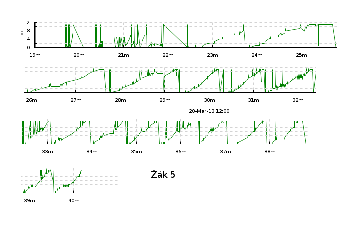
\includegraphics[width=1\textwidth]{Location5-cut}

Četl 17 řádků. Na grafu je 17 vrcholů, což odpovídá.

Dlouho jsem uvažoval, jak měřit rychlost čtení na FCHADu.  Sice mám hezké grafy, ale to neznamená, že mohu přesně měřit rychlost čtení.  Nezpracovaná data pro první tří písmena druhého řádku jsou (trojtečky značí, kde došlo ke změně dotýkaných senzorů, ale zobrazené písmeno se nezměnilo):
\begin{verbatim}
2013-03-20@12:23:44.436 Dolu  1 0 0 0 0 0 0 0 0 0 0 0 0 'k'
...
2013-03-20@12:23:49.634 Dolu  1 1 1 0 0 0 0 0 0 0 0 0 0 'k'
2013-03-20@12:23:49.964 Nahoru  0 1 1 0 0 0 0 0 0 0 0 0 1 'ý'
2013-03-20@12:23:50.129 Nahoru  0 1 0 0 0 0 0 0 0 0 0 0 1 'ý'
2013-03-20@12:23:50.212 Dolu  0 1 1 0 0 0 0 0 0 0 0 0 1 'ý'
2013-03-20@12:23:50.748 Dolu  1 1 1 0 0 0 0 0 0 0 0 0 0 'k'
2013-03-20@12:23:58.084 Nahoru 0 1 1 0 0 0 0 0 0 0 0 0 1 'ý'
2013-03-20@12:24:03.483 Dolu  0 1 1 1 0 0 0 0 0 0 0 0 1 'ý'
2013-03-20@12:24:03.525 Nahoru  0 0 1 1 0 0 0 0 0 0 0 0 2 ' '
...
2013-03-20@12:24:11.233 Dolu  0 0 1 1 1 0 0 0 0 0 0 0 2 ' '

\end{verbatim}

Nuly a jedničky značí, zda byl senzor aktivní. Například řádek
\begin{verbatim}
2013-03-20@12:24:11.233 Dolu  0 0 1 1 1 0 0 0 0 0 0 0 2 ' '
\end{verbatim}

znamená, že v 12:24:11.233 došlo k dotyku na třech senzorech a že se zobrazovala mezera.  Když se podíváte na čas 12:23:50.212, začíná se zobrazovat `ý', ale v 12:23:50.748 se vrací `k'.  Není z toho jasné, kdy čtení jednoho písmene končí a kdy čtení dalšího začíná.  Všechna shromážděná data jsou takto nejasná.  Proto jsem si vybral způsob analýzy očima za pomoci kružítka.

Pátý žák se během našeho setkání značně zrychlil.

Prvních pět řádků se zrychloval každým řádkem, ale mezi pátým řádkem a šestým řádkem není rozdíl v rychlosti. Sedmý řádek četl zase pomaleji, ale osmý řádek byl jeho nejrychlejší řádek vůbec. Devátý řádek zase četl stejně rychle jako pátý.  Na desátém řádku zpomalil.  Zbytek času zrychloval nebo zpomaloval bez rozpoznatelné tendence.

Nelze přesně měřit čas čtení na FCHADu, ale mohl jsem měřit čas od chvíle, kdy žák poprvé umístil ruku na selektor, do chvíle, kdy ji naposledy stáhl. Žák 5 četl na FCHADu jenom 17:02 minut a za tu dobu přečetl 196 znaků.  To je přibližně 0.2 znaků za sekundu. Když to srovnáme s jeho rychlostí čtení tištěného textu (11.37 CPS), vidíme, že na FCHADu během našeho setkání četl až 60krát pomaleji.

\subsection{Žák 6}
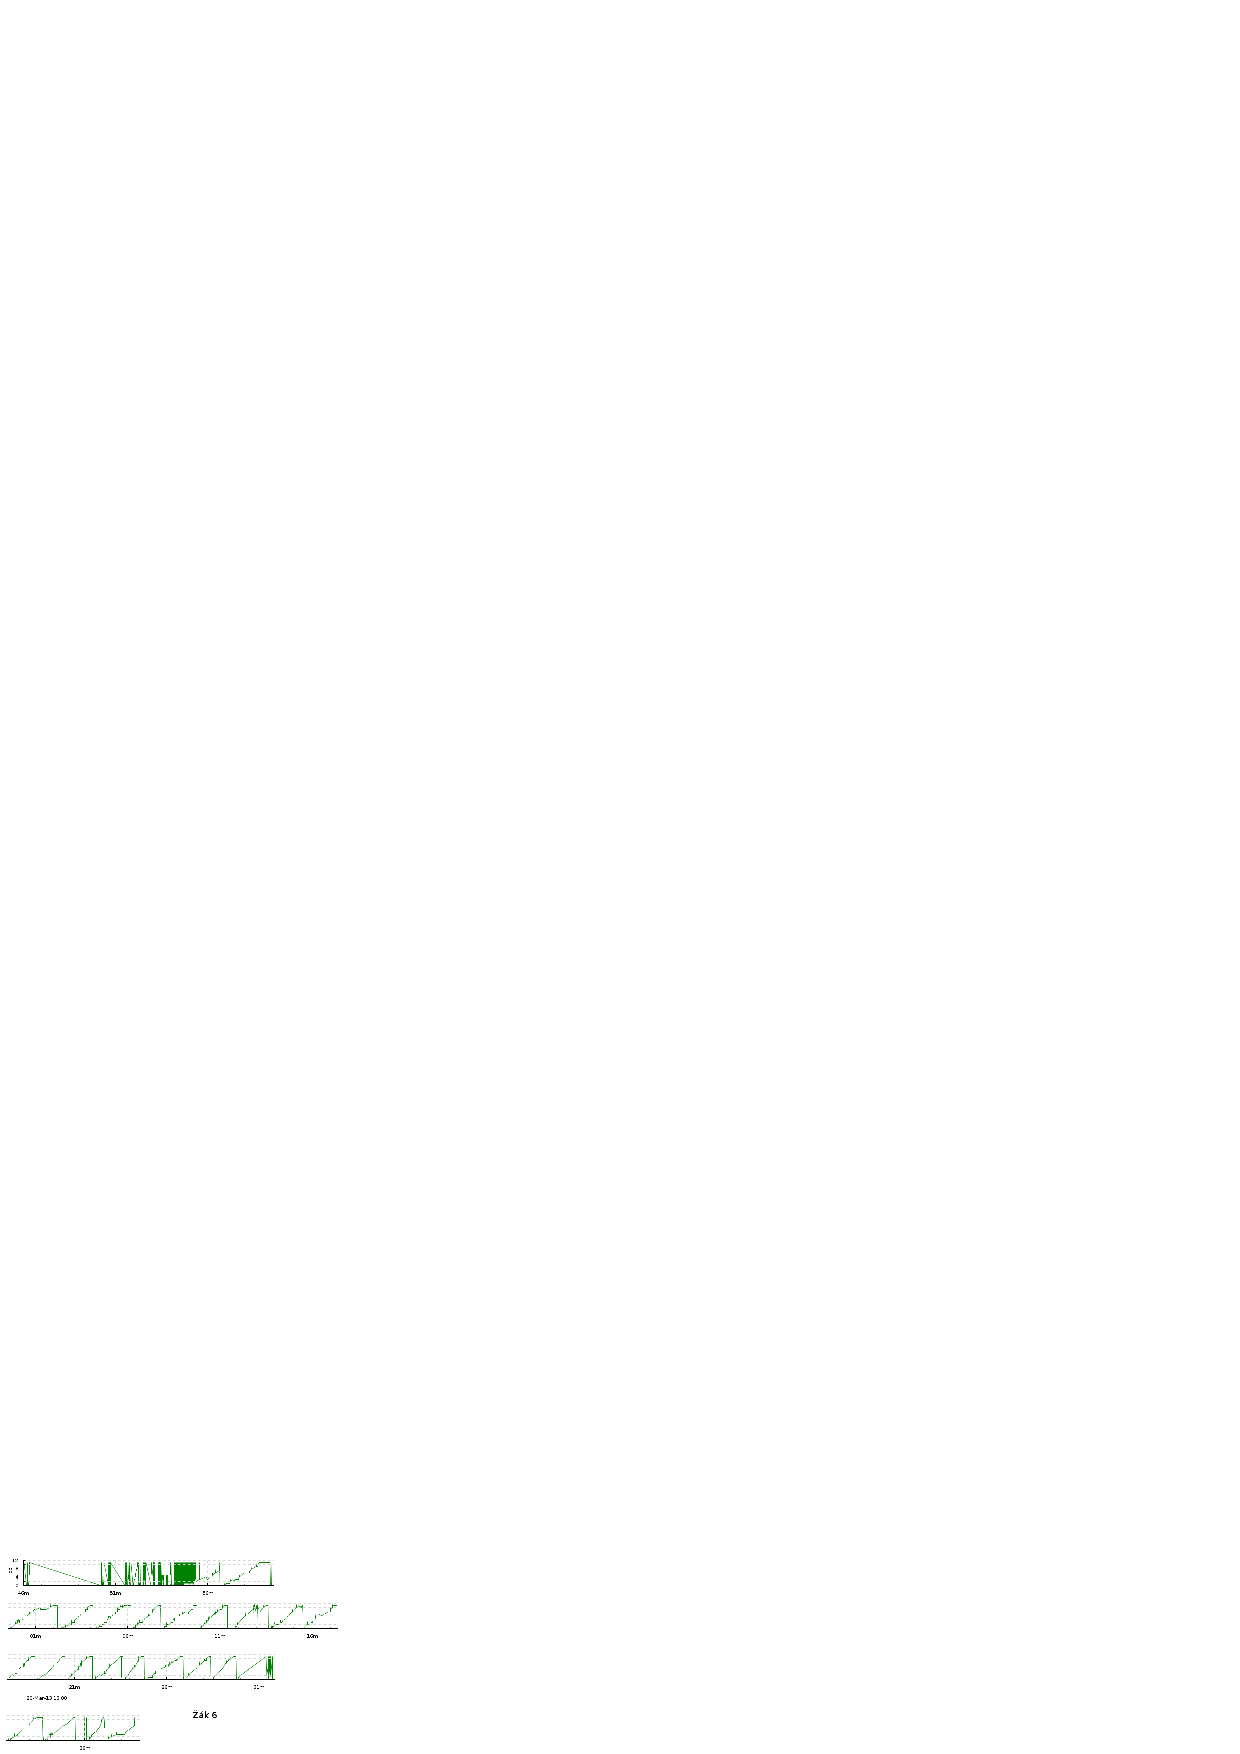
\includegraphics[width=1\textwidth]{Location6-cut}

Četla 22 řádků, přičemž z posledního jenom prvních 7 znaků.  Na grafu je 24 vrcholů: Vrchol s rovnou čárou kolem 31m není čtení (pouze přejetí prstem po senzorech) a předposlední řádek četla dvakrát.

Žákyně 6 se také zrychlila, ale ne tak pravidelně jako žák 5.

Druhý a třetí řádek četla stejně rychle.  Čtvrtý řádek četla rychleji, ale u pátého řádku trochu zpomalila. Dále nebyla tendence rozeznatelná.  Mezi řádky 12 a 16 se pomalu zrychlovala, ale na řádku 17 opět značně zpomalila.  Dále nelze rozeznat tendenci.  Předposlední řádek, kdy měla číst slova a ne písmena, a který četla podruhé, četla značně rychleji.

Žákyně 6 přečetla na FCHADu 249 znaků během 44:42 minut.  To je kolem 0.09 znaků za sekundu. Když to srovnáme s její rychlostí čtení tištěného textu (6.7 CPS), vidíme, že na FCHADu četla během našeho setkání až 72krát pomaleji.


\subsection{Žák 7}
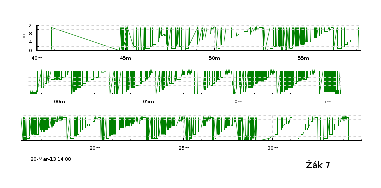
\includegraphics[width=1\textwidth]{Location7-cut}

Četl 19 řádků. Desátý řádek četl dvakrát, proto je na grafu dvacet vrcholů.

První čtyři řádky četl stejnou rychlostí. Během čtení pátého řádku odstranil prst ze selektoru, proto je vrchol na grafu rozdělený. Šestý řádek četl rychleji než ty první, ale pak se jeho rychlost nezměnila až do třináctého řádku, kdy zase zrychlil.  Čtrnáctý řádek je pomalý, ale zbytek doby zrychloval.


Žák 7 přečetl na FCHADu 215 znaků během 48:48 minut.  To je kolem 0.07 znaků za sekundu. Když to srovnáme s jeho rychlostí čtení tištěného textu (8.24 CPS), vidíme, že na FCHADu četl během našeho setkání až 112krát pomaleji.

\subsection{Žák 9}
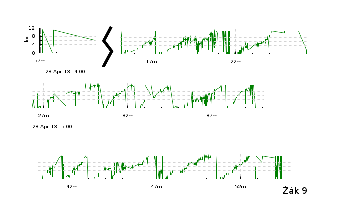
\includegraphics[width=1\textwidth]{Location9-cut}

Četl 13 řádků, na grafu je 13 vrcholů.

První čtyři řádky četl stejnou rychlostí, pátý řádek byl rychlejší a šestý stejně rychlý jako pátý. Sedmý je pomalý, ale na osmém až desátém zrychloval.  Velké zpomalení je vidět u jedenáctého řádku, snad proto, že jsou tam čísla. A poslední dva řádky jsou pomalé, protože používal selektor samostatně.

Žák 9 přečetl na FCHADu 148 znaků během 39:12 minut.  To je kolem 0.06 znaků za sekundu. Když to srovnáme s jeho rychlostí čtení tištěného textu (5 CPS), vidíme, že na FCHADu četl během našeho setkání až 79krát pomaleji.

Je jasné, že pokud jde o rychlost, je co zlepšovat.

\subsection{Analýza chyb}

Zde uvádím shromážděné chyby účastníků hlavní studie.  Opět vynechávám výsledky účastníka 8.

\begin{tabular}{|c|c|}
\hline
Symbol&Význam\\
\hline
NČ&Nečetl samostatně\\
\hline
??&Chyba, ale na nahrávce nebylo poznat jaká\\
\hline
>>&Přeskočil písmeno\\
\hline
*&Na nahrávce není poznat, zda udělal chybu\\
\hline
ZVP&Znak pro velká písmena\\
\hline
--&Četl s pomocí\\
\hline
\end{tabular}


%\paragraph{První Řádek}
\begin{tabular}{|c|c|c|c|c|c|c|c|c|c|c|c|c|}
\hline
Žák&B&r&a&i&l&l&s&&&&&\\
&\braillebox{1278}&\braillebox{1235}&\braillebox{1}&\braillebox{24}&\braillebox{123}&\braillebox{123}&\braillebox{234}&\braillebox{}&\braillebox{2358}&\braillebox{123}&\braillebox{}&\braillebox{}\\
\hline
5&&NČ&NČ&s&&&&>>&>>&>>&>>&>>\\
&&&&\braillebox{234}&&&&&&&&\\
\hline
6&v&&&&??&&&>>&>>&>>&>>&>>\\
&\braillebox{1236}&&&&&&&&&&&\\
\hline
7&ě&h&&,&&>>&&>>&>>&>>&>>&>>\\
&\braillebox{126}&\braillebox{125}&&\braillebox{2}&&&&&&&&\\
\hline
9&NČ&--&&&&&p&>>&>>&>>&>>&>>\\
&&&&&&&\braillebox{1234}&&&&&\\
\hline
\end{tabular}

%\paragraph{Druhý Řádek}
\begin{tabular}{|c|c|c|c|c|c|c|c|c|c|c|c|c|}
\hline
Žák&k&ý& &ř&á&d&e&k&,& &k&t\\
&\braillebox{1378}&\braillebox{12346}&\braillebox{}&\braillebox{2456}&\braillebox{16}&\braillebox{145}&\braillebox{15}&\braillebox{13}&\braillebox{2}&\braillebox{}&\braillebox{13}&\braillebox{2345}\\
\hline
5&&&&&&&&&NČ&&&\\
\hline
6&a&?p?&&?t?&&&??&&NČ&&&j\\
&\braillebox{1}&\braillebox{1234}&&\braillebox{2345}&&&&&&&&\braillebox{245}\\
\hline
7&&&&&&&&&&&&\\
\hline
9&&&&&&&&&&&a&\\
&&&&&&&&&&&\braillebox{1}&\\
\hline
\end{tabular}

%\paragraph{Třetí Řádek}
\begin{tabular}{|c|c|c|c|c|c|c|c|c|c|c|c|c|}
\hline
Žák&e&r&ý& &t&e&ď& &p&o&u&ž\\
&\braillebox{1578}&\braillebox{1235}&\braillebox{12346}&\braillebox{}&\braillebox{2345}&\braillebox{15}&\braillebox{1456}&\braillebox{}&\braillebox{1234}&\braillebox{135}&\braillebox{136}&\braillebox{2346}\\
\hline
5&&&&&&??&&&&&&\\
\hline
6&&&&&&&&&&r&&\\
&&&&&&&&&&\braillebox{1235}&&\\
\hline
7&&&&&&o&&&&k&&\\
&&&&&&\braillebox{135}&&&&\braillebox{13}&&\\
\hline
9&&&&&&&&&&&&z\\
&&&&&&&&&&&&\braillebox{1356}\\
\hline
\end{tabular}

%\paragraph{Čtvrtý Řádek}
\begin{tabular}{|c|c|c|c|c|c|c|c|c|c|c|c|c|}
\hline
Žák&í&v&á&t&e&,& &n&e&n&í& \\
&\braillebox{3478}&\braillebox{1236}&\braillebox{16}&\braillebox{2345}&\braillebox{15}&\braillebox{2}&\braillebox{}&\braillebox{1345}&\braillebox{15}&\braillebox{1345}&\braillebox{34}&\braillebox{}\\
\hline
5&&&&j&&&&d&&&&\\
&&&&\braillebox{245}&&&&\braillebox{145}&&&&\\
\hline
6&&l&&&&&&&&&&\\
&&\braillebox{123}&&&&&&&&&&\\
\hline
7&&&u&&o&&&d&&&&\\
&&&\braillebox{136}&&\braillebox{135}&&&\braillebox{145}&&&&\\
\hline
9&á&&&&i&&&ž(NČ)&>>&>>&t,á&\\
&\braillebox{16}&&&&\braillebox{24}&&&\braillebox{2346}&&&\braillebox{2345},\braillebox{16}&\\
\hline
\end{tabular}

%\paragraph{Pátý Řádek}
\begin{tabular}{|c|c|c|c|c|c|c|c|c|c|c|c|c|}
\hline
Žák&p&r&v&n&í& &ř&á&d&e&k&,\\
&\braillebox{123478}&\braillebox{1235}&\braillebox{1236}&\braillebox{1345}&\braillebox{34}&\braillebox{}&\braillebox{1235}&\braillebox{16}&\braillebox{145}&\braillebox{15}&\braillebox{13}&\braillebox{2}\\
\hline
5&&&&&&&&&&&&\\
\hline
6&&&&&&&&&&&a&NČ\\
&&&&&&&&&&&\braillebox{1}&\\
\hline
7&&&&&&*&*&*&*&*&*&*\\
\hline
9&&&&&&&&í&&&a&\\
&&&&&&&&\braillebox{34}&&&\braillebox{1}&\\
\hline
\end{tabular}

%\paragraph{Šestý Řádek}
\begin{tabular}{|c|c|c|c|c|c|c|c|c|c|c|c|c|}
\hline
Žák& &k&t&e&r&ý& &z&o&b&r&a\\
&\braillebox{78}&\braillebox{13}&\braillebox{2345}&\braillebox{15}&\braillebox{1235}&\braillebox{12346}&\braillebox{}&\braillebox{1356}&\braillebox{135}&\braillebox{12}&\braillebox{1235}&\braillebox{1}\\
\hline
5&&&&&&&&&&&&\\
\hline
6&&&&&&&&&&&&\\
\hline
7&&&&&&&&ř&&&&\\
&&&&&&&&\braillebox{2456}&&&&\\
\hline
9&&&&&&&&n&&&h&\\
&&&&&&&&\braillebox{1345}&&&\braillebox{125}&\\
\hline
\end{tabular}

%\paragraph{Řádek 7}
\begin{tabular}{|c|c|c|c|c|c|c|c|c|c|c|c|c|}
\hline
Žák&z&u&j&e& &j&e&n&o&m& &j\\
&\braillebox{135678}&\braillebox{136}&\braillebox{245}&\braillebox{15}&\braillebox{}&\braillebox{245}&\braillebox{15}&\braillebox{1345}&\braillebox{135}&\braillebox{134}&\braillebox{}&\braillebox{245}\\
\hline
5&&&&&&&&&&&&\\
\hline
6&&&&&&&&d&&&&\\
&&&&&&&&\braillebox{145}&&&&\\
\hline
7&&&&&&&&&&&&\\
\hline
9&n&a&h&&&h&&d&&k&&,\\
&\braillebox{1345}&\braillebox{1}&\braillebox{125}&&&\braillebox{125}&&\braillebox{145}&&\braillebox{13}&&\braillebox{2}\\
\hline
\end{tabular}

%\paragraph{Řádek 8}
\begin{tabular}{|c|c|c|c|c|c|c|c|c|c|c|c|c|}
\hline
Žák&e&d&n&o& &p&í&s&m&e&n&o\\
&\braillebox{1578}&\braillebox{145}&\braillebox{1345}&\braillebox{135}&\braillebox{}&\braillebox{1234}&\braillebox{34}&\braillebox{234}&\braillebox{134}&\braillebox{15}&\braillebox{1345}&\braillebox{135}\\
\hline
5&&&&&&&&&&&&\\
\hline
6&&&&&&&&&&&&\\
\hline
7&&&&&&&&??&&&&a\\
&&&&&&&&&&&&\braillebox{1}\\
\hline
9&&&&&&&á&&c&o&&e\\
&&&&&&&\braillebox{16}&&\braillebox{14}&\braillebox{135}&&\braillebox{15}\\
\hline
\end{tabular}

%\paragraph{Řádek 9}
\begin{tabular}{|c|c|c|c|c|c|c|c|c|c|c|c|c|}
\hline
Žák&.& & &P&r&v&n&í& &b&y&l\\
&\braillebox{378}&\braillebox{}&\braillebox{}&\braillebox{12347}&\braillebox{1235}&\braillebox{1236}&\braillebox{1345}&\braillebox{34}&\braillebox{}&\braillebox{12}&\braillebox{13456}&\braillebox{123}\\
\hline
5&&&&&&&&&&&&\\
\hline
6&NČ&&&&&&&&&&&\\
\hline
7&&&&&&&&&&&&\\
\hline
9&(,ZVP&&&&&&&&&&&\\
&\braillebox{236},\braillebox{6}&&&&&&&&&&&\\
\hline
\end{tabular}

%\paragraph{Řádek 10}
\begin{tabular}{|c|c|c|c|c|c|c|c|c|c|c|c|c|}
\hline
Žák& &v&y&n&a&l&e&z&e&n& &v\\
&\braillebox{78}&\braillebox{1236}&\braillebox{13456}&\braillebox{1345}&\braillebox{1}&\braillebox{123}&\braillebox{15}&\braillebox{1356}&\braillebox{15}&\braillebox{1345}&\braillebox{}&\braillebox{1236}\\
\hline
5&&&&&&&&&&&&\\
\hline
6&&&?ď ?&&&&&&&&&\\
&&&\braillebox{1456}&&&&&&&&&\\
\hline
7&&??&&&&&o&&&&&\\
&&&&&&&\braillebox{135}&&&&&\\
\hline
9&&&&&&b&&&&&&\\
&&&&&&\braillebox{12}&&&&&&\\
\hline
\end{tabular}

%\paragraph{Řádek 11}
\begin{tabular}{|c|c|c|c|c|c|c|c|c|c|c|c|c|}
\hline
Žák& &r&o&c&e& &1&9&1&3& &v\\
&\braillebox{78}&\braillebox{1235}&\braillebox{135}&\braillebox{14}&\braillebox{15}&\braillebox{}&\braillebox{18}&\braillebox{248}&\braillebox{18}&\braillebox{148}&\braillebox{}&\braillebox{1236}\\
\hline
5&&&&&&&&&&&&\\
\hline
6&&&&&&&a&i&&&&\\
&&&&&&&\braillebox{1}&\braillebox{24}&&&&\\
\hline
7&&&&n&&&a&i&&&&l,r\\
&&&&\braillebox{1345}&&&\braillebox{1}&\braillebox{24}&&&&\braillebox{123},\braillebox{1235}\\
\hline
9&&ř&e,a&&&&a&i&&&&\\
&&\braillebox{2456}&\braillebox{15},\braillebox{1}&&&&\braillebox{1}&\braillebox{24}&&&&\\
\hline
\end{tabular}

%\paragraph{Řádek 12}
\begin{tabular}{|c|c|c|c|c|c|c|c|c|c|c|c|c|}
\hline
Žák& &A&n&g&l&i&i&.& & &J&m\\
&\braillebox{78}&\braillebox{17}&\braillebox{1345}&\braillebox{1245}&\braillebox{123}&\braillebox{24}&\braillebox{24}&\braillebox{3}&\braillebox{}&\braillebox{}&\braillebox{2457}&\braillebox{134}\\
\hline
5&&&d&&&&&mezera&&&&\\
&&&\braillebox{145}&&&&&\braillebox{}&&&&\\
\hline
6&&&&&&&9&&&&--&\\
&&&&&&&\braillebox{248}&&&&&\\
\hline
7&&&&&&e&&&&&&\\
&&&&&&\braillebox{15}&&&&&&\\
\hline
9&&&d&x&b&&&&&&,&c\\
&&&\braillebox{145}&\braillebox{1346}&\braillebox{12}&&&&&&\braillebox{2}&\braillebox{14}\\
\hline
\end{tabular}

%\paragraph{Řádek 13}
\begin{tabular}{|c|c|c|c|c|c|c|c|c|c|c|c|c|}
\hline
Žák&e&n&o&v&a&l& &s&e& &O&p\\
&\braillebox{1578}&\braillebox{1345}&\braillebox{135}&\braillebox{1236}&\braillebox{1}&\braillebox{123}&\braillebox{}&\braillebox{234}&\braillebox{15}&\braillebox{}&\braillebox{1357}&\braillebox{1234}\\
\hline
5&&&&&&&&&&&n&\\
&&&&&&&&&&&\braillebox{1345}&\\
\hline
6&*&*&r&&&&&&&&&\\
&&&\braillebox{1235}&&&&&&&&&\\
\hline
7&&&&l&&&&&&&&\\
&&&&\braillebox{123}&&&&&&&&\\
\hline
9&&&e&&&&&&&&k&l\\
&&&\braillebox{15}&&&&&&&&\braillebox{13}&\braillebox{123}\\
\hline
\end{tabular}

%\paragraph{Řádek 14}
\begin{tabular}{|c|c|c|c|c|c|c|c|c|c|c|c|c|}
\hline
Žák&t&o&f&o&n& &a& &p&ř&e&v\\
&\braillebox{234578}&\braillebox{135}&\braillebox{124}&\braillebox{135}&\braillebox{1345}&\braillebox{}&\braillebox{1}&\braillebox{}&\braillebox{1234}&\braillebox{2456}&\braillebox{15}&\braillebox{1236}\\
\hline
5&&&&&&&&&&&&\\
\hline
6&j&&&&&&&&n&&&\\
&\braillebox{245}&&&&&&&&\braillebox{1345}&&&\\
\hline
7&&&&&&&&&&&&\\
\hline
\end{tabular}

%\paragraph{Řádek 15}
\begin{tabular}{|c|c|c|c|c|c|c|c|c|c|c|c|c|}
\hline
Žák&á&d&ě&l& &s&v&ě&t&l&o& \\
&\braillebox{1678}&\braillebox{145}&\braillebox{126}&\braillebox{123}&\braillebox{}&\braillebox{234}&\braillebox{1236}&\braillebox{126}&\braillebox{2345}&\braillebox{123}&\braillebox{135}&\braillebox{}\\
\hline
5&&&&&&&&&&&&\\
\hline
6&&&v&&&i&&&j&&&\\
&&&\braillebox{1236}&&&\braillebox{15}&&&\braillebox{245}&&&\\
\hline
7&&&&&&&&&&&&\\
\hline
\end{tabular}

%\paragraph{Řádek 16}
\begin{tabular}{|c|c|c|c|c|c|c|c|c|c|c|c|c|}
\hline
Žák&n&a& &z&v&u&k&.& & &K&d\\
&\braillebox{134578}&\braillebox{1}&\braillebox{}&\braillebox{1356}&\braillebox{1236}&\braillebox{136}&\braillebox{13}&\braillebox{3}&\braillebox{}&\braillebox{}&\braillebox{137}&\braillebox{145}\\
\hline
5&&&&e&&&&&&&&\\
&&&&\braillebox{15}&&&&&&&&\\
\hline
6&&&&&&&&&&&&\\
\hline
7&&&&&&&&&&&&\\
\hline
\end{tabular}

%\paragraph{Řádek 17}
\begin{tabular}{|c|c|c|c|c|c|c|c|c|c|c|c|c|}
\hline
Žák&y&ž& &č&t&e&n&á&ř& &p&o\\
&\braillebox{1345678}&\braillebox{2346}&\braillebox{}&\braillebox{146}&\braillebox{2345}&\braillebox{15}&\braillebox{1345}&\braillebox{16}&\braillebox{2456}&\braillebox{}&\braillebox{1234}&\braillebox{135}\\
\hline
5&&&&&&&&&&&&\\
\hline
6&&&&&j&&k&&&&&\\
&&&&&\braillebox{245}&&\braillebox{13}&&&&&\\
\hline
7&ď&&&??&&&&&&&&\\
&\braillebox{1456}&&&&&&&&&&&\\
\hline
\end{tabular}

%\paragraph{Řádek 18}
\begin{tabular}{|c|c|c|c|c|c|c|c|c|c|c|c|c|}
\hline
Žák&h&y&b&o&v&a&l& &s&p&e&c\\
&\braillebox{12578}&\braillebox{13456}&\braillebox{12}&\braillebox{135}&\braillebox{1236}&\braillebox{1}&\braillebox{123}&\braillebox{}&\braillebox{234}&\braillebox{1234}&\braillebox{15}&\braillebox{14}\\
\hline
6&&&&&&&&&&&&\\
\hline
7&??&d&&&&&&&&&&\\
&&\braillebox{145}&&&&&&&&&&\\
\hline
\end{tabular}

%\paragraph{Řádek 19}
\begin{tabular}{|c|c|c|c|c|c|c|c|c|c|c|c|c|}
\hline
Žák&i&á&l&n&í&m& &p&e&r&e&m\\
&\braillebox{2478}&\braillebox{16}&\braillebox{123}&\braillebox{1345}&\braillebox{34}&\braillebox{134}&\braillebox{}&\braillebox{1234}&\braillebox{15}&\braillebox{1235}&\braillebox{15}&\braillebox{134}\\
\hline
6&&&&&&&&&&&&\\
\hline
7&s&e&&&&&&&o&&&p\\
&\braillebox{234}&\braillebox{15}&&&&&&&\braillebox{135}&&&\braillebox{1234}\\
\hline
\end{tabular}

%\paragraph{Řádek 20}
\begin{tabular}{|c|c|c|c|c|c|c|c|c|c|c|c|c|}
\hline
Žák& &n&a&d& &p&í&s&m&e&n&e\\
&\braillebox{78}&\braillebox{1345}&\braillebox{1}&\braillebox{145}&\braillebox{}&\braillebox{1234}&\braillebox{34}&\braillebox{234}&\braillebox{134}&\braillebox{15}&\braillebox{1345}&\braillebox{15}\\
\hline
6&&&&&&&&&&&&\\
\hline
\end{tabular}

%\paragraph{Řádek 21}
\begin{tabular}{|c|c|c|c|c|c|c|c|c|c|c|c|c|}
\hline
Žák&m&,& &p&ř&í&s&t&r&o&j& \\
&\braillebox{13478}&\braillebox{2}&\braillebox{}&\braillebox{1234}&\braillebox{2456}&\braillebox{34}&\braillebox{234}&\braillebox{2345}&\braillebox{1235}&\braillebox{135}&\braillebox{245}&\braillebox{}\\
\hline
6&&&&&&&&&&&&\\
\hline
\end{tabular}

%\paragraph{Řádek 22}
\begin{tabular}{|c|c|c|c|c|c|c|c|c|c|c|c|c|}
\hline
Žák&b&z&u&č&e&l&.& & &T&o& \\
&\braillebox{1278}&\braillebox{1356}&\braillebox{136}&\braillebox{146}&\braillebox{15}&\braillebox{123}&\braillebox{3}&\braillebox{}&\braillebox{}&\braillebox{23457}&\braillebox{135}&\braillebox{}\\
\hline
6&&&&&&&&>>&>>&>>&>>&>>\\
\hline
\end{tabular}
\clearpage
\begin{figure}
\subsection{Druhy chyb}
\begin{subfigure}{.5\textwidth}
\centering
Zrcadlení - převážně u žáka 9

\begin{tabular}{|c|c|c|}
\hline
Počet&Správné písmeno&Chybné písmeno\\
\hline
1&ž\braillebox{2346}&z\braillebox{1356}\\
\hline
1&í\braillebox{3478}&á\braillebox{16}\\
\hline
2&í\braillebox{34}&á\braillebox{16}\\
\hline
1&e\braillebox{15}&i\braillebox{24}\\
\hline
1&i\braillebox{24}&e\braillebox{15}\\
\hline
1&n\braillebox{1345}&ž\braillebox{2346}\\
\hline
1&z\braillebox{1356}&n\braillebox{1345}\\
\hline
1&z\braillebox{135678}&n\braillebox{1345}\\
\hline
2&j\braillebox{245}&h\braillebox{125}\\
\hline
1&.\braillebox{378}&ZVP\braillebox{6}\\
\hline
1&r\braillebox{1235}&ř\braillebox{2456}\\
\hline
14\\
\hline
\end{tabular}
\end{subfigure}
\begin{subfigure}{.5\textwidth}
\centering
Nečetl dolní bod

\begin{tabular}{|c|c|c|}
\hline
Počet&Správné\newline písmeno&Chybné písmeno\\
\hline
2&r\braillebox{1235}&h\braillebox{125}\\
\hline
1&k\braillebox{1378}&a\braillebox{1}\\
\hline
3&k\braillebox{13}&a\braillebox{1}\\
\hline
1&ý\braillebox{12346}&p\braillebox{1234}\\
\hline
4&t\braillebox{2345}&j\braillebox{245}\\
\hline
1&t\braillebox{234578}&j\braillebox{245}\\
\hline
6&n\braillebox{1345}&d\braillebox{145}\\
\hline
1&u\braillebox{136}&a\braillebox{1}\\
\hline
2&m\braillebox{134}&c\braillebox{14}\\
\hline
3&o\braillebox{135}&e\braillebox{15}\\
\hline
2&l\braillebox{123}&b\braillebox{12}\\
\hline
1&y\braillebox{13456}&ď\braillebox{1456}\\
\hline
1&y\braillebox{1345678}&ď\braillebox{1456}\\
\hline
1&y\braillebox{1345678}&d\braillebox{145}\\
\hline
1&z\braillebox{1356}&e\braillebox{15}\\
\hline
30\\
\hline
\end{tabular}
\end{subfigure}

\begin{subfigure}{1\textwidth}
\centering
Body sedm a osm je mátly

\begin{tabular}{|c|c|c|}
\hline
Počet&Správné písmeno&Chybné písmeno\\
\hline
1&B\braillebox{1278}&v\braillebox{1236}\\
\hline
1&B\braillebox{1278}&ě\braillebox{126}\\
\hline
3&1\braillebox{18}&a\braillebox{1}\\
\hline
1&i\braillebox{24}&9\braillebox{248}\\
\hline
3&9\braillebox{248}&i\braillebox{24}\\
\hline
9\\
\hline
\end{tabular}
\end{subfigure}
\end{figure}
\begin{figure}
\begin{subfigure}{.5\textwidth}
\centering
Nečetli pravý sloupec bodů

\begin{tabular}{|c|c|c|}
\hline
Počet&Správné písmeno&Chybné písmeno\\
\hline
1&i\braillebox{24}&,\braillebox{2}\\
\hline
1&o\braillebox{135}&k\braillebox{13}\\
\hline
1&v\braillebox{1236}&l\braillebox{123}\\
\hline
1&m\braillebox{134}&k\braillebox{13}\\
\hline
2&j\braillebox{245}&,\braillebox{2}\\
\hline
2&v\braillebox{1236}&l\braillebox{123}\\
\hline
1&O\braillebox{1357}&k\braillebox{13}\\
\hline
1&p\braillebox{1234}&l\braillebox{123}\\
\hline
1&n\braillebox{1345}&k\braillebox{13}\\
\hline
11\\
\hline
\end{tabular}
\end{subfigure}
\begin{subfigure}{.5\textwidth}
\centering
Přidali nějaký bod

\begin{tabular}{|c|c|c|}
\hline
Počet&Správné písmeno&Chybné písmeno\\
\hline
2&i\braillebox{24}&s\braillebox{234}\\
\hline
1&s\braillebox{23478}&i\braillebox{15}\\
\hline
1&s\braillebox{234}&p\braillebox{1234}\\
\hline
5&e\braillebox{15}&o\braillebox{135}\\
\hline
2&o\braillebox{135}&r\braillebox{1235}\\
\hline
1&á\braillebox{16}&u\braillebox{136}\\
\hline
1&ě\braillebox{126}&v\braillebox{1236}\\
\hline
1&m\braillebox{134}&p\braillebox{1234}\\
\hline
14\\
\hline
\end{tabular}
\end{subfigure}
\begin{subfigure}{1\textwidth}
\centering
Nemám vysvětlení / Jiné

\begin{tabular}{|c|c|c|}
\hline
Počet&Správné písmeno&Chybné písmeno\\
\hline
1&ř\braillebox{2456}&t\braillebox{2345}\\
\hline
1&í\braillebox{34}&t\braillebox{2345}\\
\hline
1&z\braillebox{1345}&ř\braillebox{2456}\\
\hline
1&.\braillebox{378}&(\braillebox{236}\\
\hline
1&c\braillebox{14}&n\braillebox{1345}\\
\hline
1&v\braillebox{1236}&r\braillebox{1235}\\
\hline
1&g\braillebox{1245}&x\braillebox{1346}\\
\hline
1&O\braillebox{1357}&n\braillebox{1345}\\
\hline
1&p\braillebox{1234}&n\braillebox{1345}\\
\hline
1&á\braillebox{16}&e\braillebox{15}\\
\hline
10\\
\hline
\end{tabular}
\end{subfigure}
\end{figure}

\clearpage
\subsection{Počty chyb}
Žák 5 udělal 8 chyb na 196 přečtených znaků: jedna chyba na 24.5 znaků.

Žákyně 6 udělala 24 chyb na 249 přečtených znaků: jedna chyba na 10.375 znaků.

Žák 7 udělal 27 chyb na 215 přečtených znaků: jedna chyba na 7.963\_{} znaků

Žák 9 udělal 37 chyb na 148 přečtených znaků: jedna chyba na 4 znaky

Zde je tabulka počtů chyb na znak:

\begin{tabular}[hb]{|c|c|c|c|c|}
\hline
Řádek&Žák 5&Žák 6&Žák 7&Žák 9\\
\hline
1&$\frac{1}{5}$&$\frac{2}{7}$&$\frac{3}{6}$&$\frac{1}{6}$\\
\hline
2&$\frac{0}{12}$&$\frac{5}{11}$&$\frac{0}{12}$&$\frac{1}{12}$\\
\hline
3&$\frac{1}{12}$&$\frac{1}{12}$&$\frac{2}{12}$&$\frac{1}{12}$\\
\hline
4&$\frac{2}{12}$&$\frac{1}{12}$&$\frac{3}{12}$&$\frac{4}{10}$\\
\hline
5&$\frac{0}{12}$&$\frac{1}{11}$&$\frac{0}{5}$&$\frac{2}{12}$\\
\hline
6&$\frac{0}{12}$&$\frac{0}{12}$&$\frac{1}{12}$&$\frac{2}{12}$\\
\hline
7&$\frac{0}{12}$&$\frac{1}{12}$&$\frac{0}{12}$&$\frac{7}{12}$\\
\hline
8&$\frac{0}{12}$&$\frac{0}{12}$&$\frac{2}{12}$&$\frac{4}{12}$\\
\hline
9&$\frac{0}{12}$&$\frac{0}{11}$&$\frac{0}{12}$&$\frac{1}{12}$\\
\hline
10&$\frac{0}{12}$&$\frac{1}{12}$&$\frac{2}{12}$&$\frac{1}{12}$\\
\hline
11&$\frac{0}{12}$&$\frac{2}{12}$&$\frac{4}{12}$&$\frac{4}{12}$\\
\hline
12&$\frac{2}{12}$&$\frac{2}{12}$&$\frac{1}{12}$&$\frac{5}{12}$\\
\hline
13&$\frac{1}{12}$&$\frac{1}{10}$&$\frac{1}{12}$&$\frac{3}{12}$\\
\hline
14&$\frac{0}{12}$&$\frac{2}{12}$&$\frac{0}{12}$&\\
\hline
15&$\frac{0}{12}$&$\frac{3}{12}$&$\frac{0}{12}$&\\
\hline
16&$\frac{1}{12}$&$\frac{0}{12}$&$\frac{0}{12}$&\\
\hline
17&$\frac{0}{12}$&$\frac{2}{12}$&$\frac{2}{12}$&\\
\hline
18&&$\frac{0}{12}$&$\frac{2}{12}$&\\
\hline
19&&$\frac{0}{12}$&$\frac{4}{12}$&\\
\hline
20&&$\frac{0}{12}$&&\\
\hline
21&&$\frac{0}{12}$&&\\
\hline
22&&$\frac{0}{7}$&&\\
\hline
\end{tabular}

Žák 5 dělal chyby během prvních čtyř řádků.  Potom už chyby nedělal, kromě skupiny chyb v řádcích 12 a 13.

Žákyně 6 taky udělala většinu chyb na začátku čtení v řádcích jedna a dva.  Nebyla tak dokonalá jako žák 5, ale dělala méně chyb než jednu na řádek až po řádek 11, kde má taky skupinu řádků se zvýšenou chybovostí.

Žáci 7 a 9 nemají žádnou strukturu chybovosti.

\section{Analýza podle dříve uvedeného modelu}

\subsection{Swift}
Vrátíme-li se ke Swiftovu rozdělení druhů učení, vidíme, že moje studie obsahovala všechny tři druhy.

\textit{získání dovednosti, neboli naučit se něco dělat} :
Účastníci získali dovednost používat selektor.

\textit{získání znalostí, uvědomování souvislostí} :
Účastníci trénovali souvislost mezi malým Braillovým písmem, které již znají, a velkým, které se zobrazuje na zobrazovači FCHADu.

Účastníci také získali úplně novou znalost.  Například to, že Orca používá body sedm a osm naráz pro označení začátku řádku, je snad novinkou pro všechny účastníky.  Na tuto novou informaci si zvykli velmi rychle.  Stačilo jím říct jednou nebo dvakrát, co ty body znamenají, a už si to pamatovali po celé setkání.


\textit{získání sebekontroly a potlačení reflexů } :

Rozdělil bych Swiftovu kategorii získání sebekontroly a potlačení reflexů na dvě subkategorie:  potlačení reflexů a přeučení znalosti.

Účastníci si odvykli používat selektor jako piezoelektrický braillský řádek a tím pádem trénovali potlačení reflexů.  To jsem obzvlášť viděl u účastníků čtyři a pět.  Když se vrátili na začátek selektoru poté, co dočetli řádek, skoro vždy se vrátili příliš daleko, protože byli zvyklí na delší braillský řádek.  To je jev, který je docela podobný Swiftovu mrkání.

Sledoval jsem ještě další projev odvykání, který přímo do první skupiny nepatří, to když žák 9 četl `g'\braillebox{1245} jako `x'\braillebox{1346}. Je jasné, že je zvyklý na menší písmo, a když cítí, jak daleko od sebe jsou body na zobrazovači, tak myslí, že mezi nimi musí být nějaké neaktivní.  Nejedná se o reflex ani o návyk v chování, ale o návyk myšlení a paměti.  Návyk na menší písmo může vysvětlit mnoho chyb při čtení.  Žáci četli `k'\braillebox{13} jako `a'\braillebox{1} třikrát. Možná proto, že jsou zvyklí na o tolik menší `a', že ten třetí bod dole se jim ani nezdá být součástí toho samého písmena.

Kvůli časovému omezení jsme se tím moc nezabývali, ale někteří účastníci nepoložili ruku na zobrazovač rovně.  Do jisté míry může být jejich neochota vysvětlena tím, že jim není příjemné, jak jim kovové tyčky vráží do dlaně.  To je velice podobná reakce jako Swiftovo mrkání:  Nemáme rádi rychlé pohyby.

\subsection{Anderson}

\textit{kognitivní stadium}: Začátek kognitivního stadia představovalo přečtení návodu, ale probíhalo i později během čtení, například když jsem jim dával nové instrukce, když se dostali na konec řádku nebo na písmeno, které nepochopili.  Rozdělení fází není stoprocentní.

\textit{asociativní stadium}: Asociativní stadium trvalo po většinu času této studie.  Žáci zdokonalovali posun na selektoru a odstraňovali chyby při čtení na zobrazovači.

\textit{autonomní stadium}: Nenastalo. Účastníci autonomně nečetli.

\subsection{Vlastní model}

\textit{Předznalost}:
Jako pedagog jsem si všiml především nedostatku předznalosti.
Někteří žáci nedovedli říct, které písmeno tvoří body "jedna, dva, tři, pět"(`r'). Bylo mojí chybou jako pedagoga, že jsem nesprávně odhadl předznalost.  Předpokládal jsem, že budou znát číslování znaků. 

Dalším překvapením bylo, že snad jen jeden žák z hlavní studie už znal funkci bodů sedm a osm pro značení velkých písmen a číslic.  Myslel jsem, že i když tato funkce není standardizována, žáci hned pochopí, o co jde.

Dalším překvapením bylo, že snad žádný žák nepoznal čárku.

Účastníci, kteří nepoužívají braillský řádek, se museli učit daleko víc, ale zase to neznamenalo, že by dělali víc chyb. Individuální rozdíly jsou daleko výraznější než rozdíly mezi žáky, kteří řádky používají, a těmi, kteří je nepoužívají.  I kdyby čísla byla jednoznačná, neznamenalo by to automaticky, že měli horší výkon kvůli nedostatku předznalostí. Důvodem, proč předznalosti nemají, může být to, že jsou neschopní či neochotní se učit!

Při přípravě studie jsem význam předznalosti značně nadhodnotil.  Myslel jsem si, že já čtu na FCHADu pomalu, protože obecně neumím moc dobře číst rukama, zato lidé, kteří to umějí, budou schopní rychle číst i na FCHADu.  K mému překvapení jejich první pokusy nebyly o tolik úspěšnější než moje.

\em Chápání úkolu\em : Způsob výkladu byl hlavně čtení návodu.  Pomohl jsem jako pedagog tím, že jsem žáky při práci s nástrojem ústně a taktilně naváděl.  Ústní pomoc se od písemné neliší jenom tím, že probíhá přes zvukové medium, ale i tím, že žáci mohli klást otázky.

Protože žáci nebyli schopní \uv{číst} na FCHADu, rozdělil jsem úkol na konkrétnější zadání: \uv{číst první písmeno}.  Většina rozuměla, jak číst první písmeno, a ani jim netrvalo moc dlouho pochopit, jak postoupit na další písmeno za použití selektoru. Spojit oba podúkoly dohromady a skutečně číst jim však trvalo velmi dlouho.

\em Obecná schopnost\em a \em konkrétní schopnost\em :  Obecná schopnost, které jsem chtěl žáky naučit, byla číst na FCHADu.  Konkrétních schopností bylo několik:

Číst písmeno ze zobrazovače, což se dá rozdělit na ještě další konkrétní schopnosti, jako je čtení určitého písmene, například `e', nebo pochopení funkcí bodů sedm a osm.

Přesunout ruku na selektoru, aby se zobrazilo další písmeno.

Vrátit ruku na začátek selektoru, když začíná nový řádek.

Z těchto schopností byla snad jediná, kterou žáci dovedli rozvíjet na úrovni autonomní schopnosti, a to přesun ruky na selektoru.

\em Dosažená úroveň\em : V rámci této studie nemohu dojít k závěru o dosažené úrovni, protože žádný účastník tak daleko nedospěl.


\chapter{Závěr}
Čekal jsem, že to bude trvat déle rozumět stroj ale, že účastnici budou schopní rychlejší číst. Byl jsem překvapení z toho, že účastnici rozuměli základní fungování stroje skoro hned ale četli hodně pomalu. Některé účastnici skoro nezlepšili rychlost během setkání.

Začal jsem studie tím, že jsem chtěl vyzkoumat jak nevidomé lidí samy od sebe objevuji funkčnost nastroje. Moje účastnici byli až moc pasivní na to, a vždy čekali na můj příkaz. Asi se báli stroj, který vydá strašlivé cvaknutí když do ně dotykáte.

Měl jsem na mysl, že Andersonův kognitivní stadium bude trvat dlouho, že budou se strojem hrát. Třeba, kdybych čekal déle by hráli. Nikdy jsem je nedal přikázaní, že musejí čekat na moje potvrzení správné čtení aby pokračovali. Však, jsem je nikdy neříkal \uv{teď budeme drilovat čtení po jednotlivých písmenech}. Některé zvládly stroj dostatečně dobře, že samostatně četli par písmen ale do větší míru než ne spadli jsme do rigidní drilování, které jsem nikdy explicitně nepřikazoval. Během předběžní studium, stroj ještě byl dost vadní, že se rigidnost hodila ale u běžní studium už nebyl k tomu důvod. Asi \uv{čtení} má v sobě určíte míru rigiditu. Čteme z levá do práva od začátku ke konci není jiný způsob.

Účastnici byly snad jen tak zvykly čekat a poslouchat.

Vratíme-li k otázky uvedené v kapitole 1.5 Cíle Práce, už můžeme na některé z nich odpovědět.

\em Jakým způsobem lidé reagují na neznámým nastroj během prvních 45 minut používání? Jak oni přizpůsobují k novému nastroje? Jaké mají potom dojmy?\em  Moje účastnici velmi rychle pochopili fungování nastroje ale pomalu získali schopnost to pochopení používat.  Její důvěru v vlastní schopnost s naučit používat FCHAD byl přímo spojení tím jestli samy používali braillské řádky.

\em Jaká je role pedagoga v procesu podpory učení práce s novým nástrojem?\em Je snad jasný, že pro nevidomé lidí pedagog je nezbytný součásti proces učení neznámé nastroje.  Všechní účastníci potřebovali pomoc s orientaci s novým nástrojem a oprava chyb pří čtení.  Pedagogický intervence byl zvlášť nezbytný u žáka 9, který většina dobu čtení nezvládl vůbec číst samostatně.

Vice informace o teto studie nalezte v angličtině na webové strance: \footnote{\url{https://github.com/timthelion/fchad-study}}.  Veškeré otázky o projektu FCHAD pošlete Timothy Hobbs {\tt timothyhobbs@seznam.cz}.  Technické otázky o návrh braillských řádků pošlete na emailový seznam
\footnote{\url{ http://mielke.cc/brltty/contact.html#list}}.



\singlespacing
\bibliographystyle{csplainnat}
\bibliography{references}
~\\
~\\

\addcontentsline{toc}{chapter}{Literatura}

\clearpage{}

\appendix
\pagenumbering{Roman}
\thispagestyle{empty}  
\renewcommand{\appendixname}{Appendix}%%přílohy, číslování římskými


\chapter*{Appendix}
\addcontentsline{toc}{chapter}{Appendix}

\section*{Whatever}



\end{document}
